\section{Database}
Databasen anvendes i forbindelse med registrering af brugere. Derudover skal det være muligt for systemet at hente og gemme data i en database. Der blev opstillet følgende funktionelle krav til database:
 
\begin{itemize}
\item Brugere skal kunne oprettes i en database
\\
\textit{Dette er nødvendigt for, at brugere kan anvende app’en}
\item Systemet skal kunne gemme og hente data i en database
\\
\textit{Dette er nødvendigt for, at brugere kan tilgå brugerdata}
\end{itemize}

\noindent
For at teste om de opstillede krav til databasen er overholdt udføres testen, som fremgår af \autoref{tab:testDatabase}.

  \begin{longtable}{ | l | p{13cm} |} \hline
    \textbf{Test:} & Database \\ \hline
     \textbf{Formål:} & Formålet er at oprette brugere i databasen samt hente og sende data. Dette gøres ved at oprette en bruger i databasen. Efterfølgende vil en kategorisering foretages, og derefter tjekkes om denne er gemt i databasen. Til sidst skal brugeren gå til rediger adgangskode og tjekke om kategoriseringen er angivet og derved hentet fra databasen. \\ \hline
 	\textbf{Main flow:} & 1.~ Indtast SQL-forespørgsel \textit{INSERT INTO 'users' ('navn', 'medlemsid', 'db\_adgangskode', 'kategorisering') VALUES ('Jens Jensen', '11170301', 'adgangskode', 'F')} i databasen.
 	\begin{itemize}
	\item Bruger er oprettet i databasen 
	\end{itemize}
 2.~Åben app’en og log ind med medlemsID, \textit{11170301}, og adgangskode, \textit{adgangskode}. Udfør kategorisering og få en samlet CATscore under 10 ved at vælge værdierne \textit{0,1,2,1,0,1,0,1}, tryk videre efter hver angivet værdi. Herefter vælges antallet af indlæggelser til \textit{0 INDLÆGGELSER}. 
 \begin{itemize}
 \item Kategorisering A er gemt i databasen (\textbf{\textit{Figur 1 og 2}})
 \end{itemize}
3.~Tryk på \textit{REDIGER ADGANGSKODE} via hovedmenuen.
\begin{itemize}
\item MedlemsID og navn samt opdaterede kategorisering, A, vises under rediger adgangskode (\textbf{\textit{Figur 3}})
\end{itemize}
 \\  \hline
  \textbf{Resultat:} &
  \hspace{1.5mm}
 \raisebox{-\totalheight}{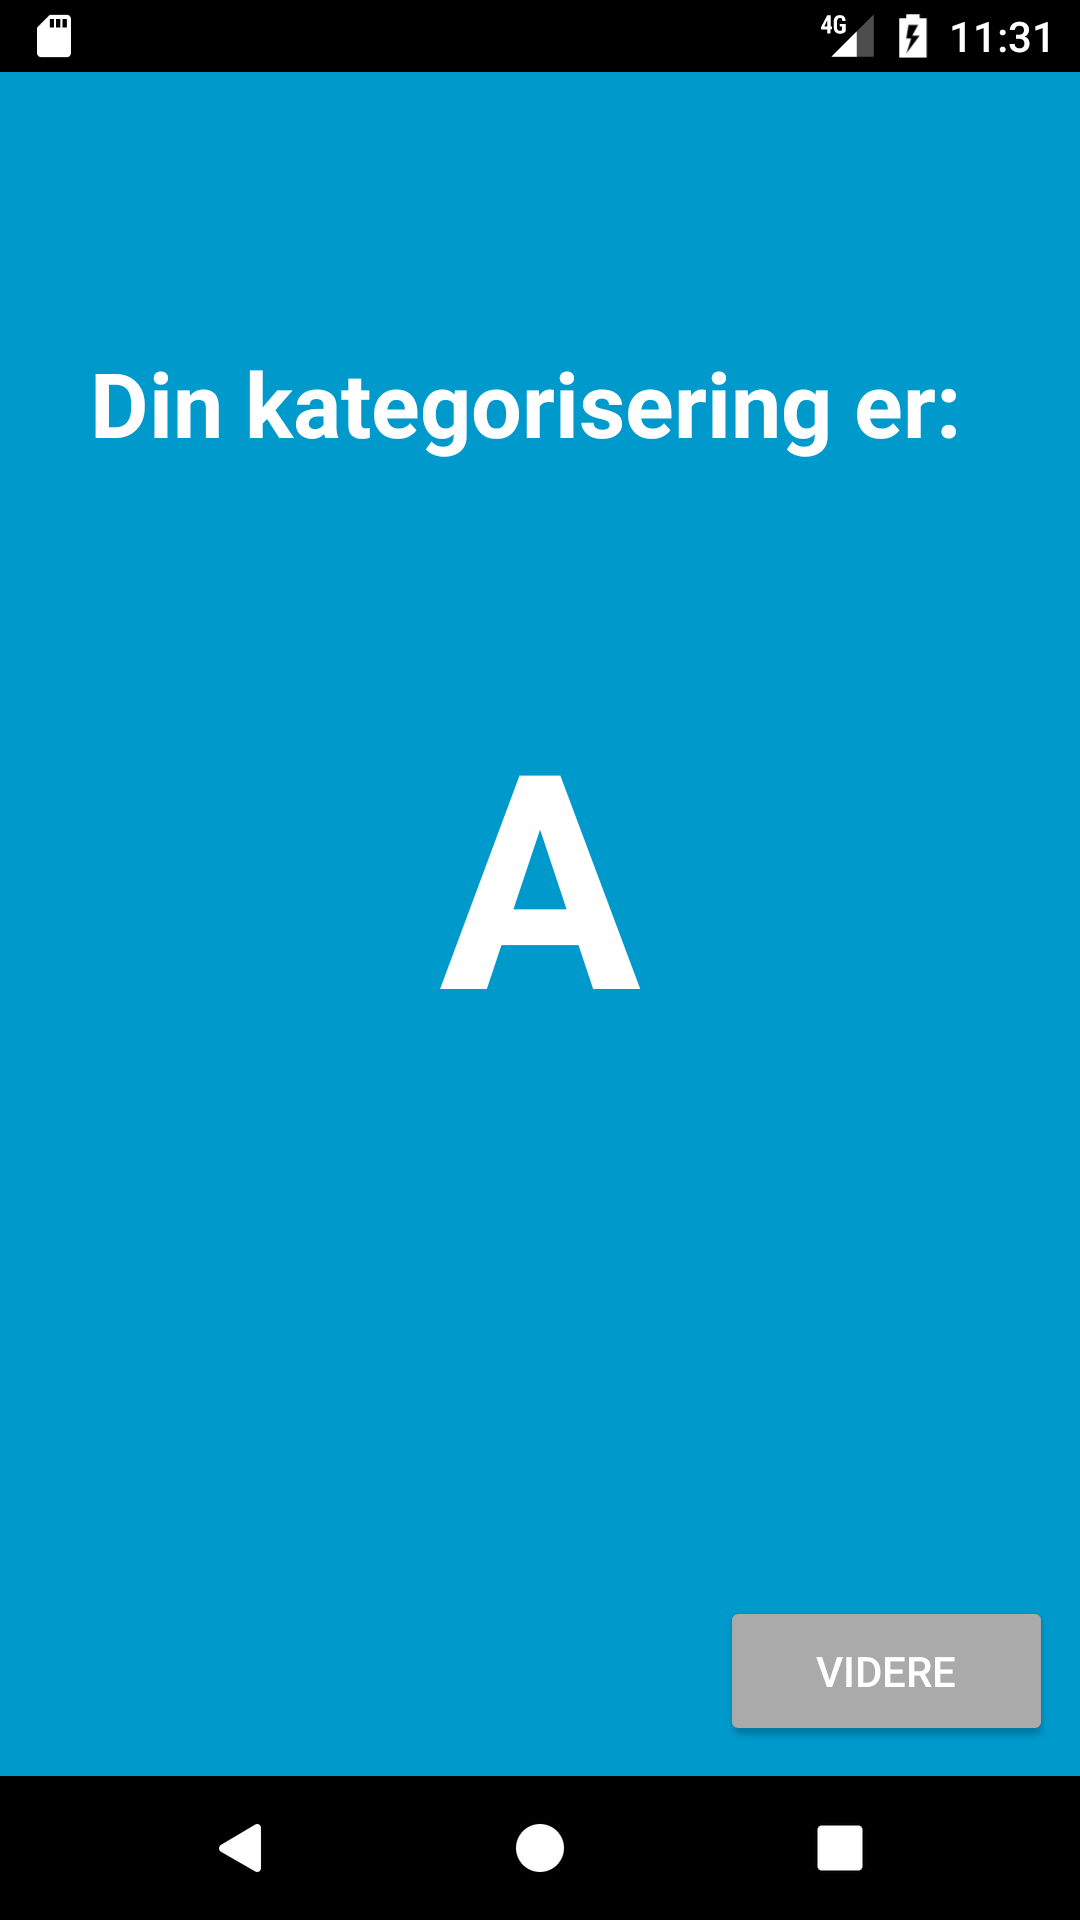
\includegraphics[width=0.24\textwidth, height=60mm]{figures/test/testdatabase}}
  \hspace{5mm}
   \raisebox{-\totalheight}{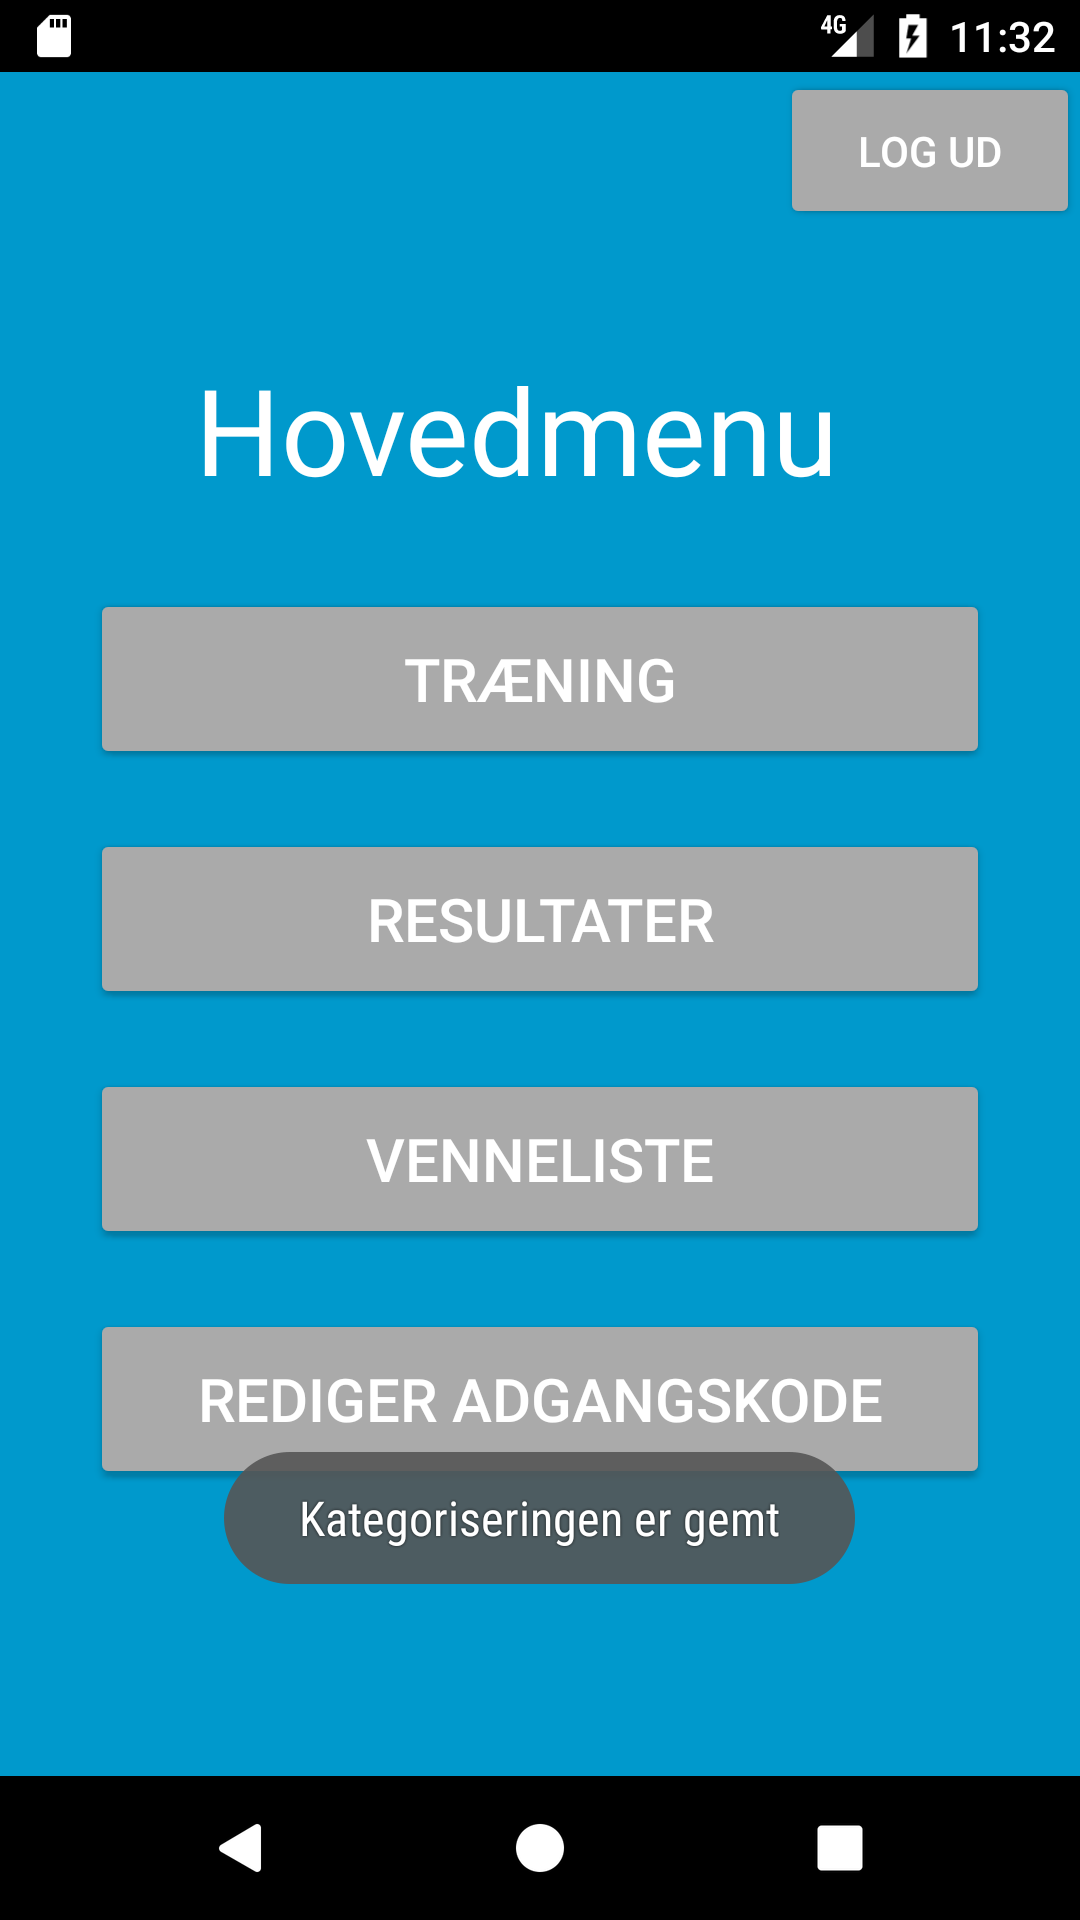
\includegraphics[width=0.24\textwidth, height=60mm]{figures/test/testdatabase1}} 
     \hspace{5mm}
    \raisebox{-\totalheight}{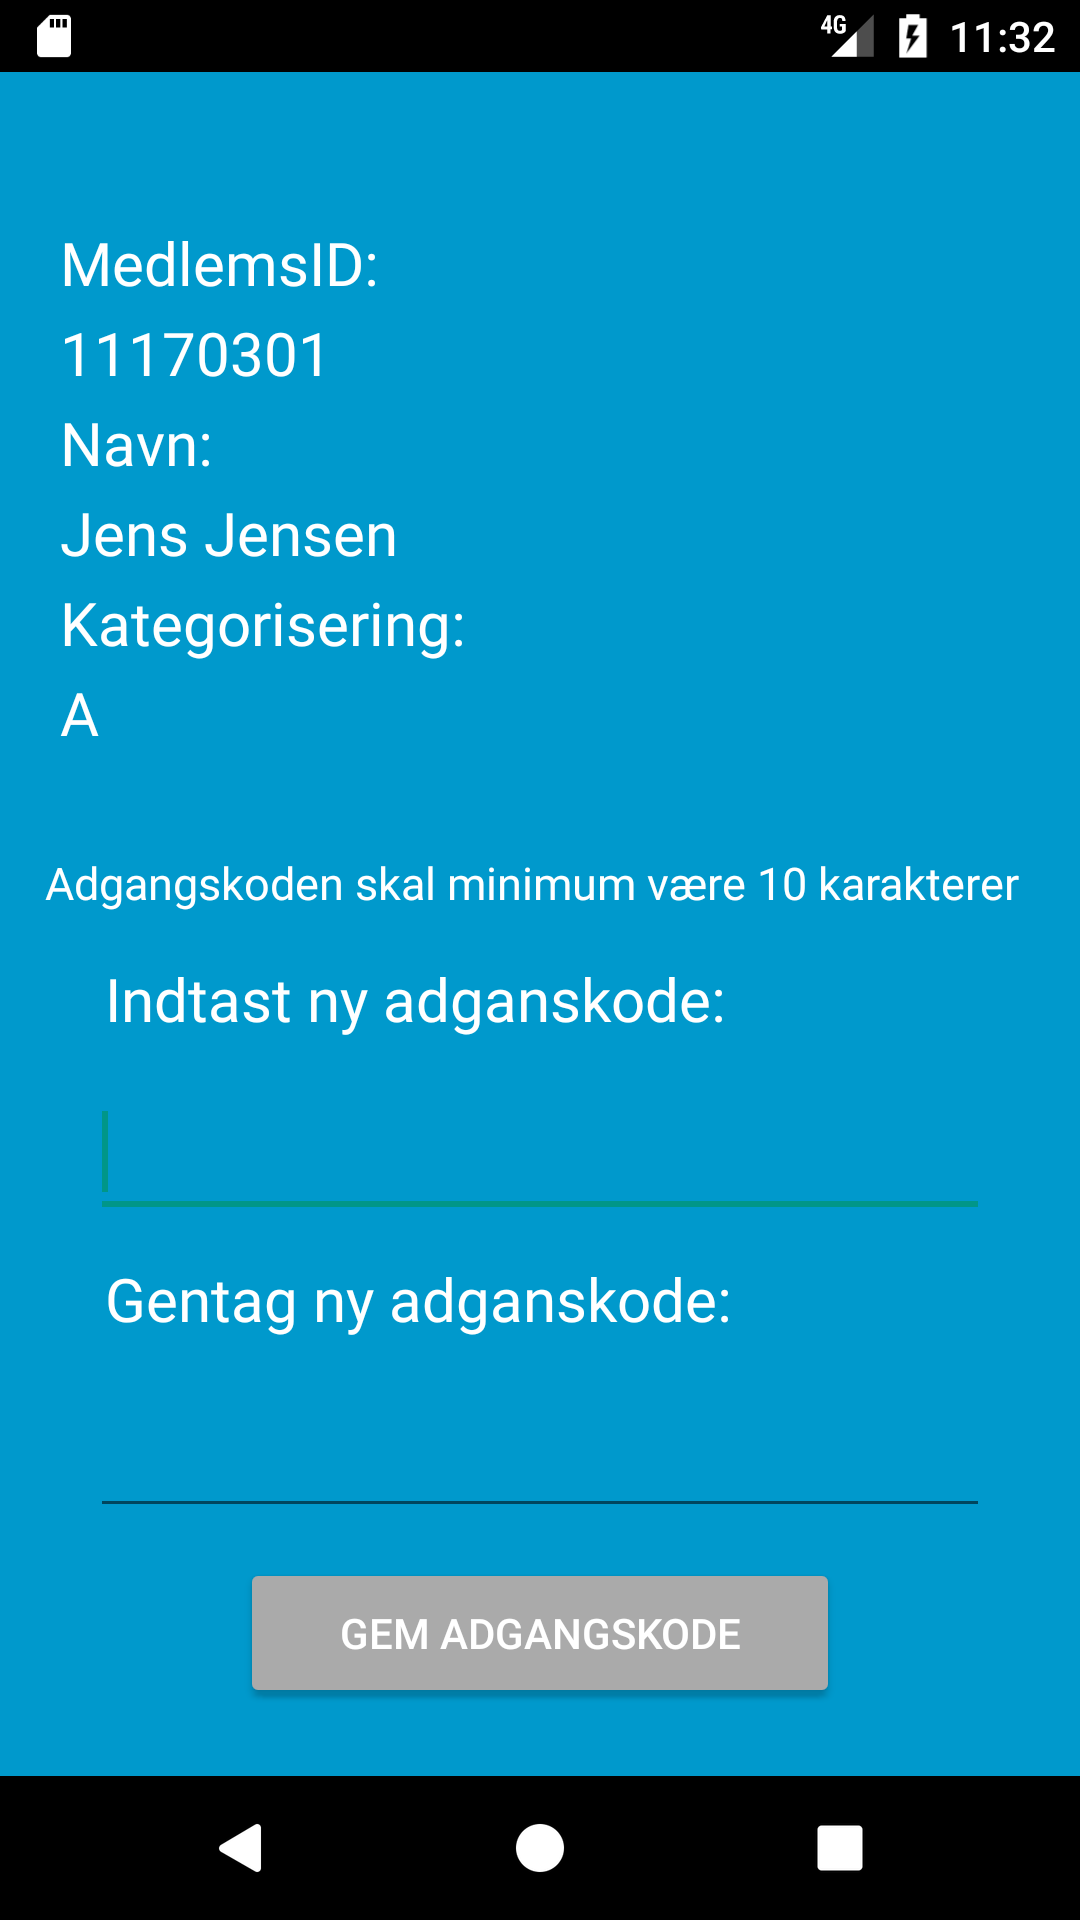
\includegraphics[width=0.24\textwidth, height=60mm]{figures/test/testdatabase2}} 
    \vspace{3mm}
    ~~~~~~~~~~~ \textbf{\textit{Figur 1}}~~~~~~~~~~~~~~~~~~~~~~~~\textbf{\textit{Figur 2}}~~~~~~~~~~~~~~~~~~~~~~~~\textbf{\textit{Figur 3}}
    \newline
Resultater for test af database fremgår af ovenstående figurer. Til venstre er der opnået en kategorisering svarende til A, som på figureren i midten viser, at kategoriseringen er gemt i databasen. Til højre vises redigering af adgangskode, hvor brugeroplysninger om den oprettede bruger, Jens Jensen, vises. Disse værdier er hentet fra databasen, idet brugeren logger ind. Dertil er kategoriseringen opdateret i forhold til den nye kategorisering. 
\begin{itemize}[label={\checkmark}]
 \item På baggrund af denne test er kravene for databasen opfyldt
 \end{itemize}
  \\ \hline
    \caption{Test af database.}
    \label{tab:testDatabase}
\end{longtable}


\section{Log ind}
Log ind anvendes for at adskille brugere, som er registreret i databasen. Derudover er det med til at sikre, at brugeren har deltaget i et rehabiliteringsforløb, da det kun er disse brugere, der bliver registreret i databasen. Der er opstillet funktionelle krav til log ind:

\begin{itemize}
\item Brugere skal kunne logge ind med et personligt medlemsID og adgangskode
\\
\textit{Dette er nødvendigt for at tilgå og sikre, at brugere har deltaget i et rehabiliteringsforløb samt adskille brugeres data}
\end{itemize}

\noindent
Til at teste, hvorvidt kravene til log ind er opfyldt, udføres testen, der fremgår af \autoref{tab:testLogInd}.

  \begin{longtable}{ | l | p{13cm} |} \hline
    \textbf{Test:} & Log ind \\ \hline
     \textbf{Formål:} & Formålet er at teste, hvorvidt log ind-funktionen i systemet opfylder krav opstillet til log ind. Dette gøres ved at logge ind med en bruger, der findes i databasen og en bruger, som ikke findes i databasen. 
 \\ \hline
 	\textbf{Main flow:} & 1.~Indtast et medlemsID, som ikke eksisterer i databasen \textit{123456} og en adgangskode, som eksisterer i databasen \textit{adgangskode} og tryk på log ind knappen.
 	\begin{itemize}
 	\item Log ind mislykkedes. Fejlmeddelelse vises i grænsefladen for log ind (\textbf{\textit{Figur 1}})
 	\end{itemize}
2.~Indtast et MedlemsID, som eksisterer i databasen \textit{11170301} og en adgangskode, som ikke tilhører medlemsID’et \textit{forkertadgangskode} og tryk på log ind-knappen.
 \begin{itemize}
 \item Log ind mislykkedes. Fejlmeddelelse vises i grænsefladen for log ind (\textbf{\textit{Figur 2}})
 \end{itemize}
3.~Indtast et medlemsID \textit{11170301} og en adgangskode \textit{adgangskode}, som eksisterer i databasen. 
\begin{itemize}
\item Log ind lykkedes og hovedmenu vises (\textbf{\textit{Figur 3}})
\end{itemize}
 \\  \hline
 \textbf{Resultat:} &  \hspace{1.5mm}
  \raisebox{-\totalheight}{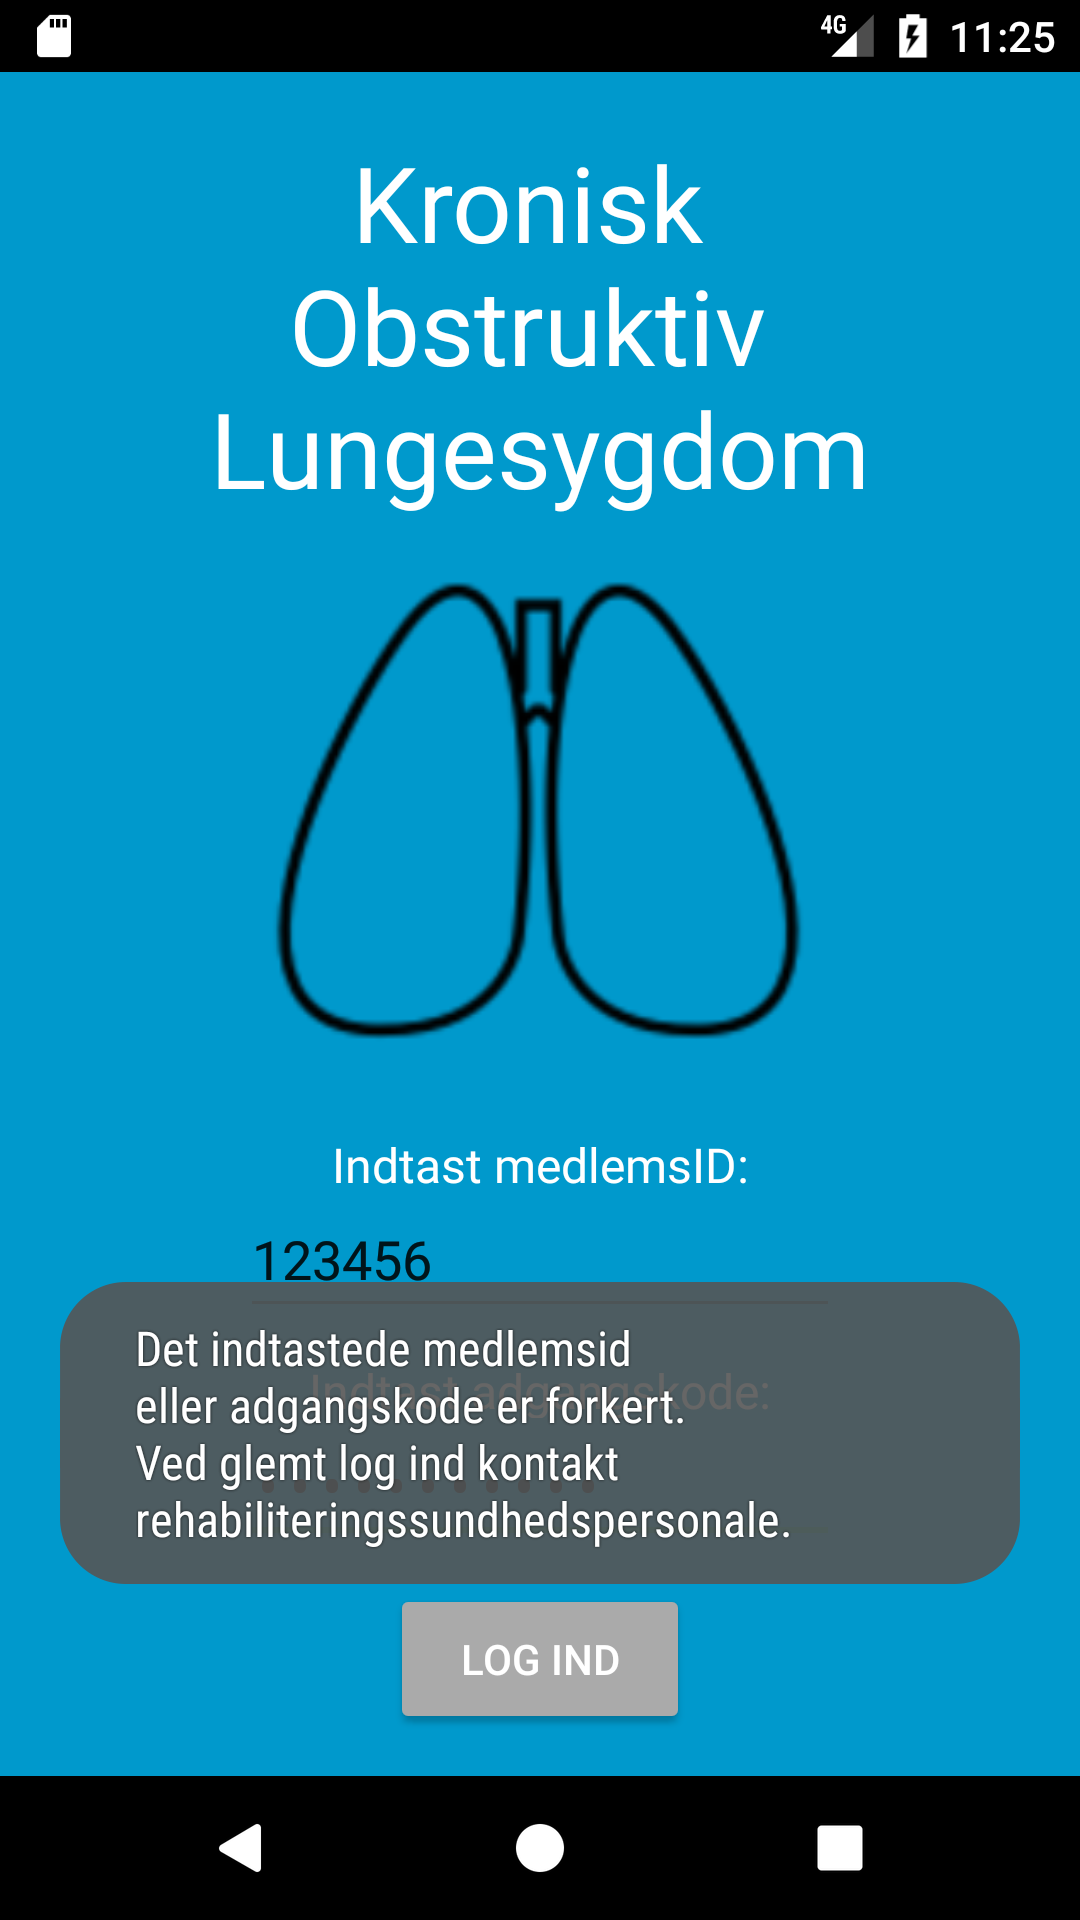
\includegraphics[width=0.24\textwidth, height=60mm]{figures/test/testlogind1}} 
  \hspace{5mm}
   \raisebox{-\totalheight}{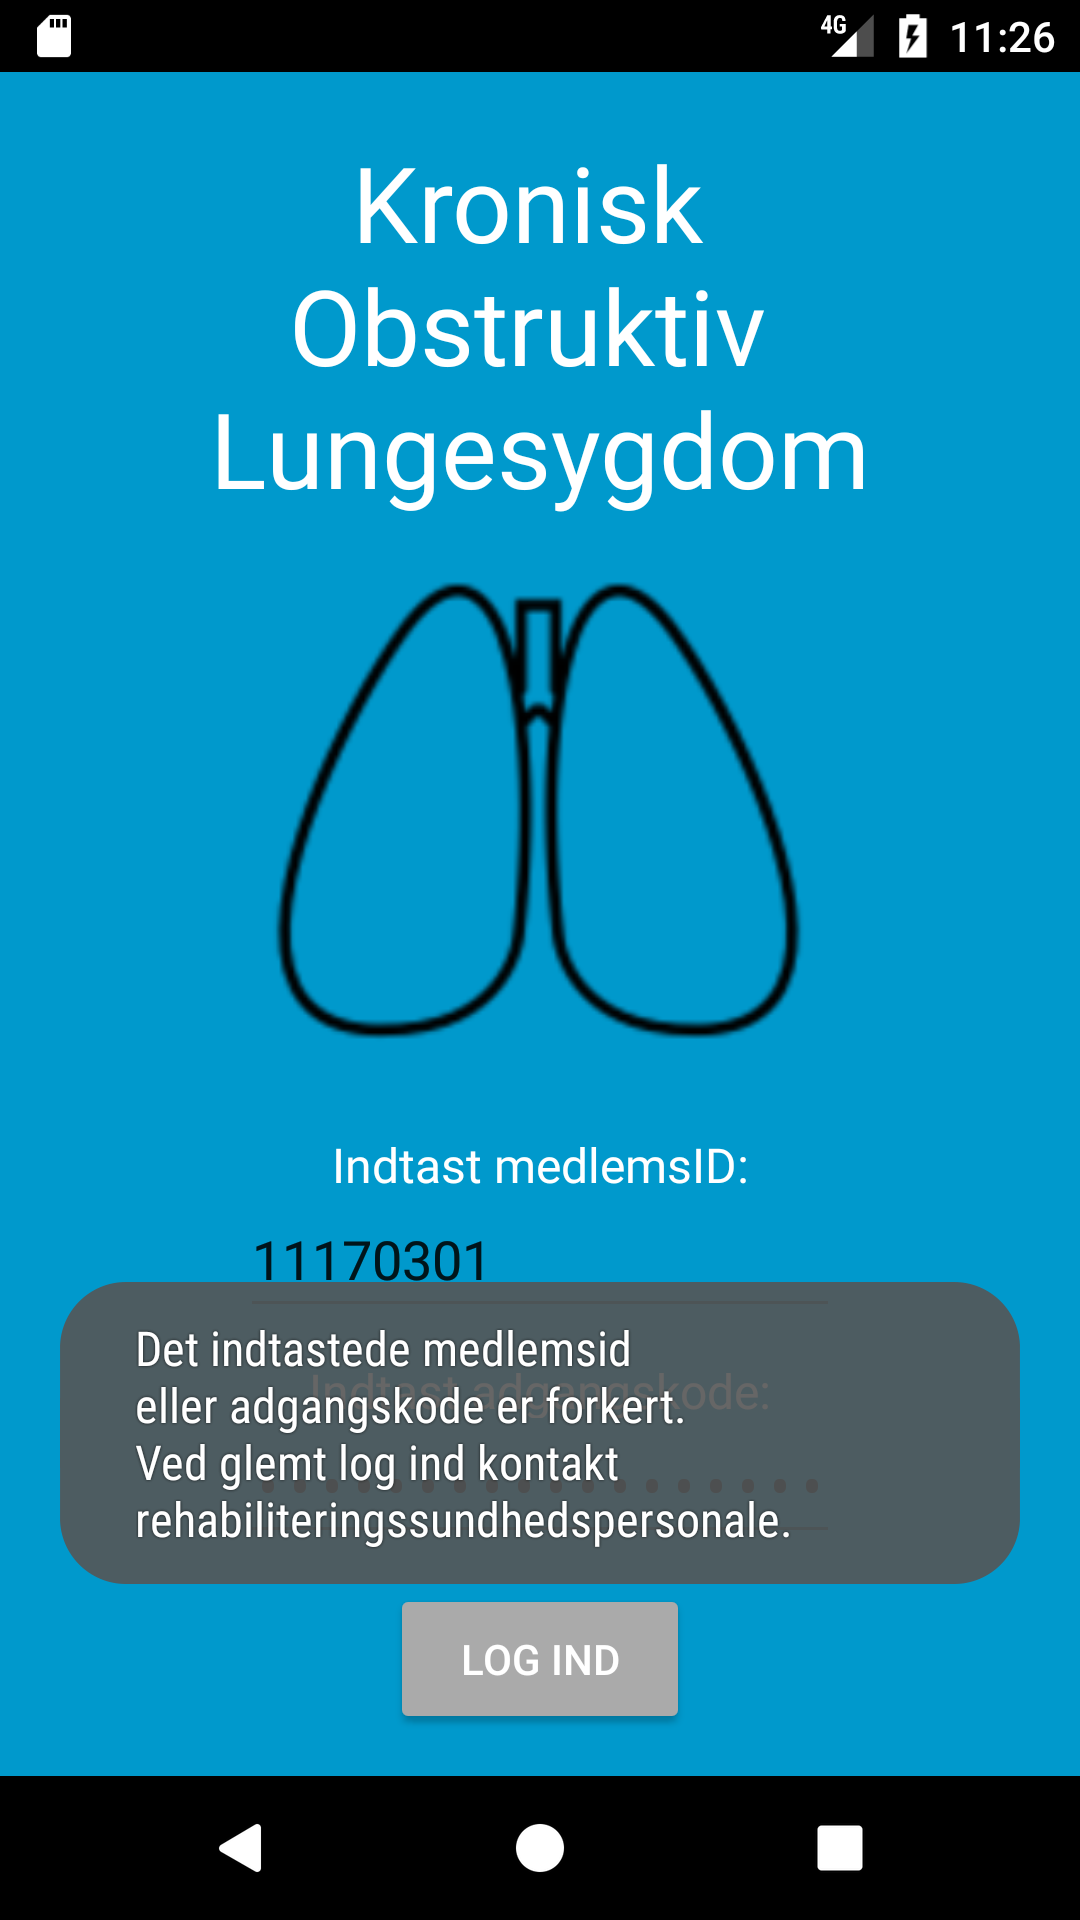
\includegraphics[width=0.24\textwidth, height=60mm]{figures/test/testlogind}} 
     \hspace{5mm}
    \raisebox{-\totalheight}{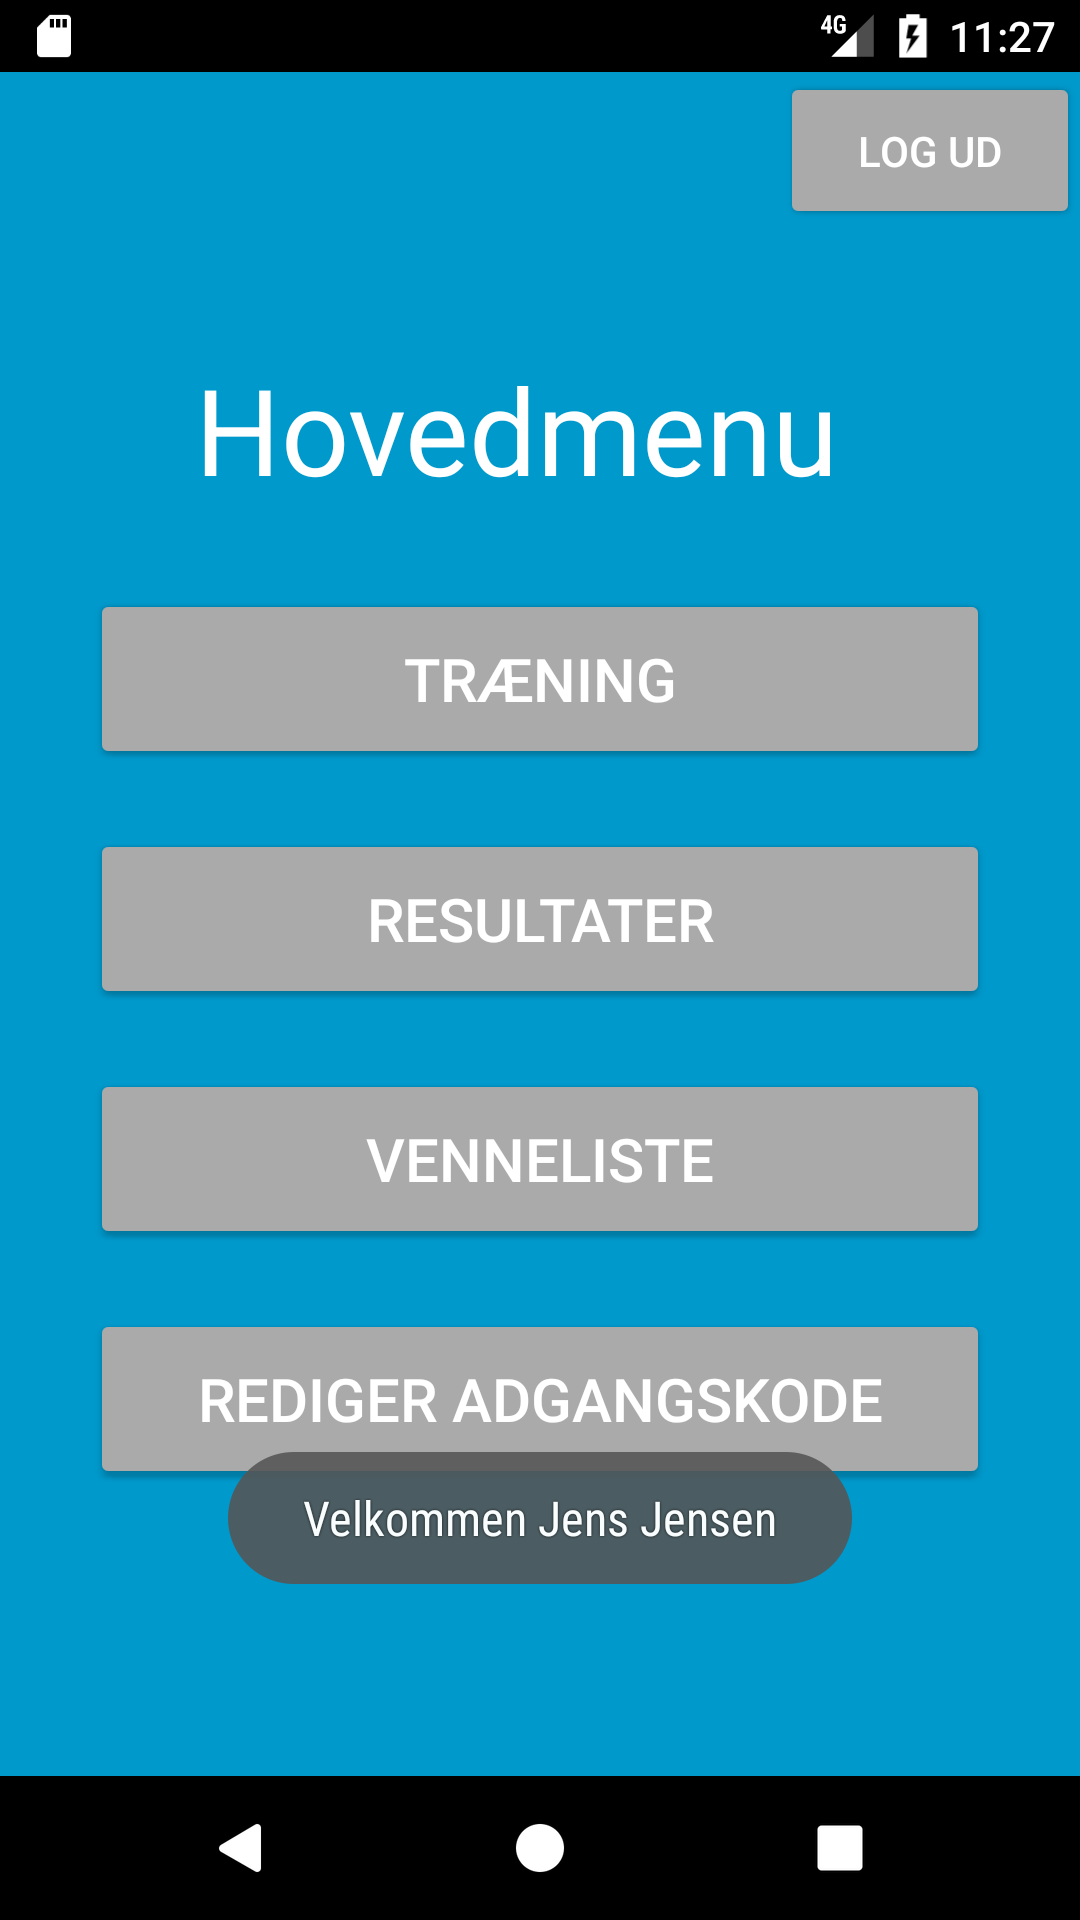
\includegraphics[width=0.24\textwidth, height=60mm]{figures/test/testlogind2}} 
    \vspace{3mm}
       ~~~~~~~~~~~ \textbf{\textit{Figur 1}}~~~~~~~~~~~~~~~~~~~~~~~~\textbf{\textit{Figur 2}}~~~~~~~~~~~~~~~~~~~~~~~~\textbf{\textit{Figur 3}}
    \newline
Resultater for test af log ind fremgår af ovenstående figurer. Til venstre og i midten testes der for henholdsvis første og andet main flow. Hertil fremgår det, at log ind mislykkedes, hvoraf fejlmeddelelsen vises. Til højre fremgår det, at log ind lykkedes, og hovedmenuen vises.  
\begin{itemize}[label={\checkmark}]
 \item På baggrund af denne test er kravet for log ind opfyldt
 \end{itemize}
 \\ \hline
    \caption{Test af Log ind.}
    \label{tab:testLogInd}
\end{longtable}

\section{Kategorisering}
Kategoriseringen skal foretages første gang brugeren logger ind i app'en og skal være en parameter i tilpasningen af et træningsniveau for den enkelte bruger. Følgende krav blev opstillet til kategoriseringen:

\begin{itemize}
\item Systemet skal kunne kategorisere brugere i ABCD på baggrund af CAT-score og antallet af årlige indlæggelser på grund af KOL
\\
\textit{Dette er nødvendigt for at kunne tilpasse træningen efter den enkelte bruger}
\end{itemize}

\noindent
Det testes, om de opstillede krav til kategorisering er overholdt. Testen fremgår af \autoref{tab:testKategorisering}.

  \begin{longtable}{ | l | p{13cm} |} \hline
    \textbf{Test:} & Kategorisering  \\ \hline
     \textbf{Formål:} & Formålet er, at systemet skal kunne kategorisere brugere i ABCD efter, at  brugeren har svaret på udsagn fra CAT-score og angivet antallet af indlæggelser forårsaget af KOL inden for det seneste år. Dette gøres ved at angive forskellige værdier, der giver kategorisering A, B, C, eller D.
 \\ \hline
 	\textbf{Main flow:} & 1.~Få en samlet CAT-score under 10. Vælg \textit{0,1,2,1,0,1,0,1}, tryk videre efter hver angivet værdi og vælg til sidst antal indlæggelser \textit{0 INDLÆGGELSER}. 
 	\begin{itemize} 
 	\item Kategorisering er A (\textbf{\textit{Figur 4}})
 	\end{itemize}	
 	2.~Få en samlet CAT-score over 10. \textit{5,1,2,3,4,5,1,5}, tryk videre efter hver angivet værdi og vælg til sidst antal indlæggelser \textit{0 INDLÆGGELSER}.
 	\begin{itemize}
 	\item Kategorisering er B (\textbf{\textit{Figur 5}})
 	\end{itemize}
3.~Få en samlet CAT-score under 10. \textit{0,1,2,1,0,1,0,1}, tryk videre efter hver angivet værdi og vælg til sidst antal indlæggelser \textit{1 ELLER FLERE INDLÆGGELSER}.
 \begin{itemize}
  \item Kategorisering er C (\textbf{\textit{Figur 6}})
  \end{itemize}
4.~Få en samlet CAT-score over 10. \textit{5,1,2,3,4,5,1,5}, tryk videre efter hver angivet værdi og vælg til sidst antal indlæggelser \textit{1 ELLER FLERE INDLÆGGELSER}.
\begin{itemize}
\item Kategorisering er D (\textbf{\textit{Figur 7}})
\end{itemize}   \\ \hline
 \textbf{Resultat:} &\hspace{1.5mm}
  \raisebox{-\totalheight}{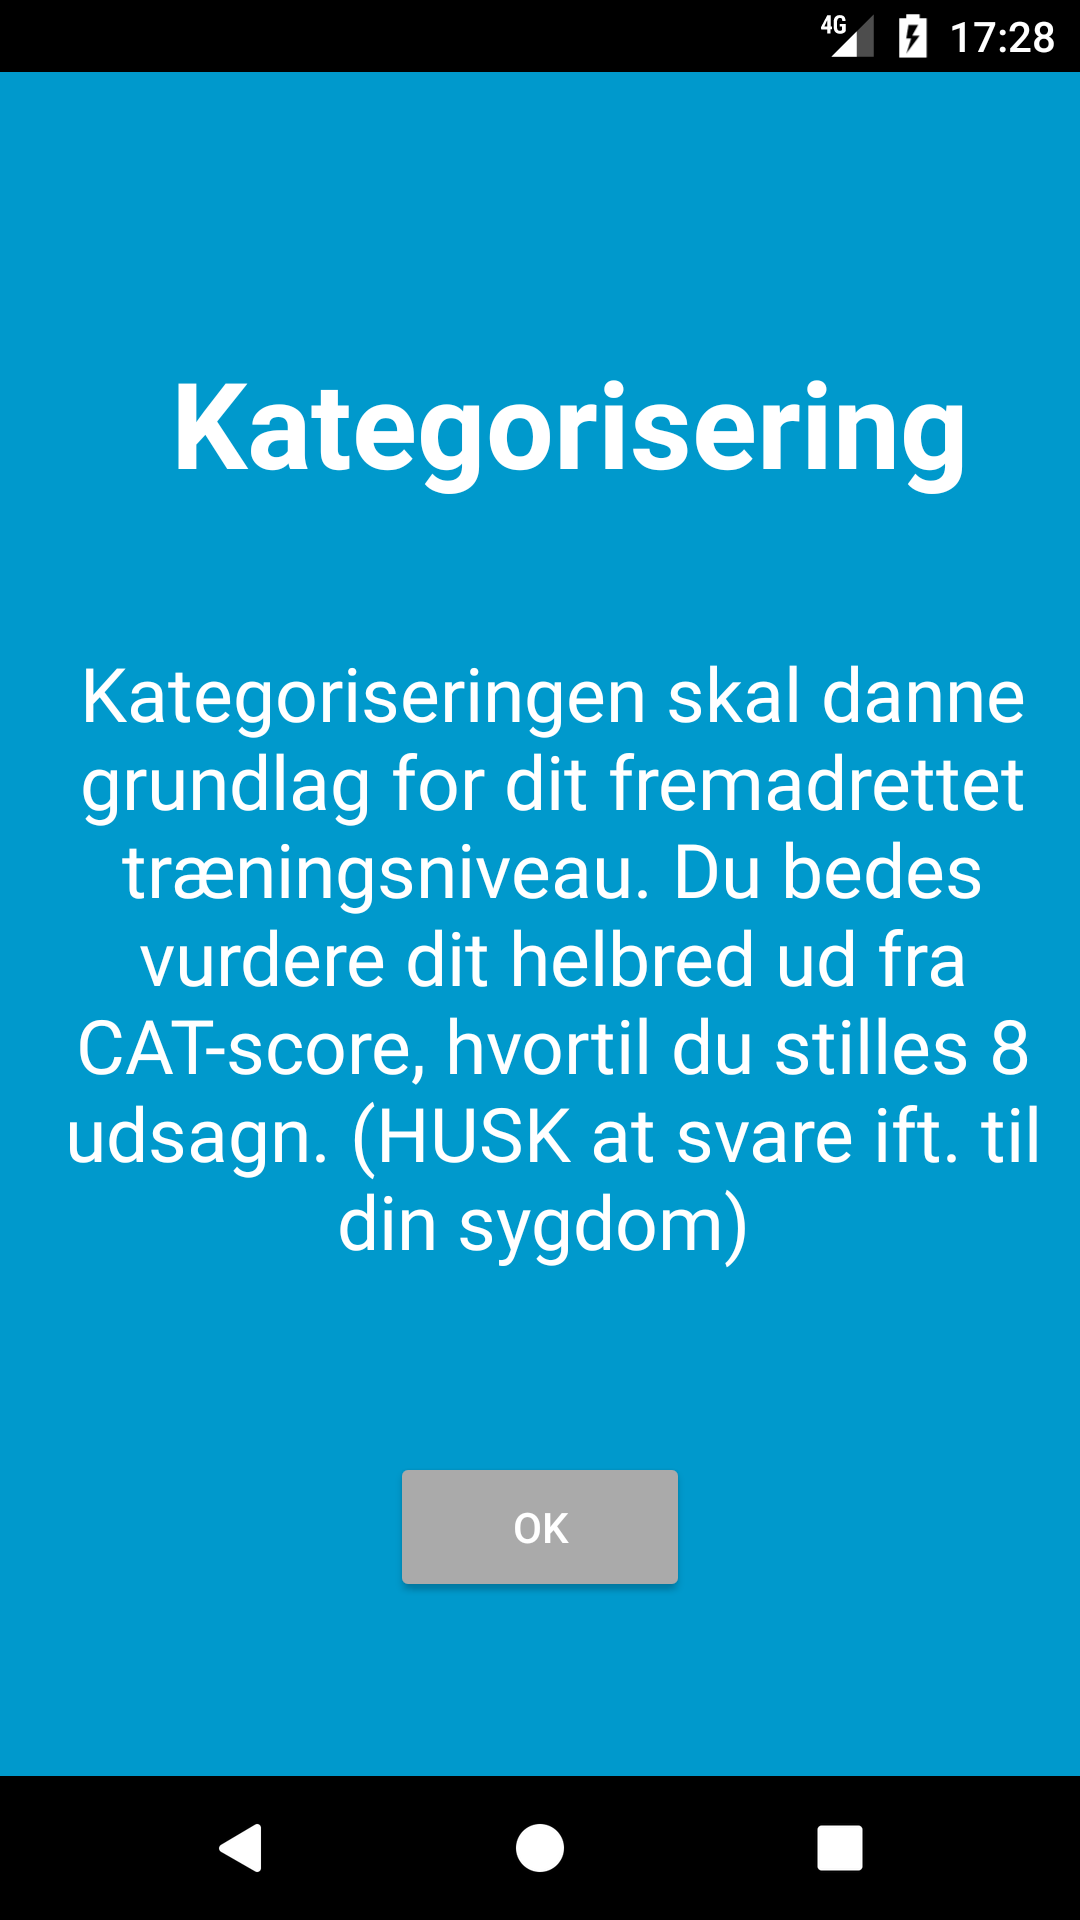
\includegraphics[width=0.24\textwidth, height=60mm]{figures/test/KAT}} 
  \hspace{5mm}
   \raisebox{-\totalheight}{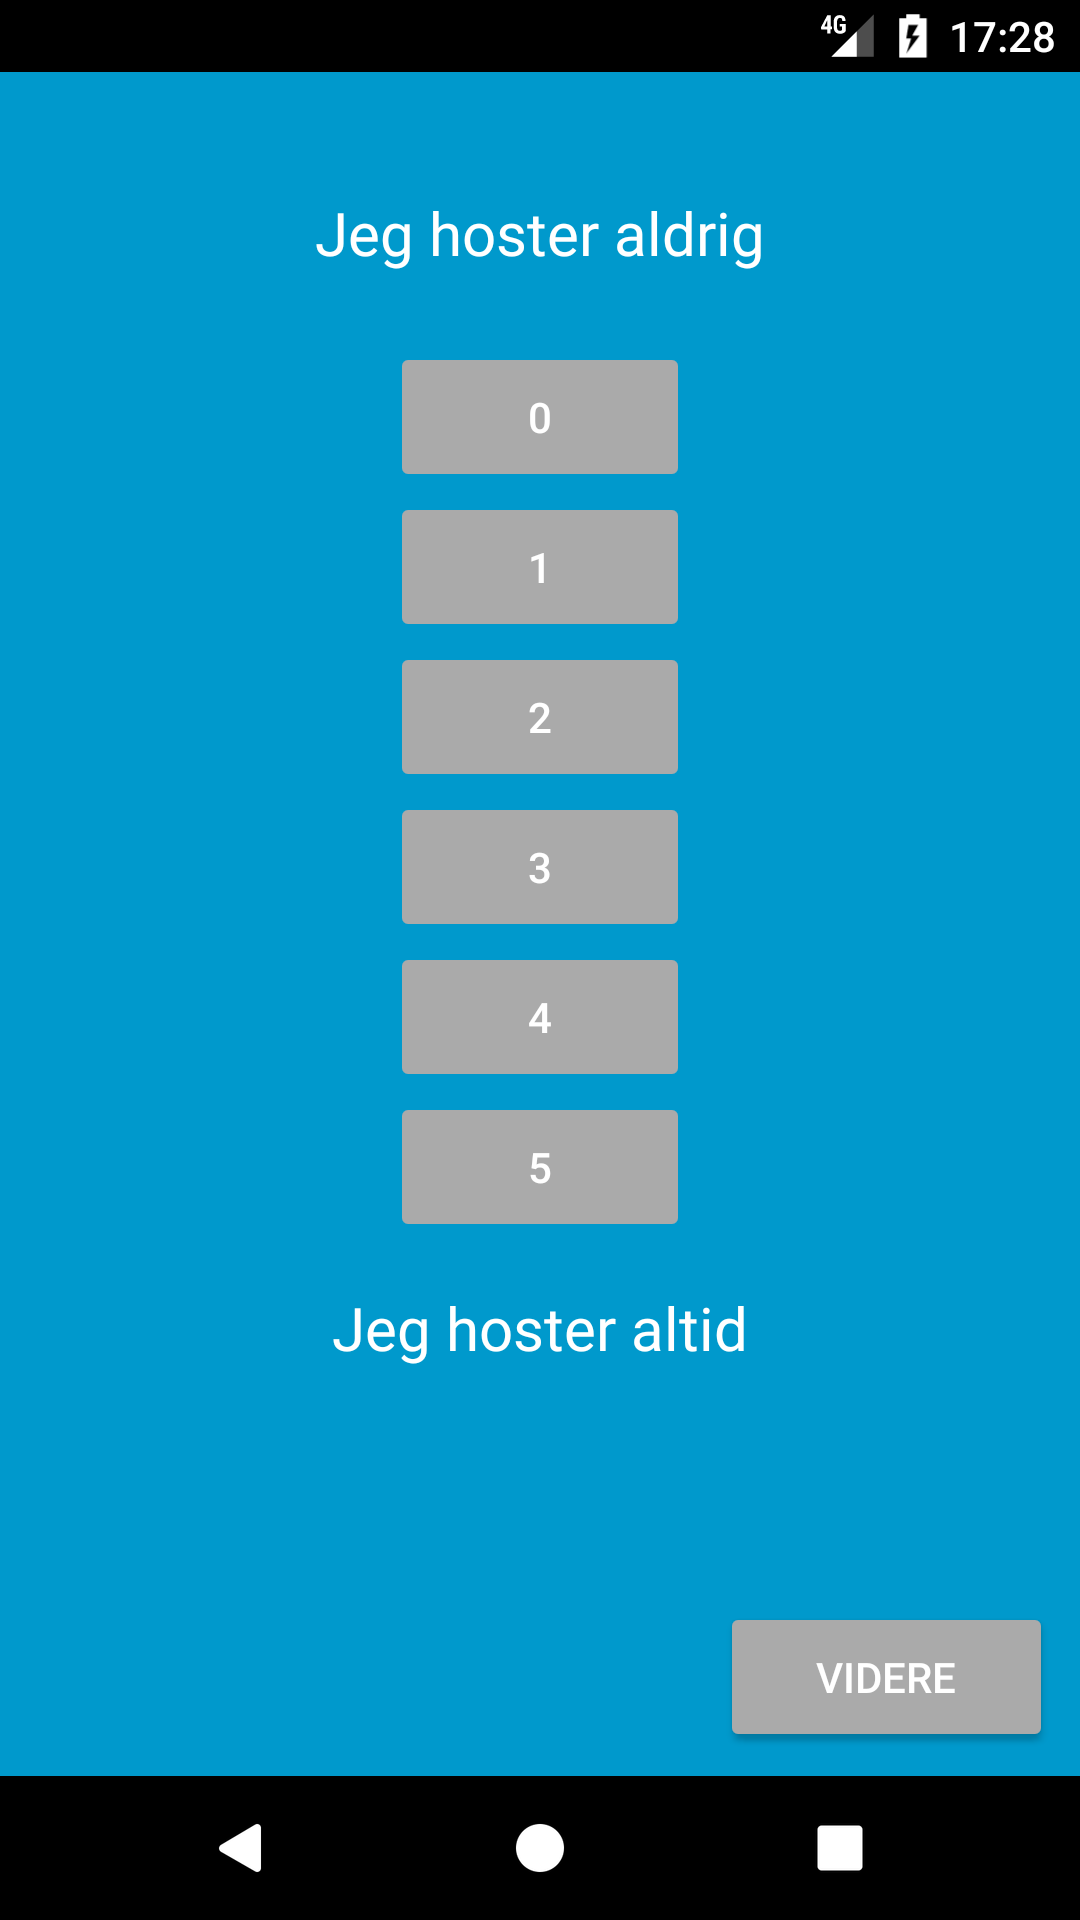
\includegraphics[width=0.24\textwidth, height=60mm]{figures/test/KAT1}} 
     \hspace{5mm}
    \raisebox{-\totalheight}{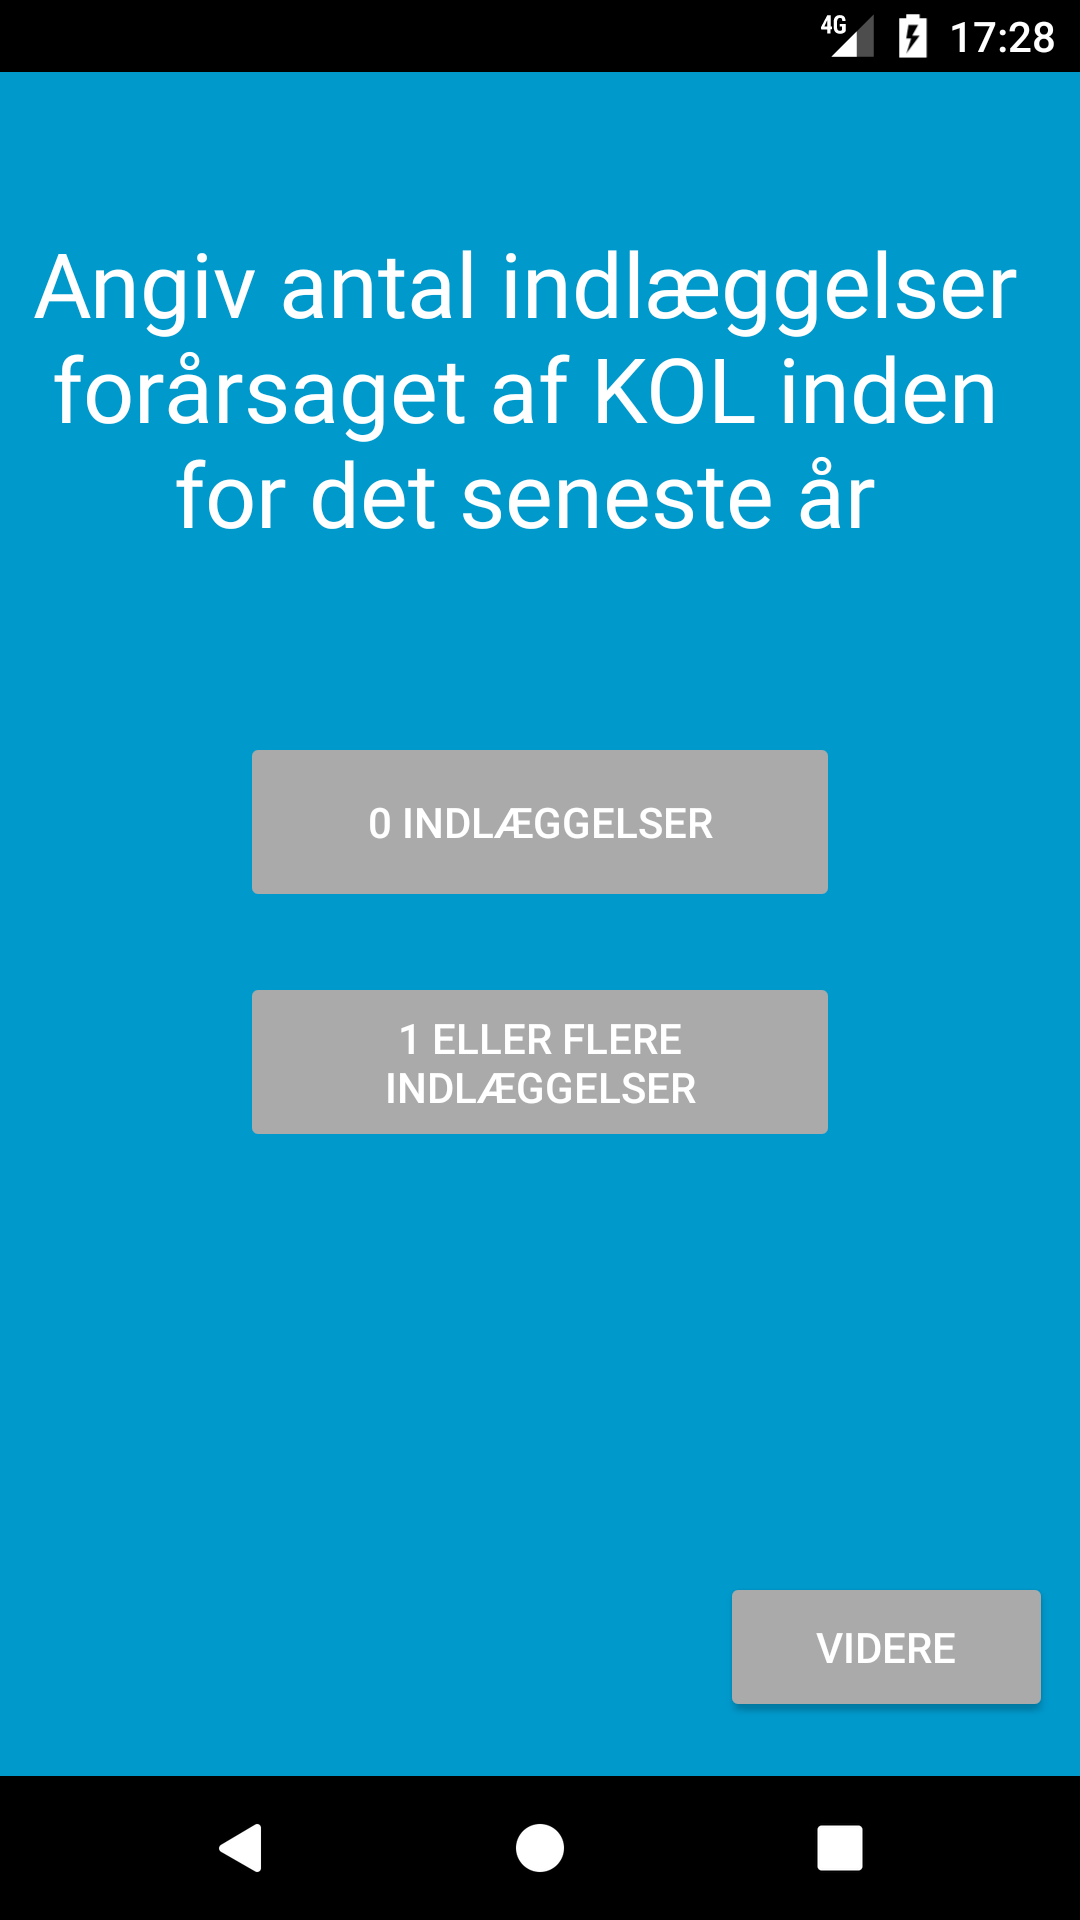
\includegraphics[width=0.24\textwidth, height=60mm]{figures/test/KAT2}} 
    \vspace{3mm}
          ~~~~~~~~~~~ \textbf{\textit{Figur 1}}~~~~~~~~~~~~~~~~~~~~~~~~\textbf{\textit{Figur 2}}~~~~~~~~~~~~~~~~~~~~~~~~\textbf{\textit{Figur 3}}
           \newline
Ovenstående figurer viser grænsefladerne for introduktion til kategorisering, CAT-score og antal indlæggelser. Den midterste figur viser et af de otte udsagn, der udgør CAT-scoren. Disse grænseflader vises før grænsefladen for ABCD-kategorisering.   
 \\ \hline
\textbf{} & \hspace{0.3mm}
  \raisebox{-\totalheight}{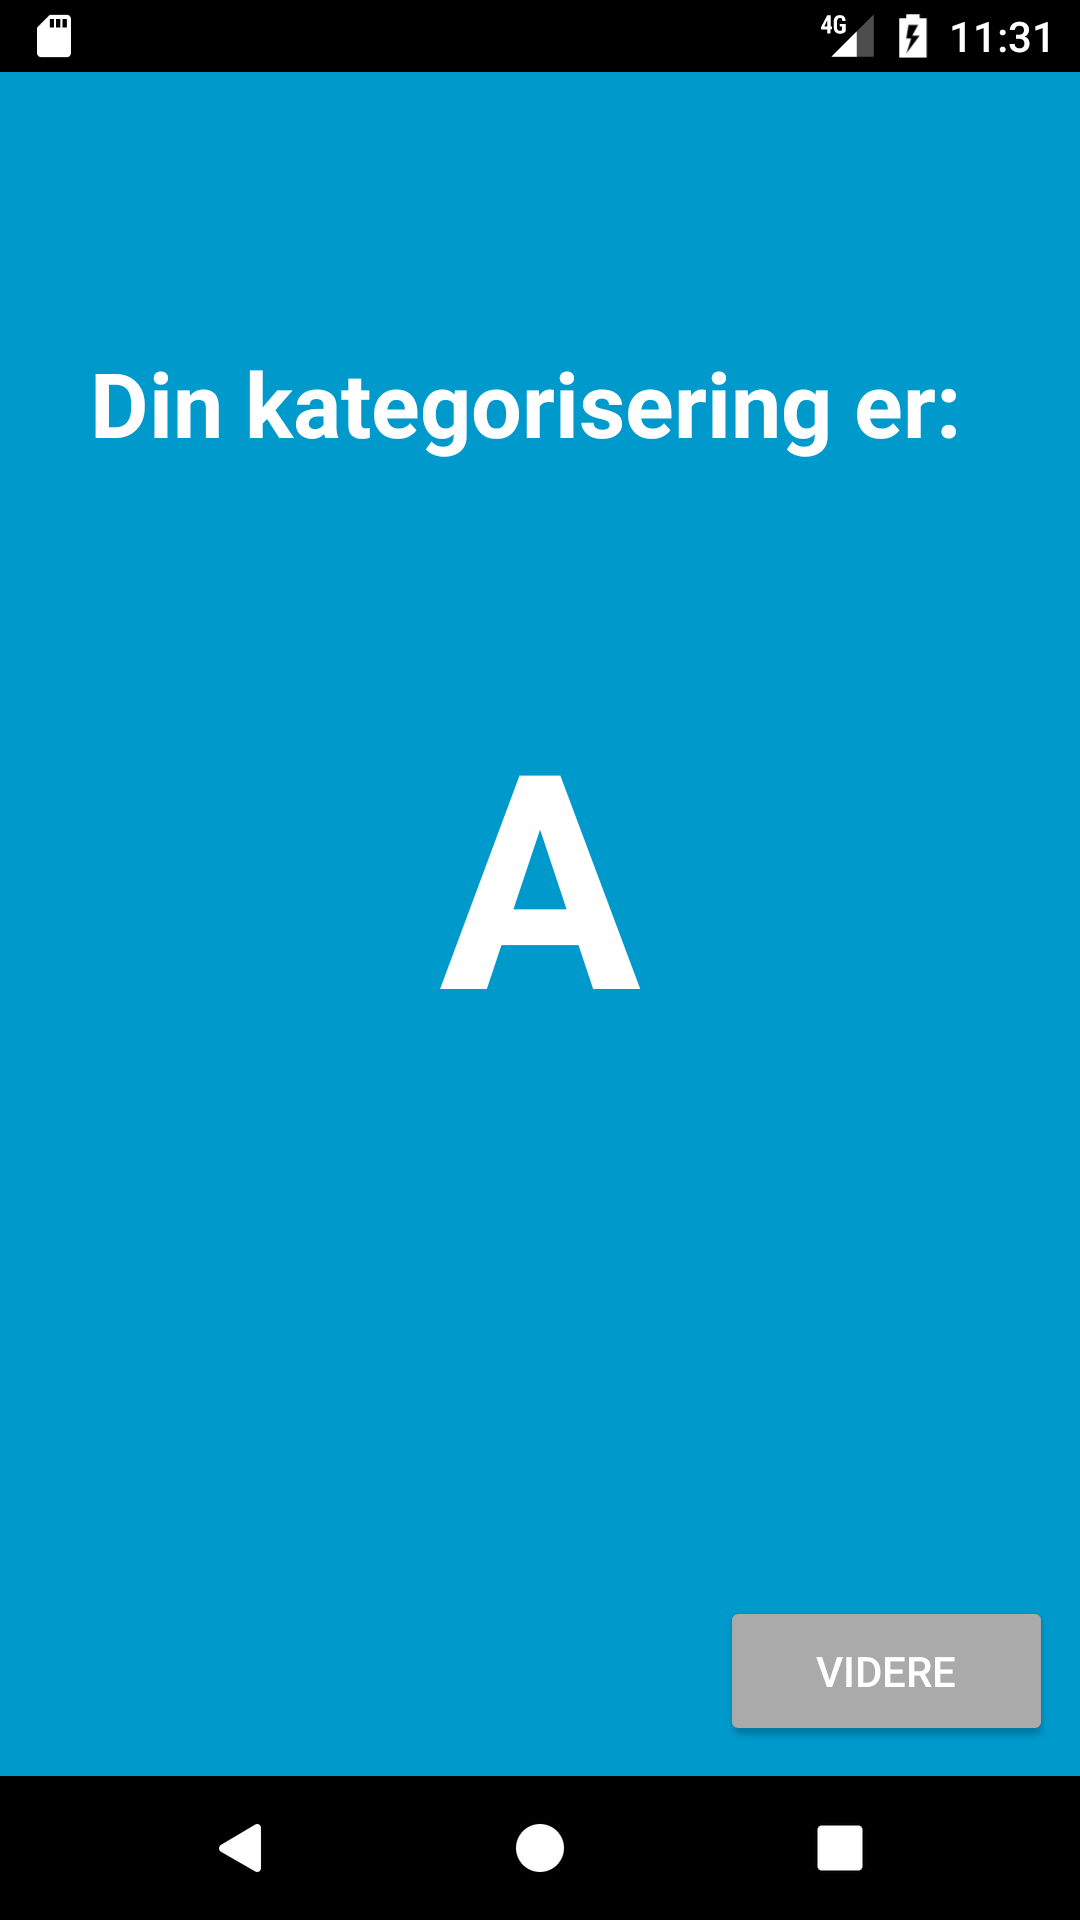
\includegraphics[width=0.20\textwidth, height=60mm]{figures/test/testkat1}} 
   \raisebox{-\totalheight}{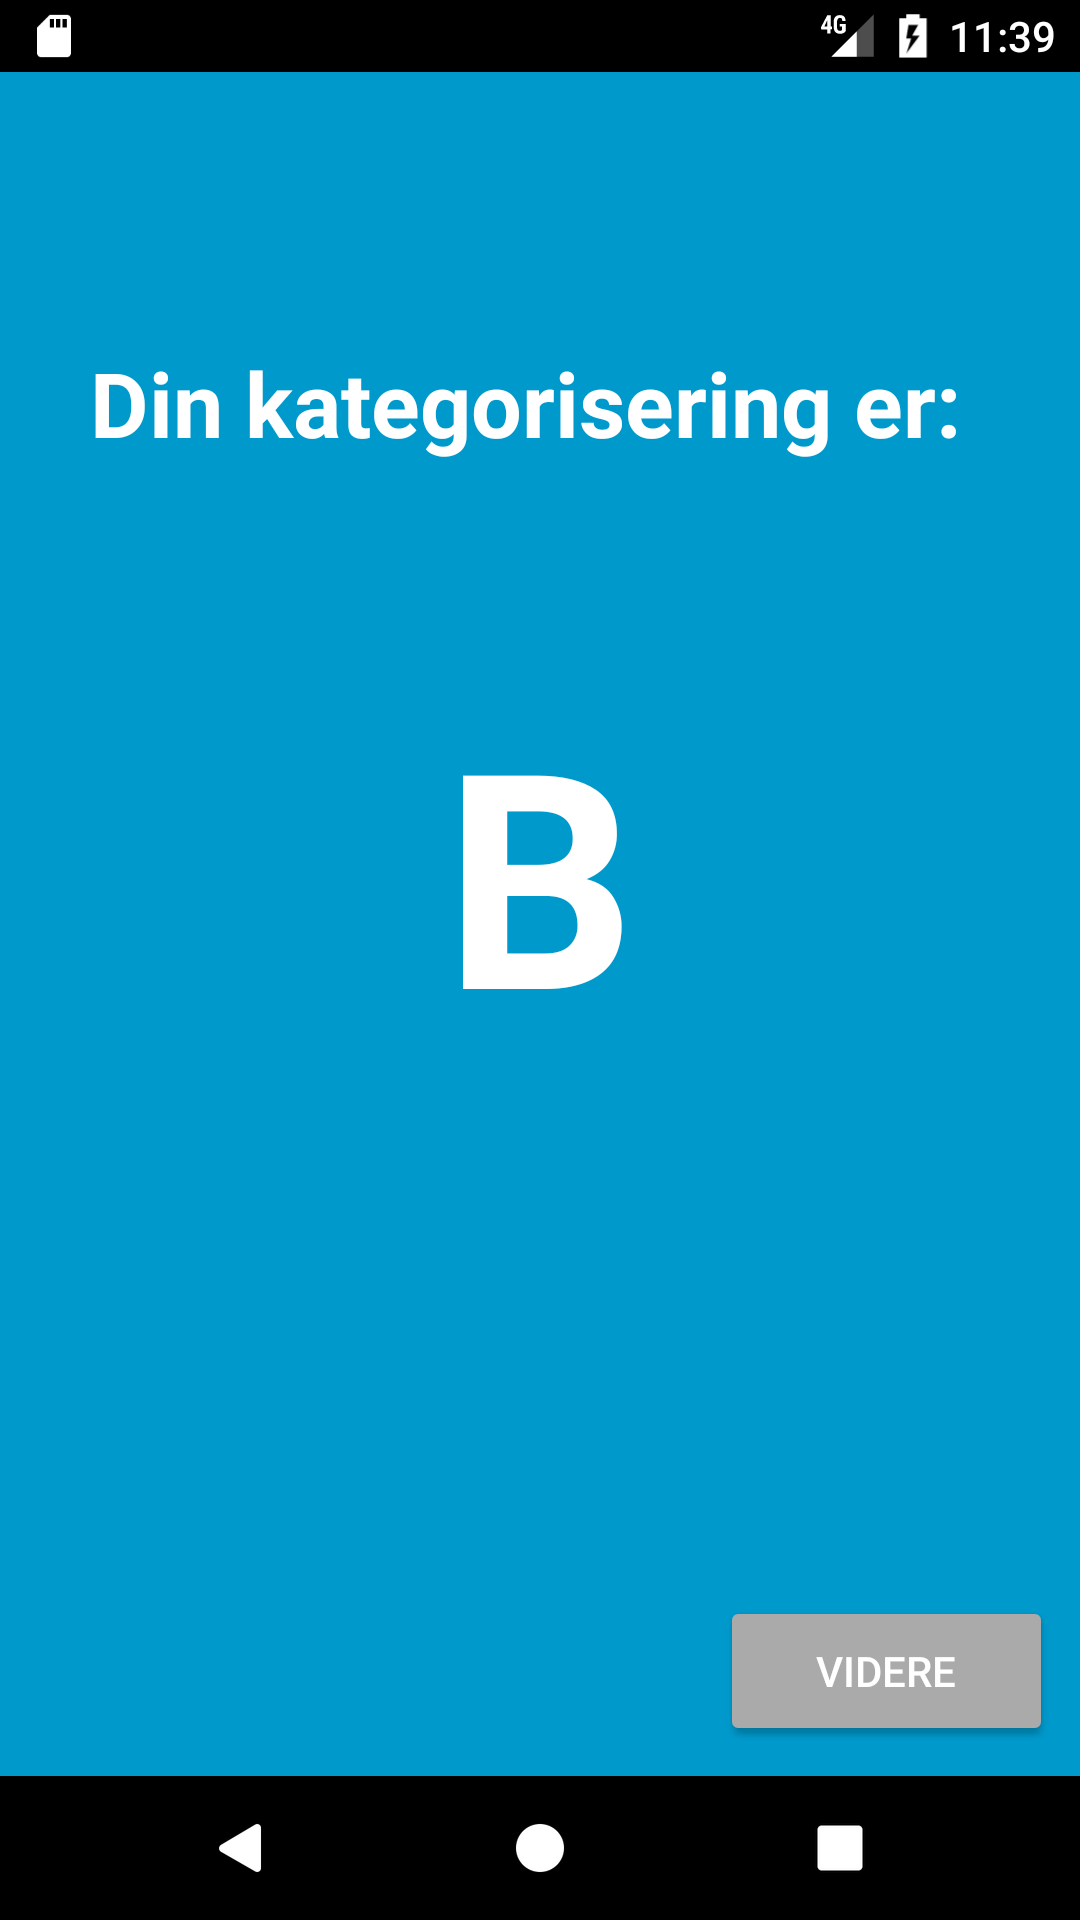
\includegraphics[width=0.20\textwidth, height=60mm]{figures/test/testkat2}} 
    \raisebox{-\totalheight}{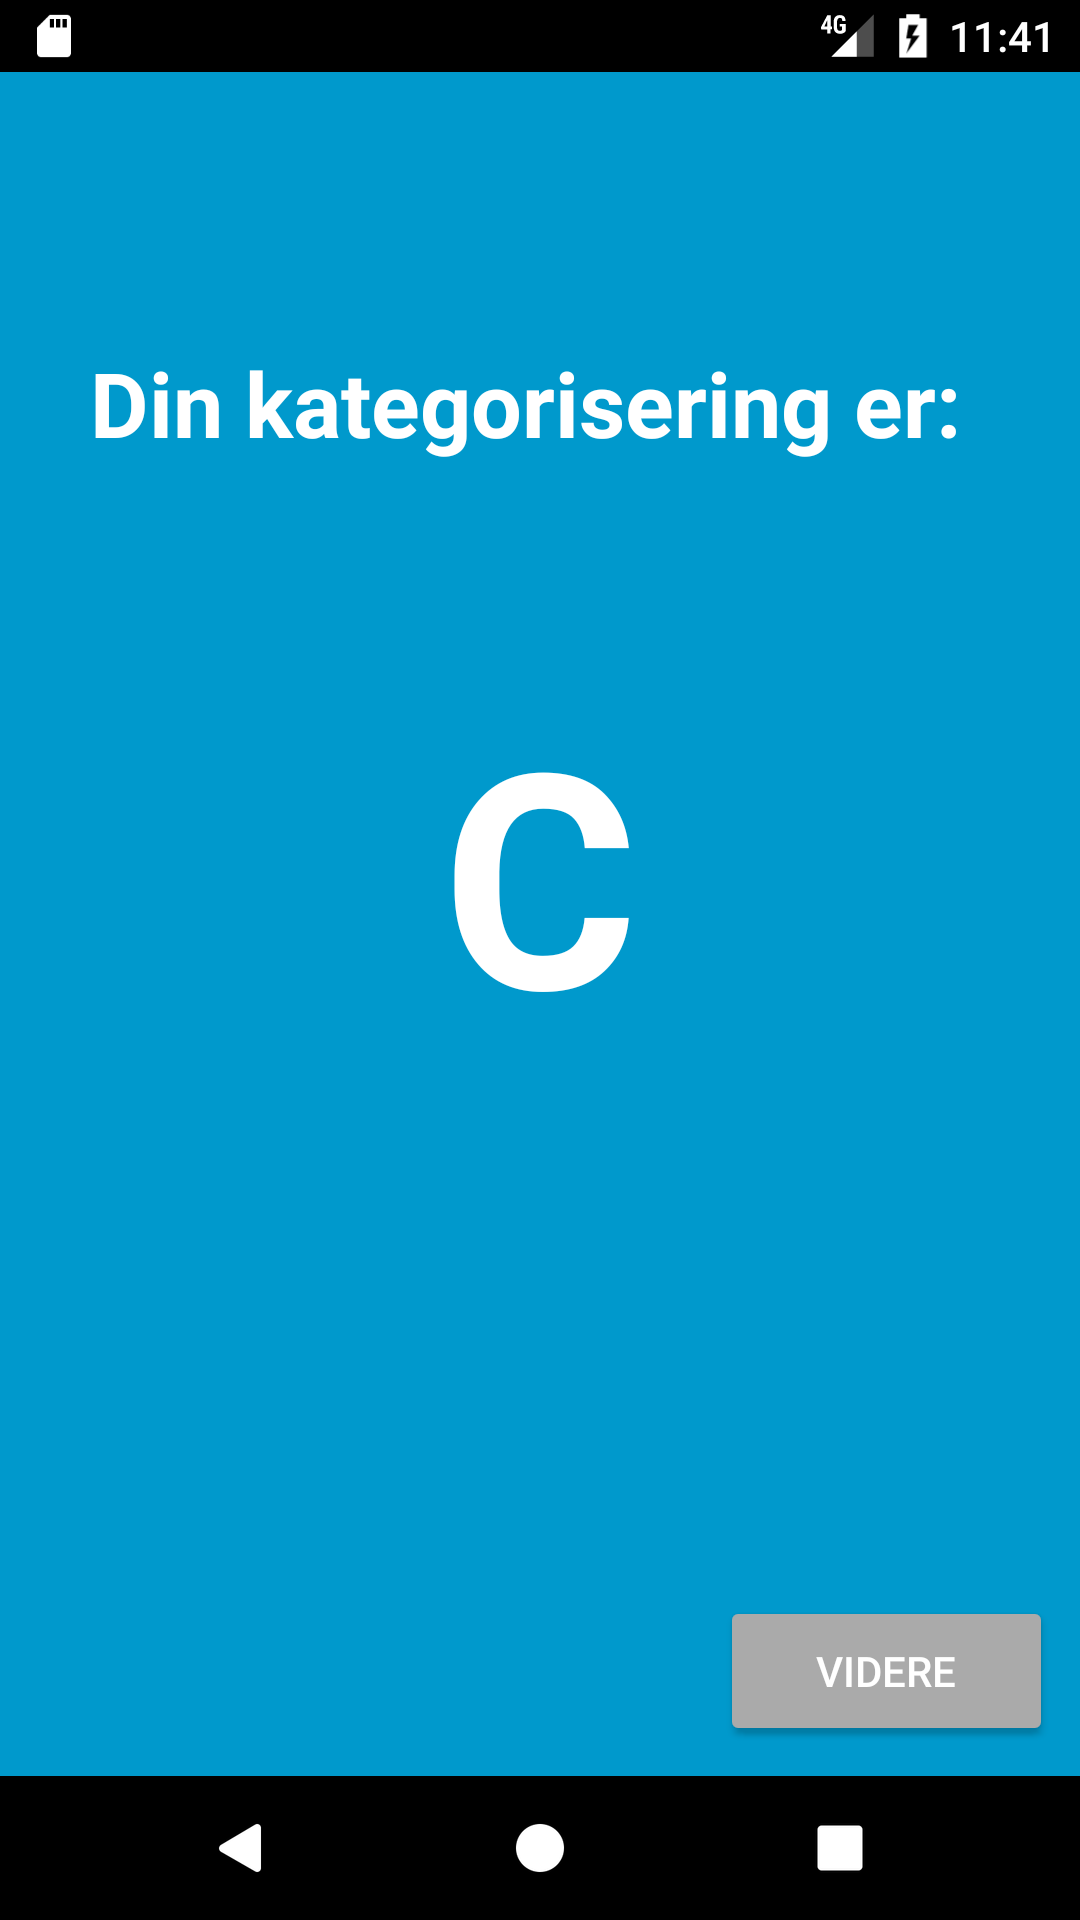
\includegraphics[width=0.20\textwidth, height=60mm]{figures/test/testkat}} 
 \raisebox{-\totalheight}{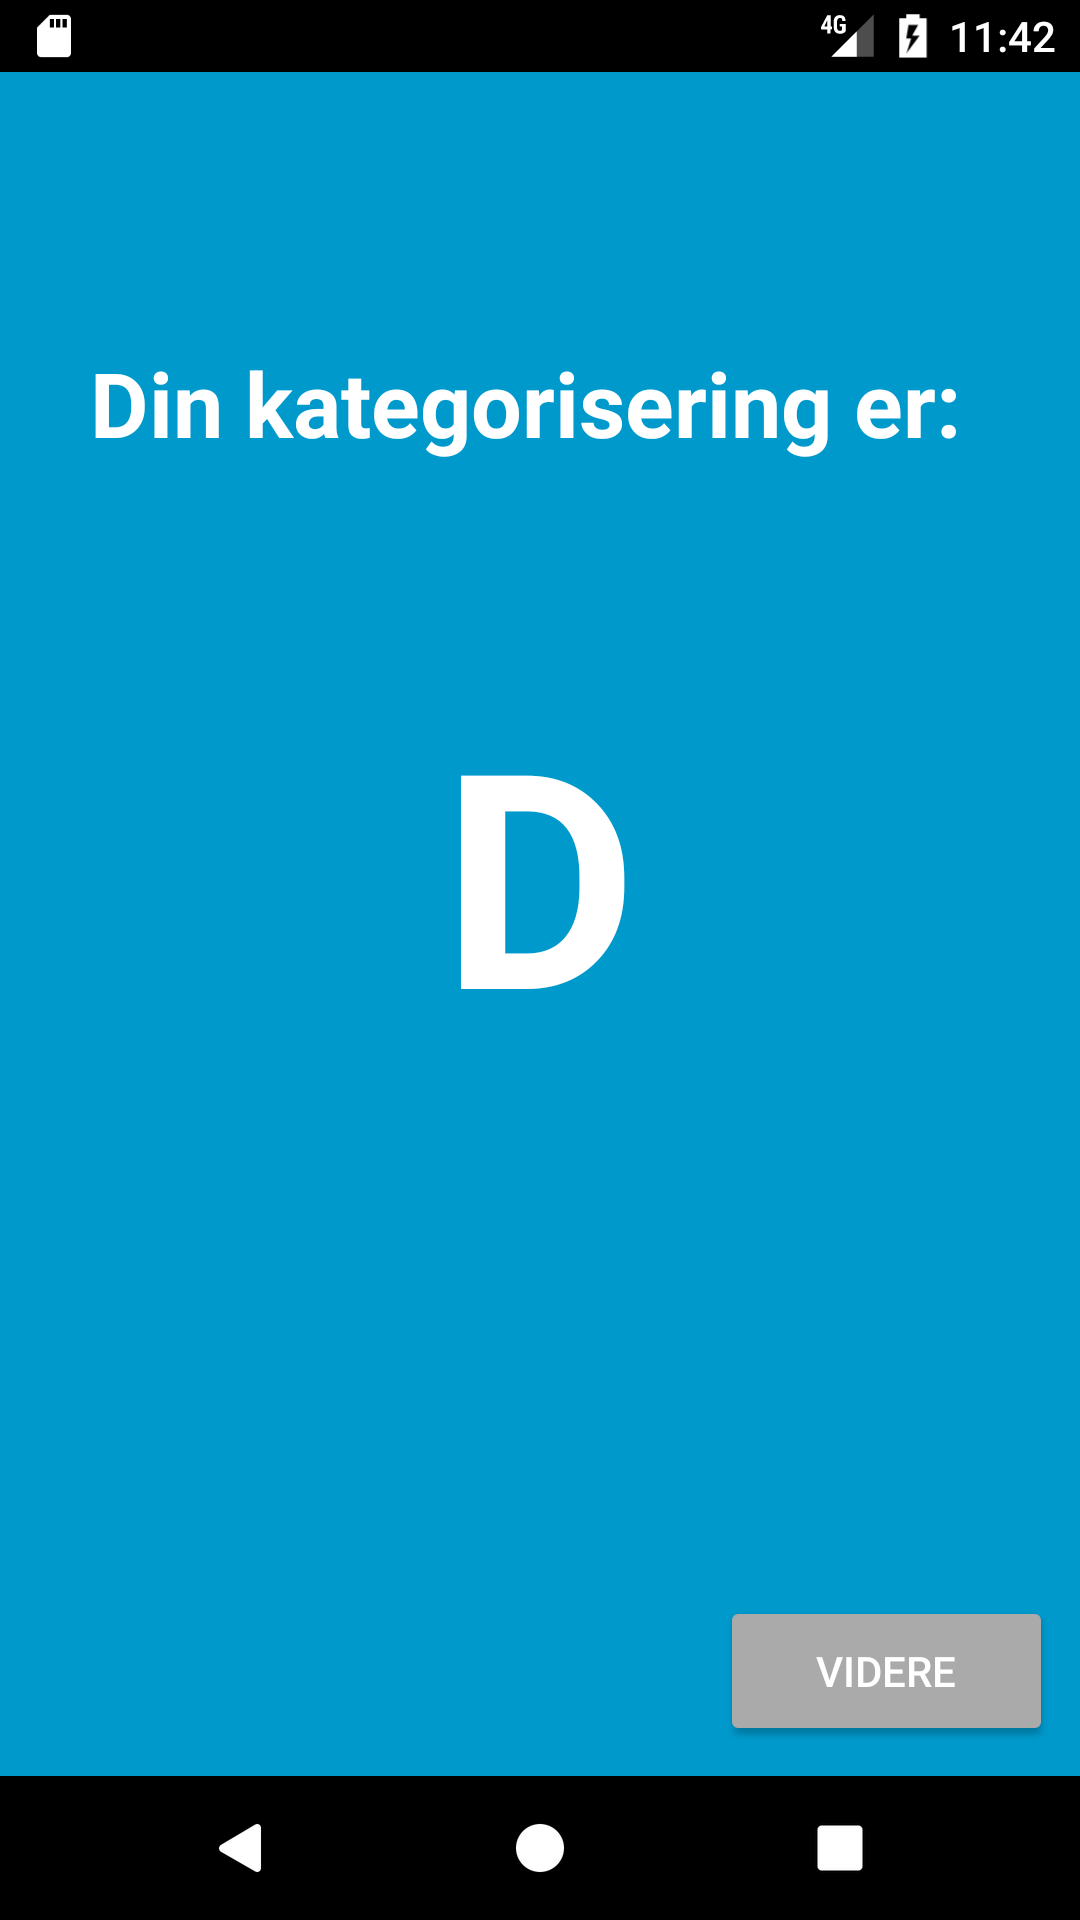
\includegraphics[width=0.20\textwidth, height=60mm]{figures/test/testkat3}} 
    \vspace{3mm}
               ~~~~~~~~\textbf{\textit{Figur 4}}~~~~~~~~~~~~~~\textbf{\textit{Figur 5}}~~~~~~~~~~~~~~\textbf{\textit{Figur 6}}~~~~~~~~~~~~~~~\textbf{\textit{Figur 7}}
    \newline
Resultater for test af kategorisering fremgår af ovenstående figurer. Fra venstre mod højre ses, at henholdsvis første til fjerde main flow viser de forventede kategoriseringer.
 \begin{itemize}[label={\checkmark}]
\item På baggrund af denne test er kravet for kategorisering er opfyldt
\end{itemize} 
\\ \hline
   \caption{Test af kategorisering.}
    \label{tab:testKategorisering}
\end{longtable}

\section{Tilpasning af træningsniveau}
I tilpasning af træningsniveau skal brugeren oplyses et anbefalet træningsniveau, med henblik på at tage højde for daglige variationer, ved at anvende parametrene kategorisering, daglig helbredstilstand og eventuel tidligere evaluering. Følgende krav blev opstillet til tilpasningen af træningsnivauet:

\begin{itemize}
\item Brugere skal kunne angive deres daglige helbredstilstand
\\
\textit{Dette er nødvendigt for tage højde for daglige variationer og derved tilpasse træningen for den enkelte bruger}
\end{itemize}

\noindent
Da der blev afgrænset til konditionstræning er testen kun udført med konditionstræning. Derudover er testen opdelt i tilpasning af træningsniveau med og uden evaluering, da der ved første anvendelse ikke eksisterer en evaluering. Testen for tilpasning af træningsniveau uden evaluering fremgår af \autoref{tab:testTilpasningudenevaluering} og med evaluering af \autoref{tab:testTilpasningmedevaluering}.

  \begin{longtable}{ | l | p{13cm} |} \hline
    \textbf{Test:} & Tilpasning af træningsniveau uden evaluering \\ \hline
     \textbf{Formål:} & Formålet er, at brugeren skal kunne angive ønsket træningsform, træningstype samt daglig helbredstilstand, hvorefter systemet, på baggrund af dette samt brugerens kategorisering, anbefaler et træningsniveau. Dette gøres ved at angive samme træningsform, og vælge mellem de tre forskellige træningstyper og helbredstilsande. Brugeren er i kategoriseringen A.
 \\ \hline
 	\textbf{Main flow:} &
 	1.~Vælg \textit{TRÆNING}, \textit{KONDITIONSTRÆNING}, \textit{LØB}, \textit{MEGET DÅRLIGT} og tryk videre efter hver handling.
 	\begin{itemize}
 	\item Anbefaling af træningstid er 10 min (\textbf{\textit{Figur 4}})
 	\end{itemize}
 	 2~Vælg \textit{TRÆNING}, \textit{KONDITIONSTRÆNING}, \textit{GÅ}, \textit{MODERAT} og tryk videre efter hver handling.
 	\begin{itemize}
 	\item Anbefaling af træningstid er 30 min (\textbf{\textit{Figur 5}})
 	\end{itemize}	
3.~Vælg \textit{TRÆNING}, \textit{KONDITIONSTRÆNING}, \textit{CYKEL}, \textit{MEGET GODT} og tryk videre efter hver handling.
 \begin{itemize}
  \item Anbefaling af træningstid er 50 min (\textbf{\textit{Figur 6}})
  \end{itemize}
 \\  \hline
 \textbf{Resultat:} &\hspace{1.5mm}
  \raisebox{-\totalheight}{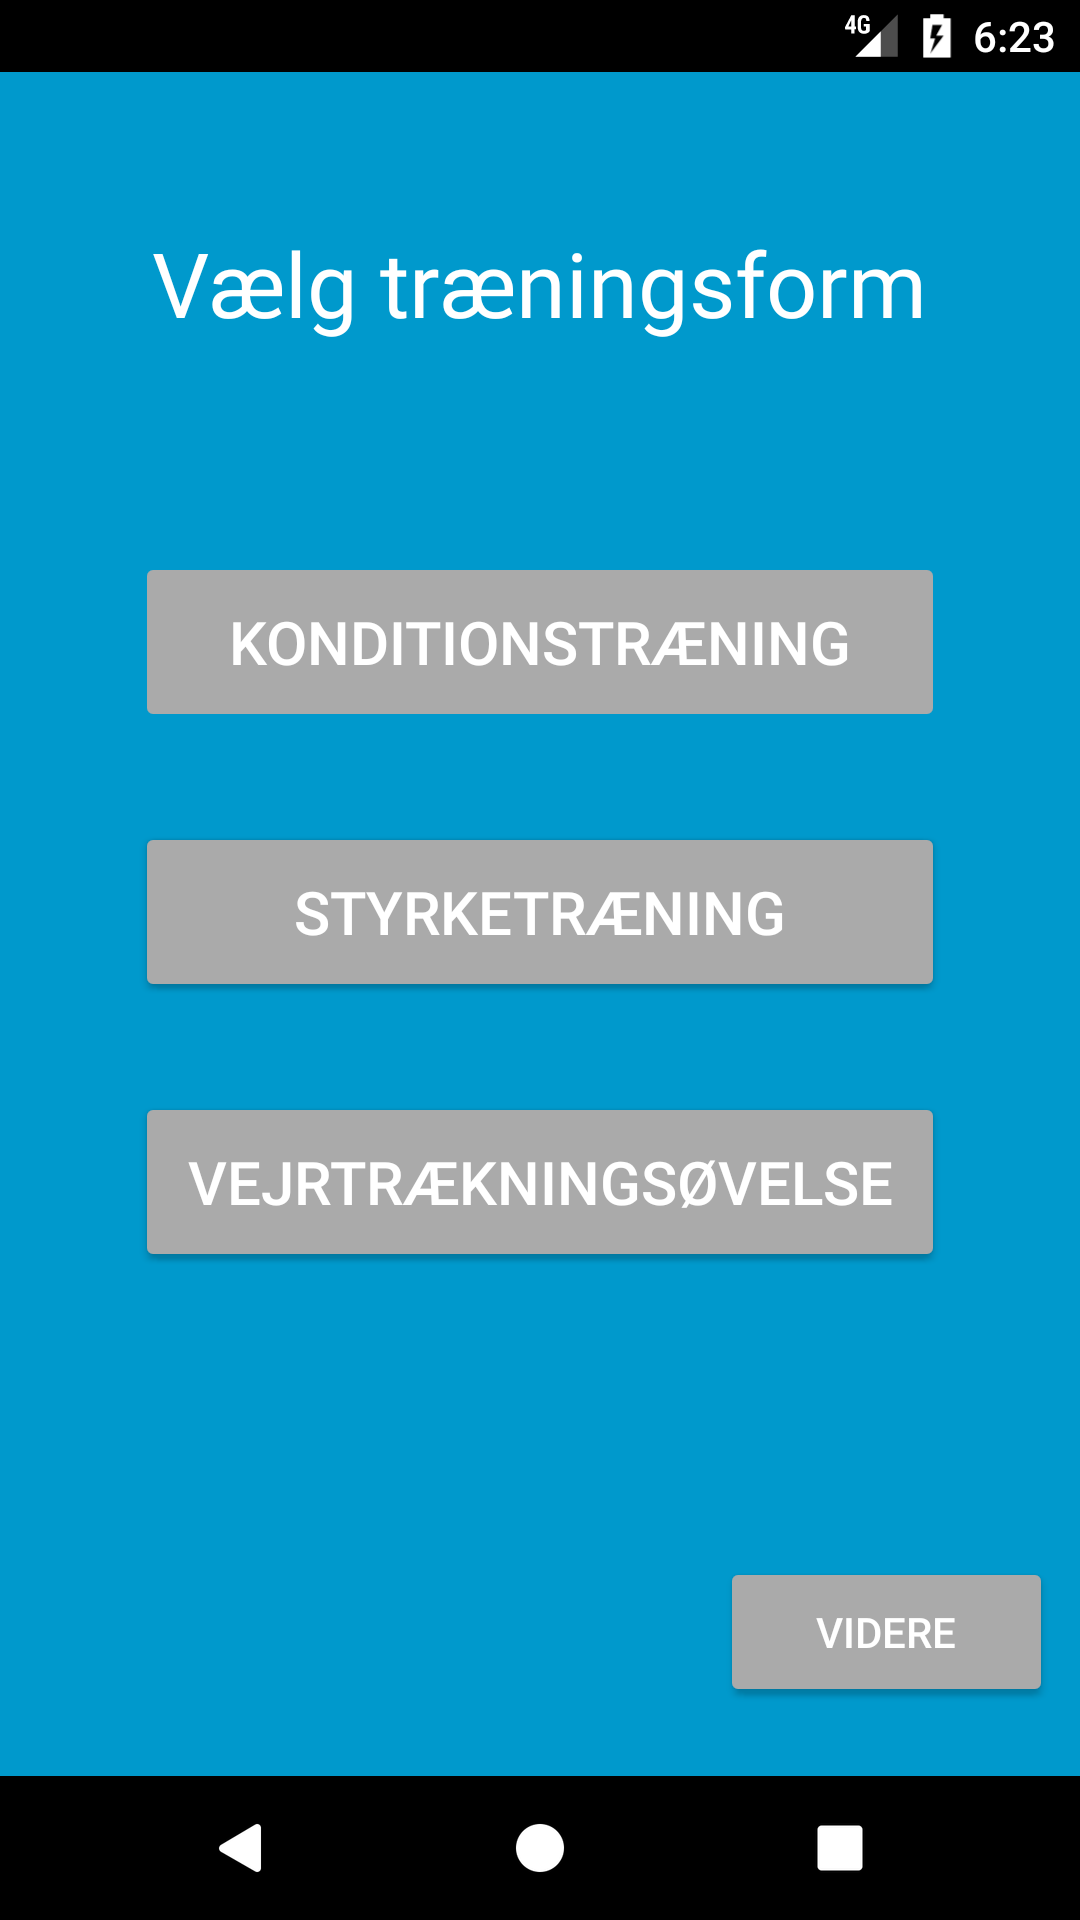
\includegraphics[width=0.24\textwidth, height=60mm]{figures/test/tilpasningny}} 
  \hspace{5mm}
   \raisebox{-\totalheight}{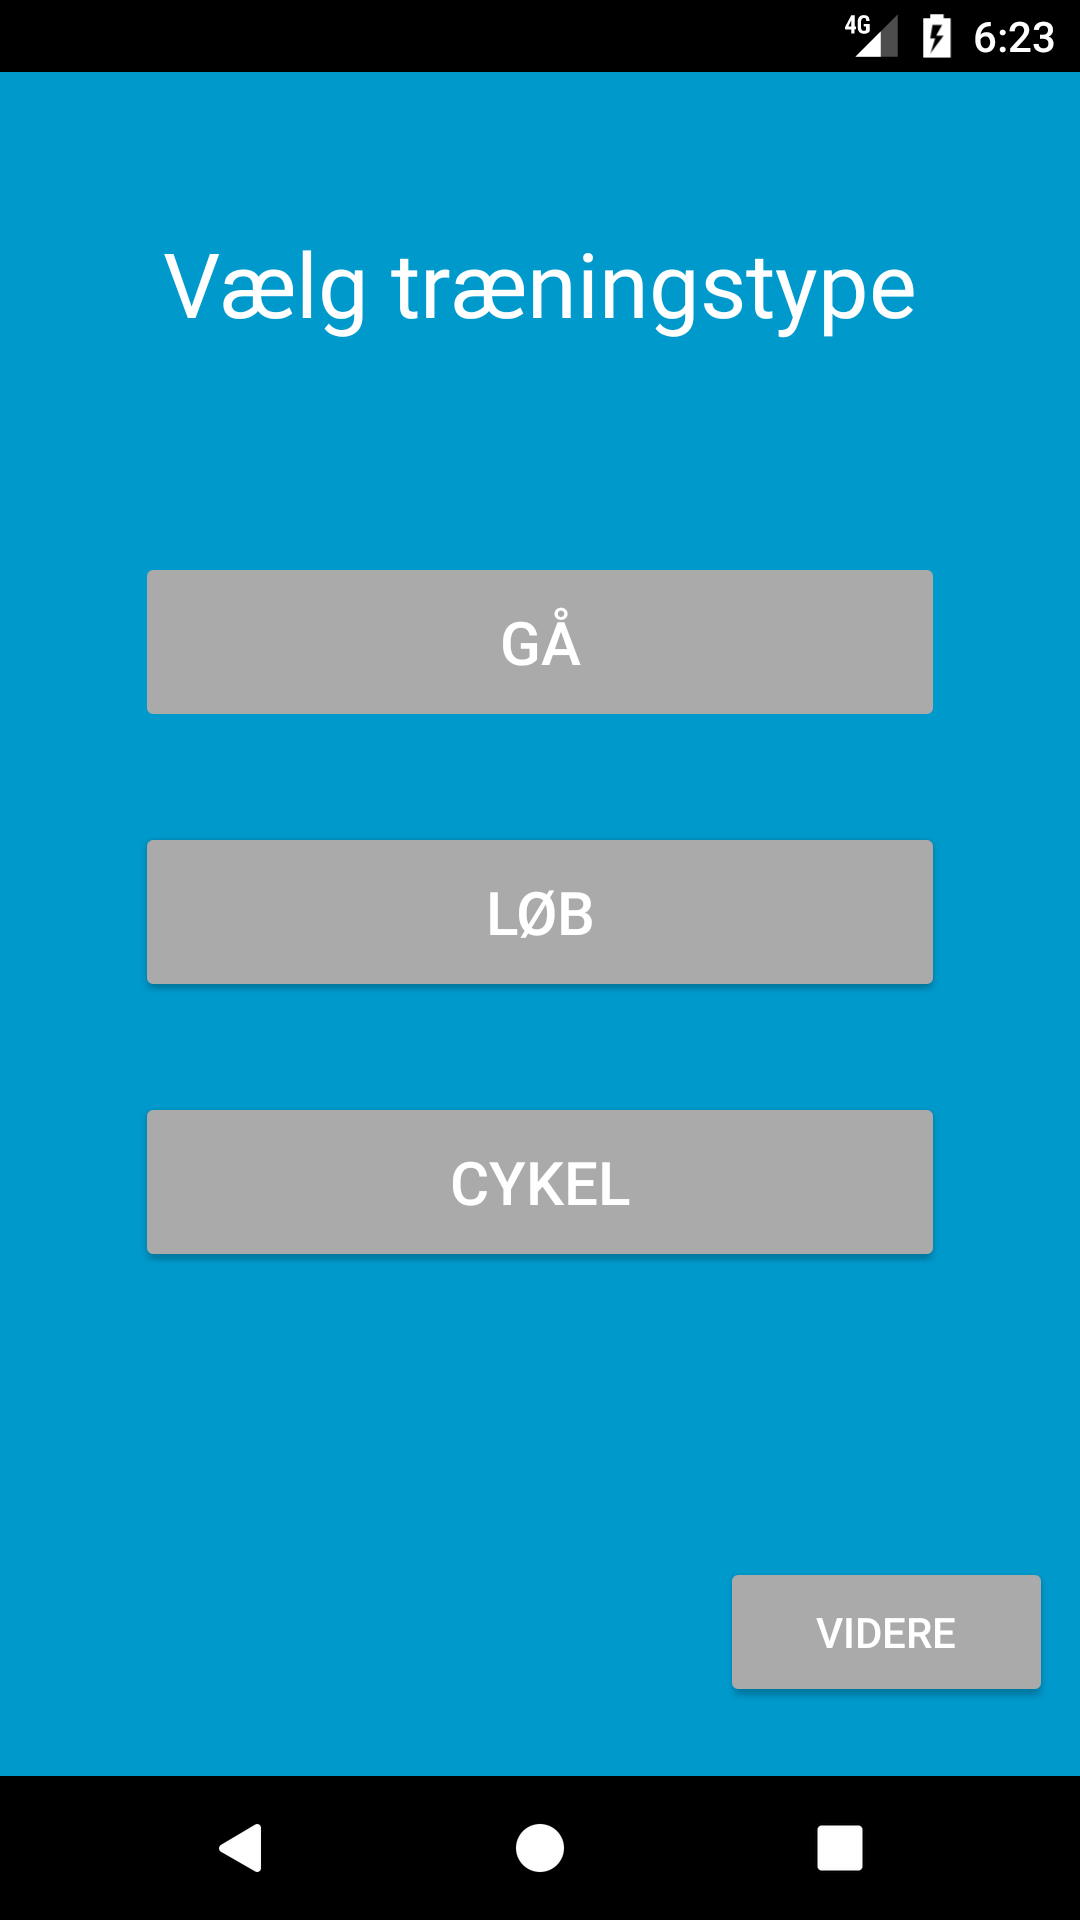
\includegraphics[width=0.24\textwidth, height=60mm]{figures/test/tilpasningny1}} 
  \hspace{5mm}
   \raisebox{-\totalheight}{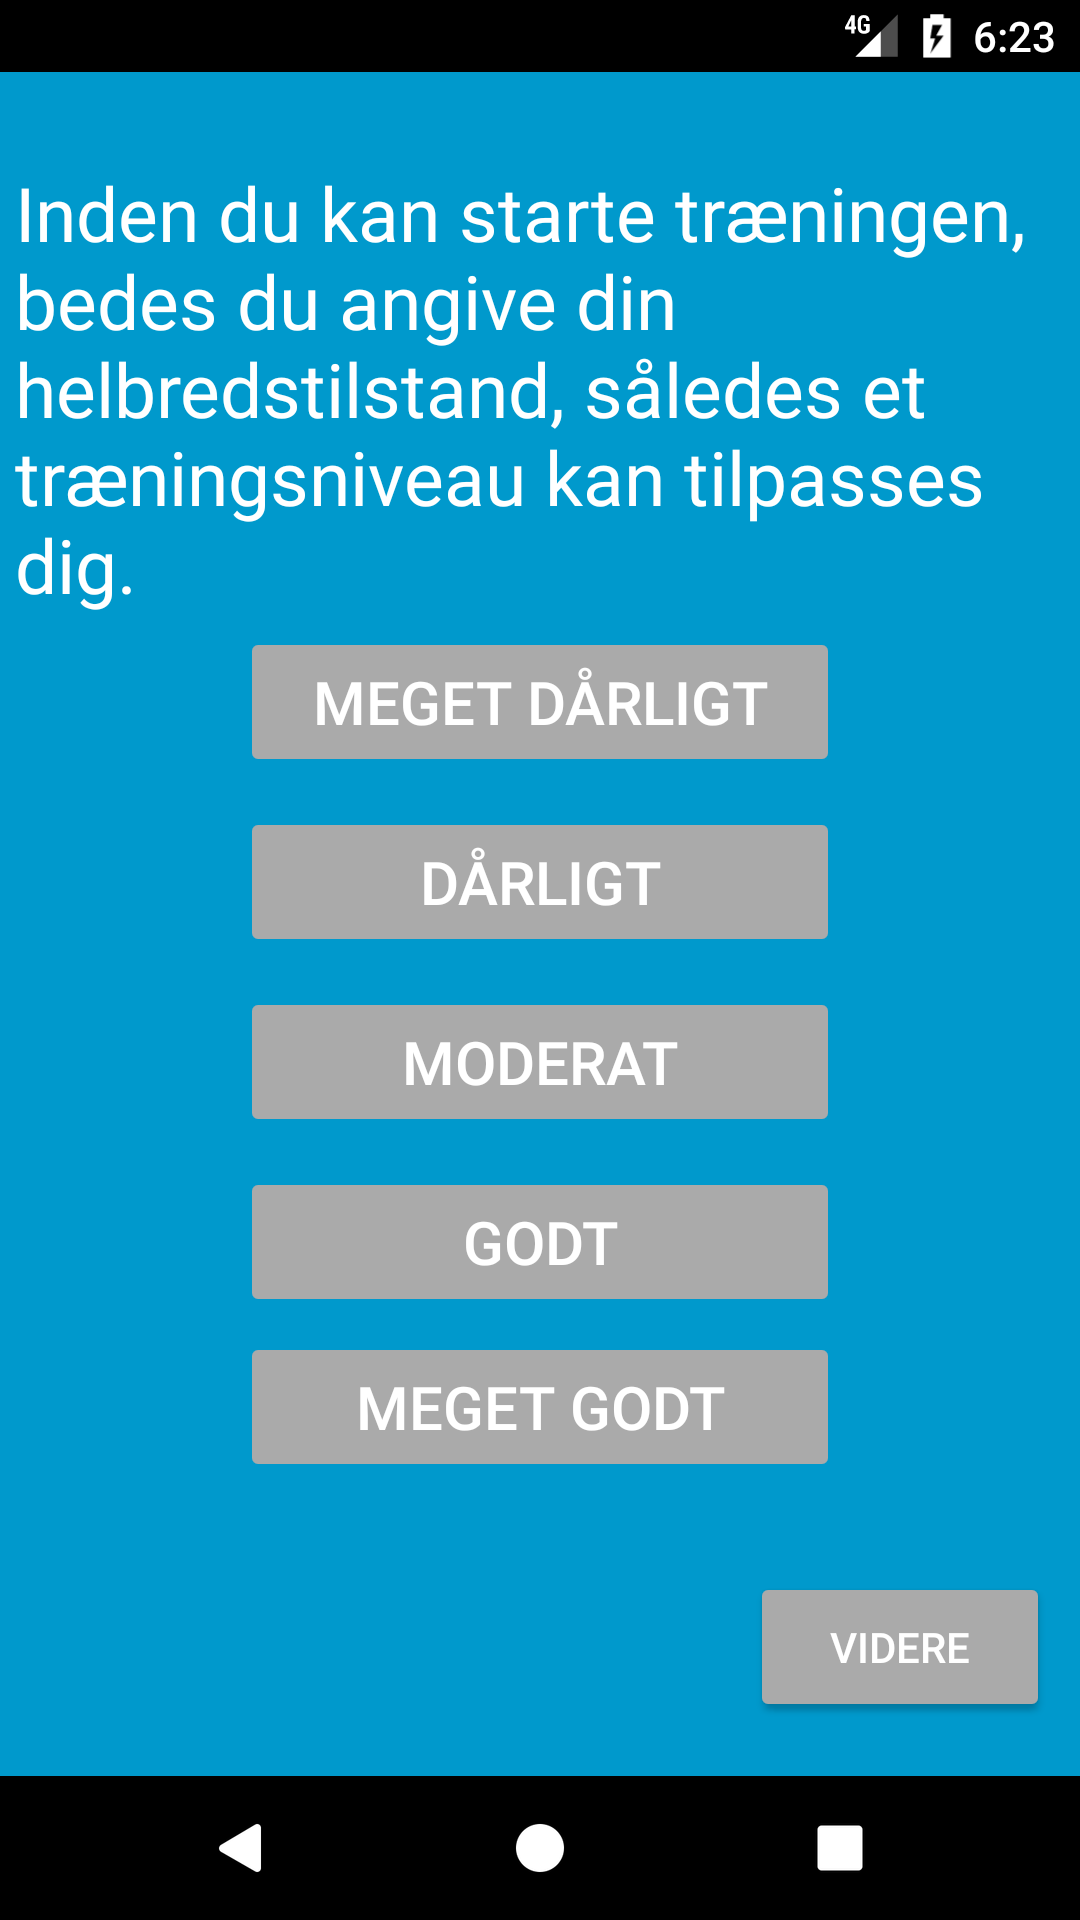
\includegraphics[width=0.24\textwidth, height=60mm]{figures/test/tilpasningny2}} 
\vspace{3mm}
        ~~~~~~~~~~~ \textbf{\textit{Figur 1}}~~~~~~~~~~~~~~~~~~~~~~~~\textbf{\textit{Figur 2}}~~~~~~~~~~~~~~~~~~~~~~~~\textbf{\textit{Figur 3}}
    \newline
Ovenstående figurer viser grænsefladerne for valg af træningsform, træningstype og daglig helbredstilstand. Disse grænseflader vises før grænsefladen for anbefalet træningstid. 
   \\ \hline
  \textbf{} &\hspace{1.5mm}
  \raisebox{-\totalheight}{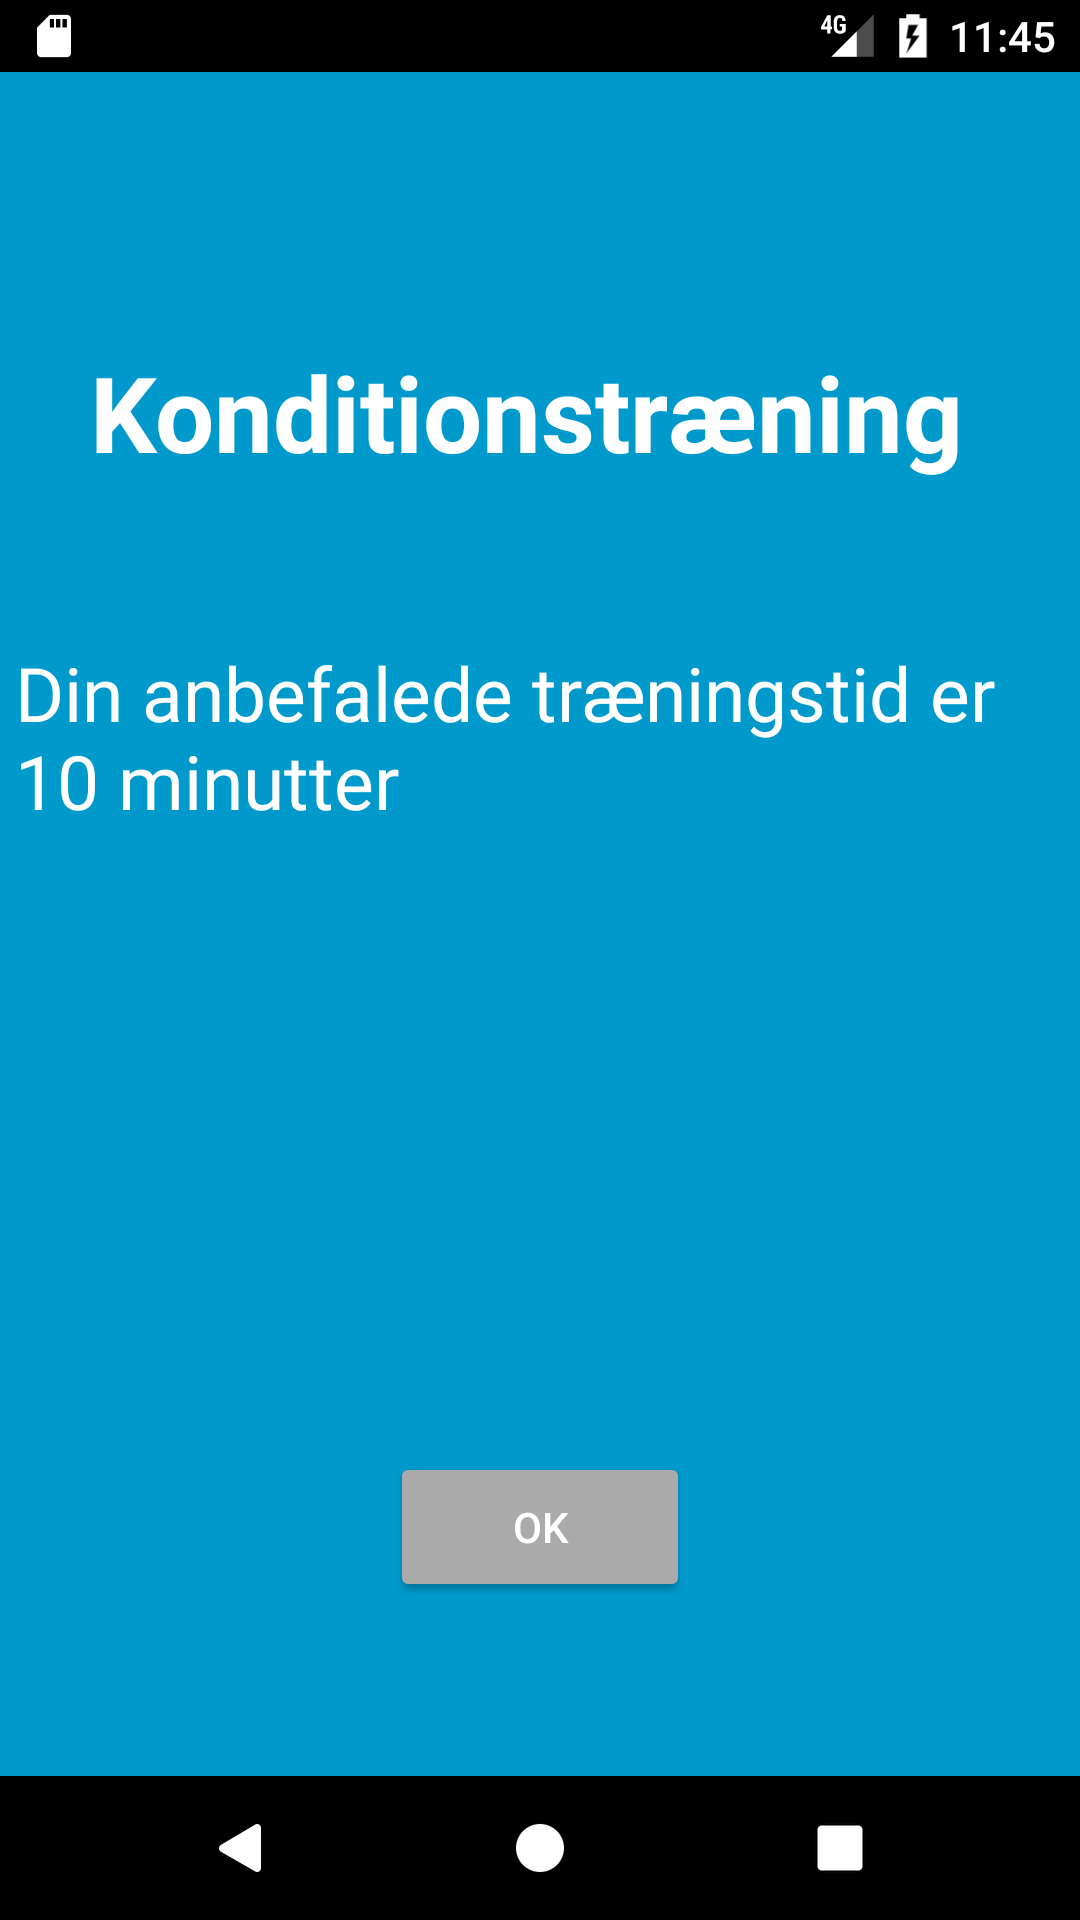
\includegraphics[width=0.24\textwidth, height=60mm]{figures/test/tilpasning1}} 
  \hspace{5mm}
   \raisebox{-\totalheight}{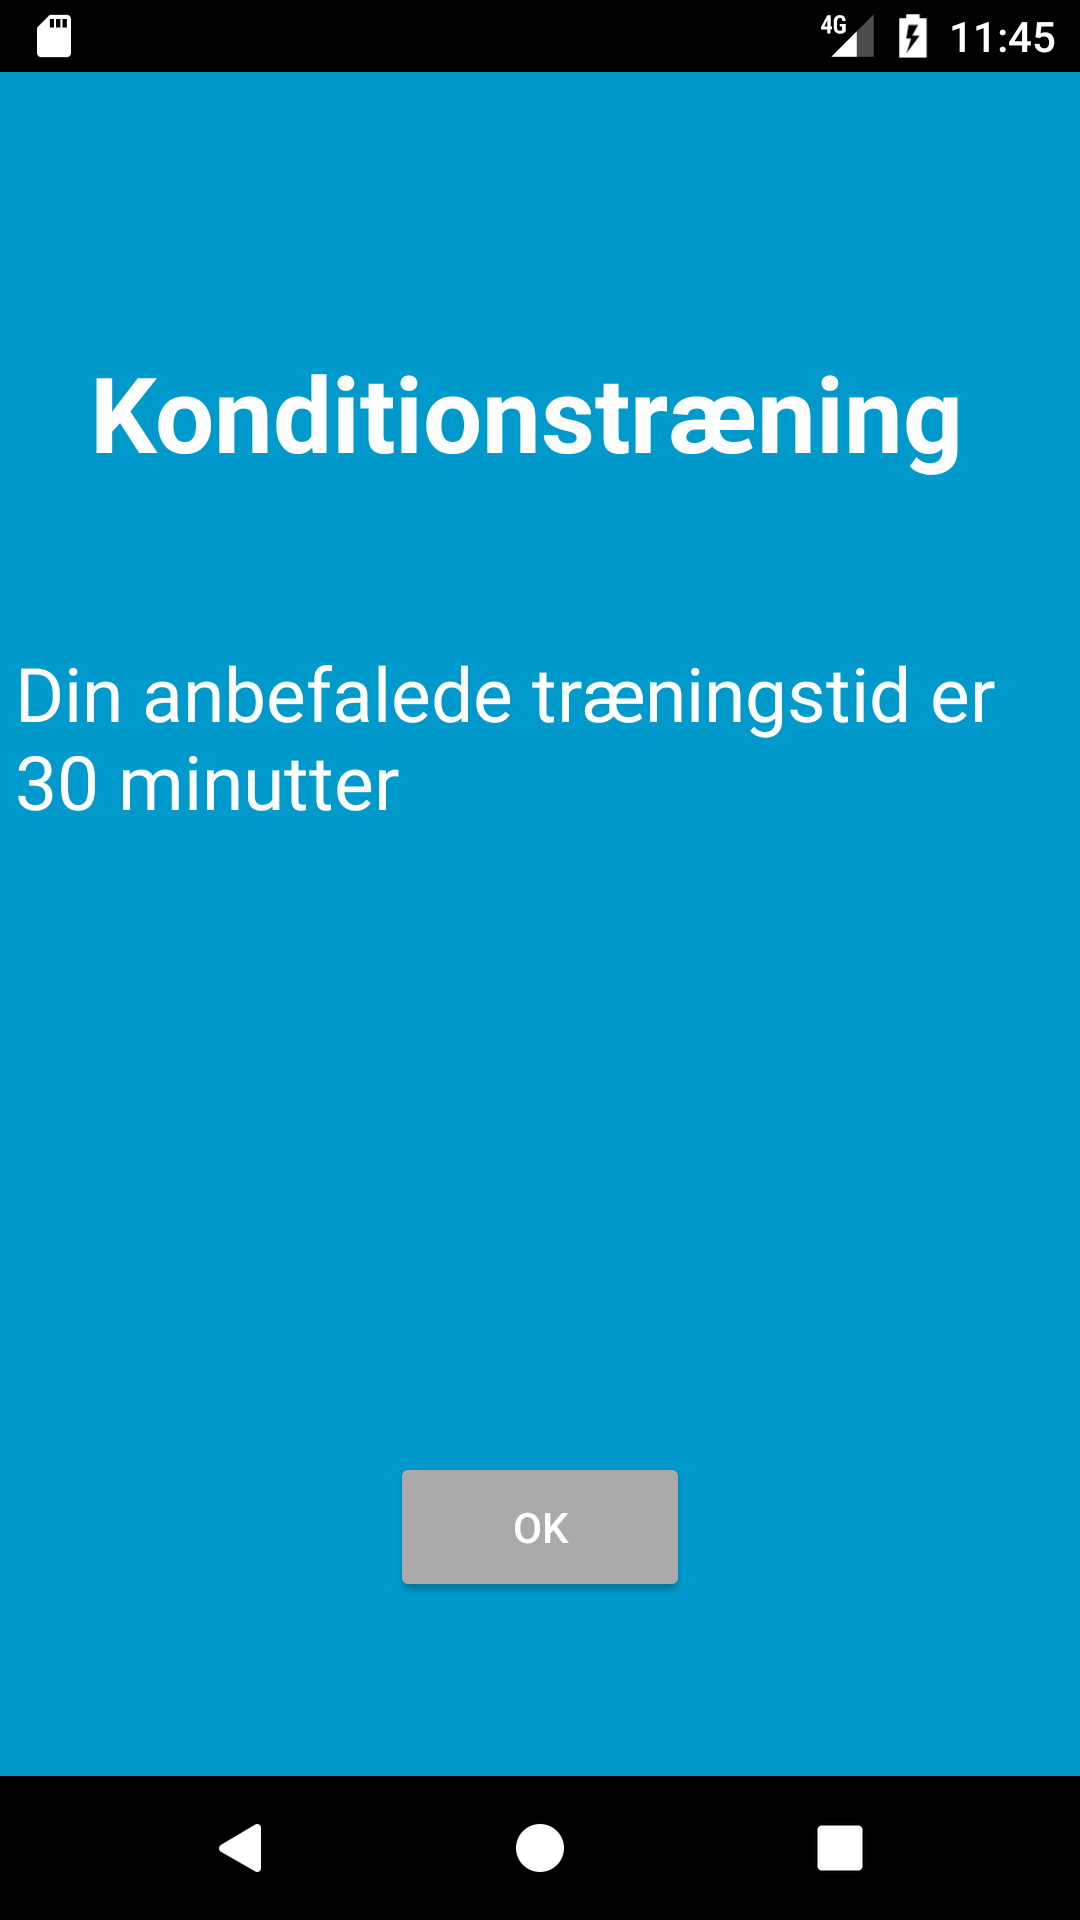
\includegraphics[width=0.24\textwidth, height=60mm]{figures/test/tilpasning}} 
     \hspace{5mm}
    \raisebox{-\totalheight}{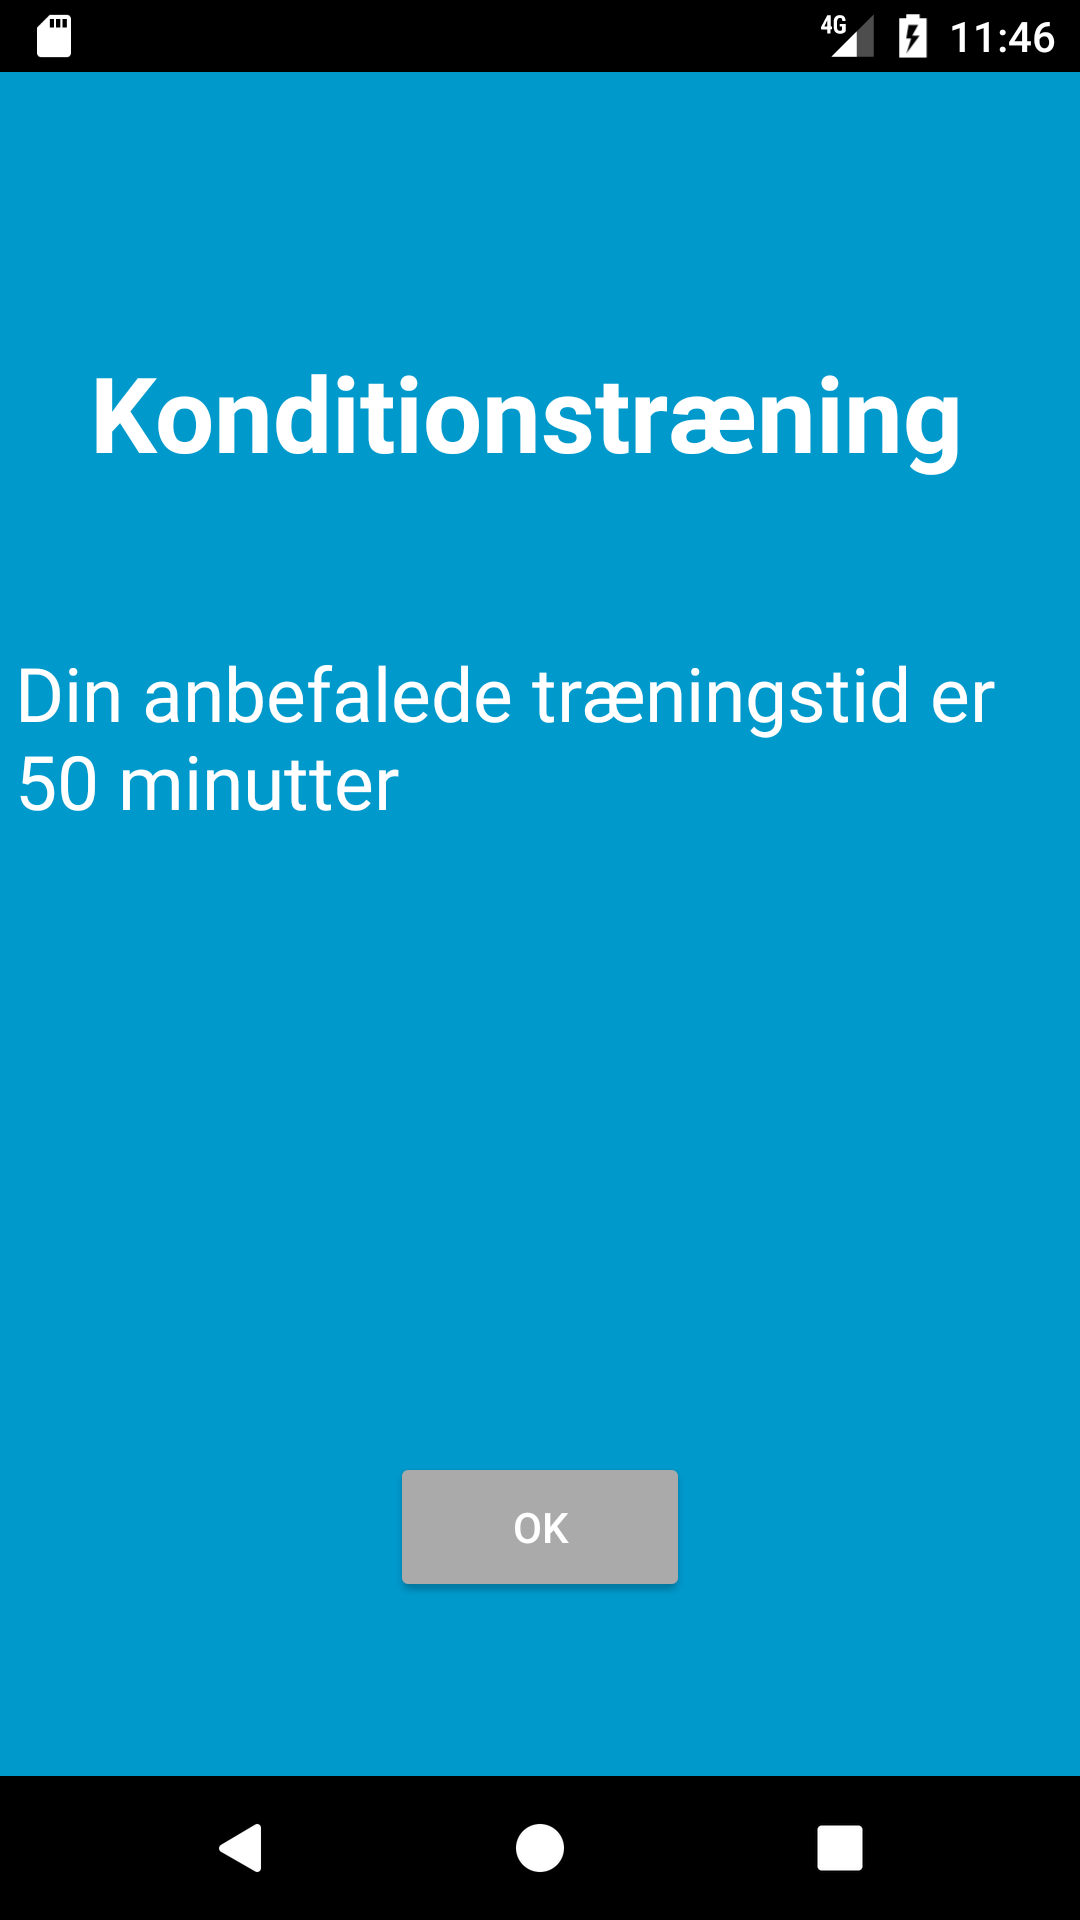
\includegraphics[width=0.24\textwidth, height=60mm]{figures/test/tilpasning2}} 
    \vspace{3mm}
        ~~~~~~~~~~~ \textbf{\textit{Figur 4}}~~~~~~~~~~~~~~~~~~~~~~~~\textbf{\textit{Figur 5}}~~~~~~~~~~~~~~~~~~~~~~~~\textbf{\textit{Figur 6}}
    \newline
    Resultater for test af tilpasning af træningsniveau uden evaluering fremgår af ovenstående figurer. Fra venstre mod højre ses, at henholdsvis første til tredje main flow viser de forventede anbefalinger af træningstider. 
 \\ \hline
   \caption{Test af tilpasning af træningsniveau uden evaluering.}
    \label{tab:testTilpasningudenevaluering}
\end{longtable}


  \begin{longtable}{ | l | p{13cm} |} \hline
    \textbf{Test:} & Tilpasning af træningsniveau med evaluering \\ \hline
     \textbf{Formål:} & Formålet er, at brugeren skal kunne angive ønsket træningsform, træningstype samt daglig helbredstilstand, hvorefter systemet på baggrund af dette samt kategorisering og tidligere evaluering skal anbefale et træningsniveau. Dette gøres ved at angive samme træningsform, og vælge mellem de tre forskellige træningstyper og helbredstilstande. Brugeren er i kategoriseringen A og har forinden træningen angivet evaluering for samme træning samt helbredstilstand.
 \\ \hline
 	\textbf{Main flow:} &
 	1.~Tidligere evaluering af samme træning er :-D og helbredstilstand meget dårligt. Vælg \textit{TRÆNING}, \textit{KONDITIONSTRÆNING}, \textit{LØB}, \textit{MEGET DÅRLIGT} og tryk videre efter hver handling.
 	\begin{itemize}
 	\item Anbefaling af træningstid er 15 min (\textbf{\textit{Figur 1}})
 	\end{itemize} 	
 	 2.~Tidligere evaluering af samme træning er :-) og helbredstilstand moderat. Vælg \textit{TRÆNING}, \textit{KONDITIONSTRÆNING}, \textit{GÅ}, \textit{MODERAT} og tryk videre efter hver handling.
 	\begin{itemize}
 	\item Anbefaling af træningstid er 30 min (\textbf{\textit{Figur 2}})
 	\end{itemize}	
3.~Tidligere evaluering af samme træning er :-( og helbredstilstand meget godt. Vælg \textit{TRÆNING}, \textit{KONDITIONSTRÆNING}, \textit{CYKEL}, \textit{MEGET GODT} og tryk videre efter hver handling.
 \begin{itemize}
  \item Anbefaling af træningstid er 45 min (\textbf{\textit{Figur 3}})
  \end{itemize}
 \\  \hline
 \textbf{Resultat:} &\hspace{1.5mm}
  \raisebox{-\totalheight}{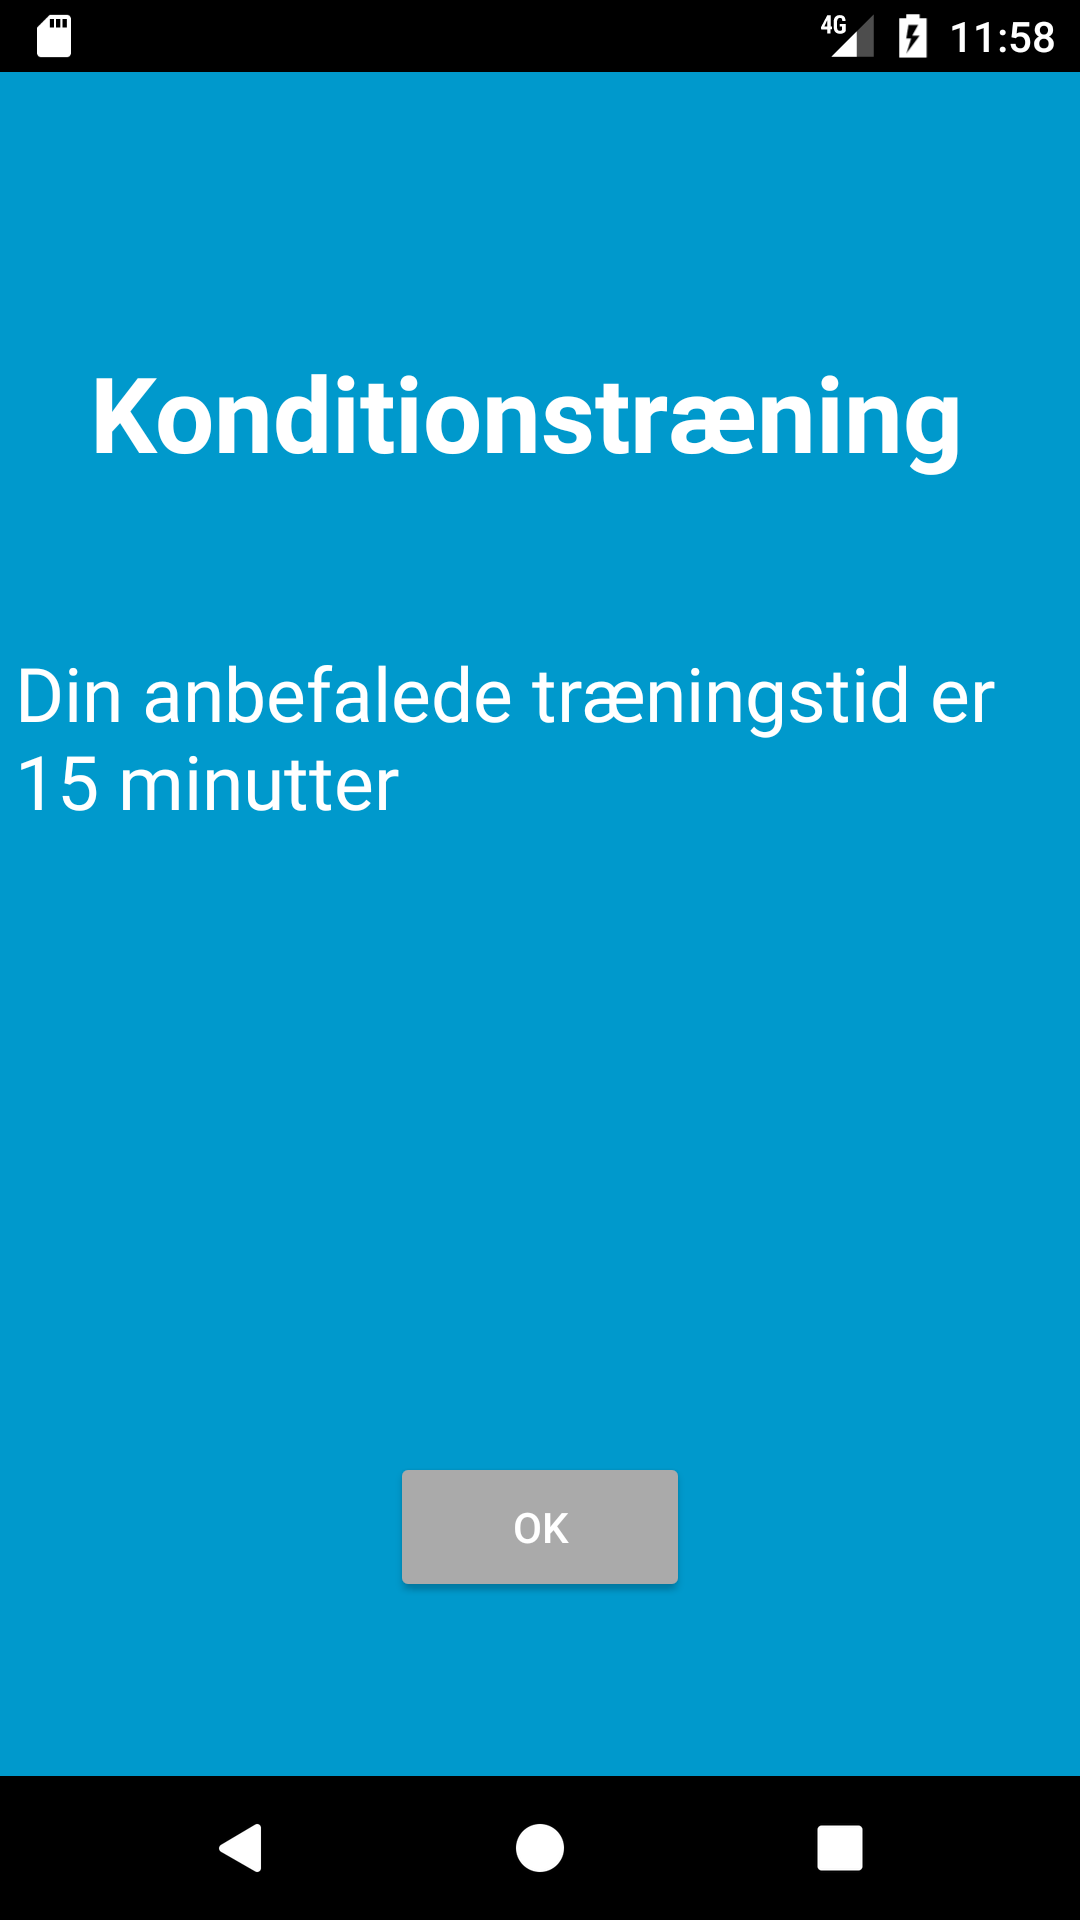
\includegraphics[width=0.24\textwidth, height=60mm]{figures/test/tilpasning4}} 
  \hspace{5mm}
   \raisebox{-\totalheight}{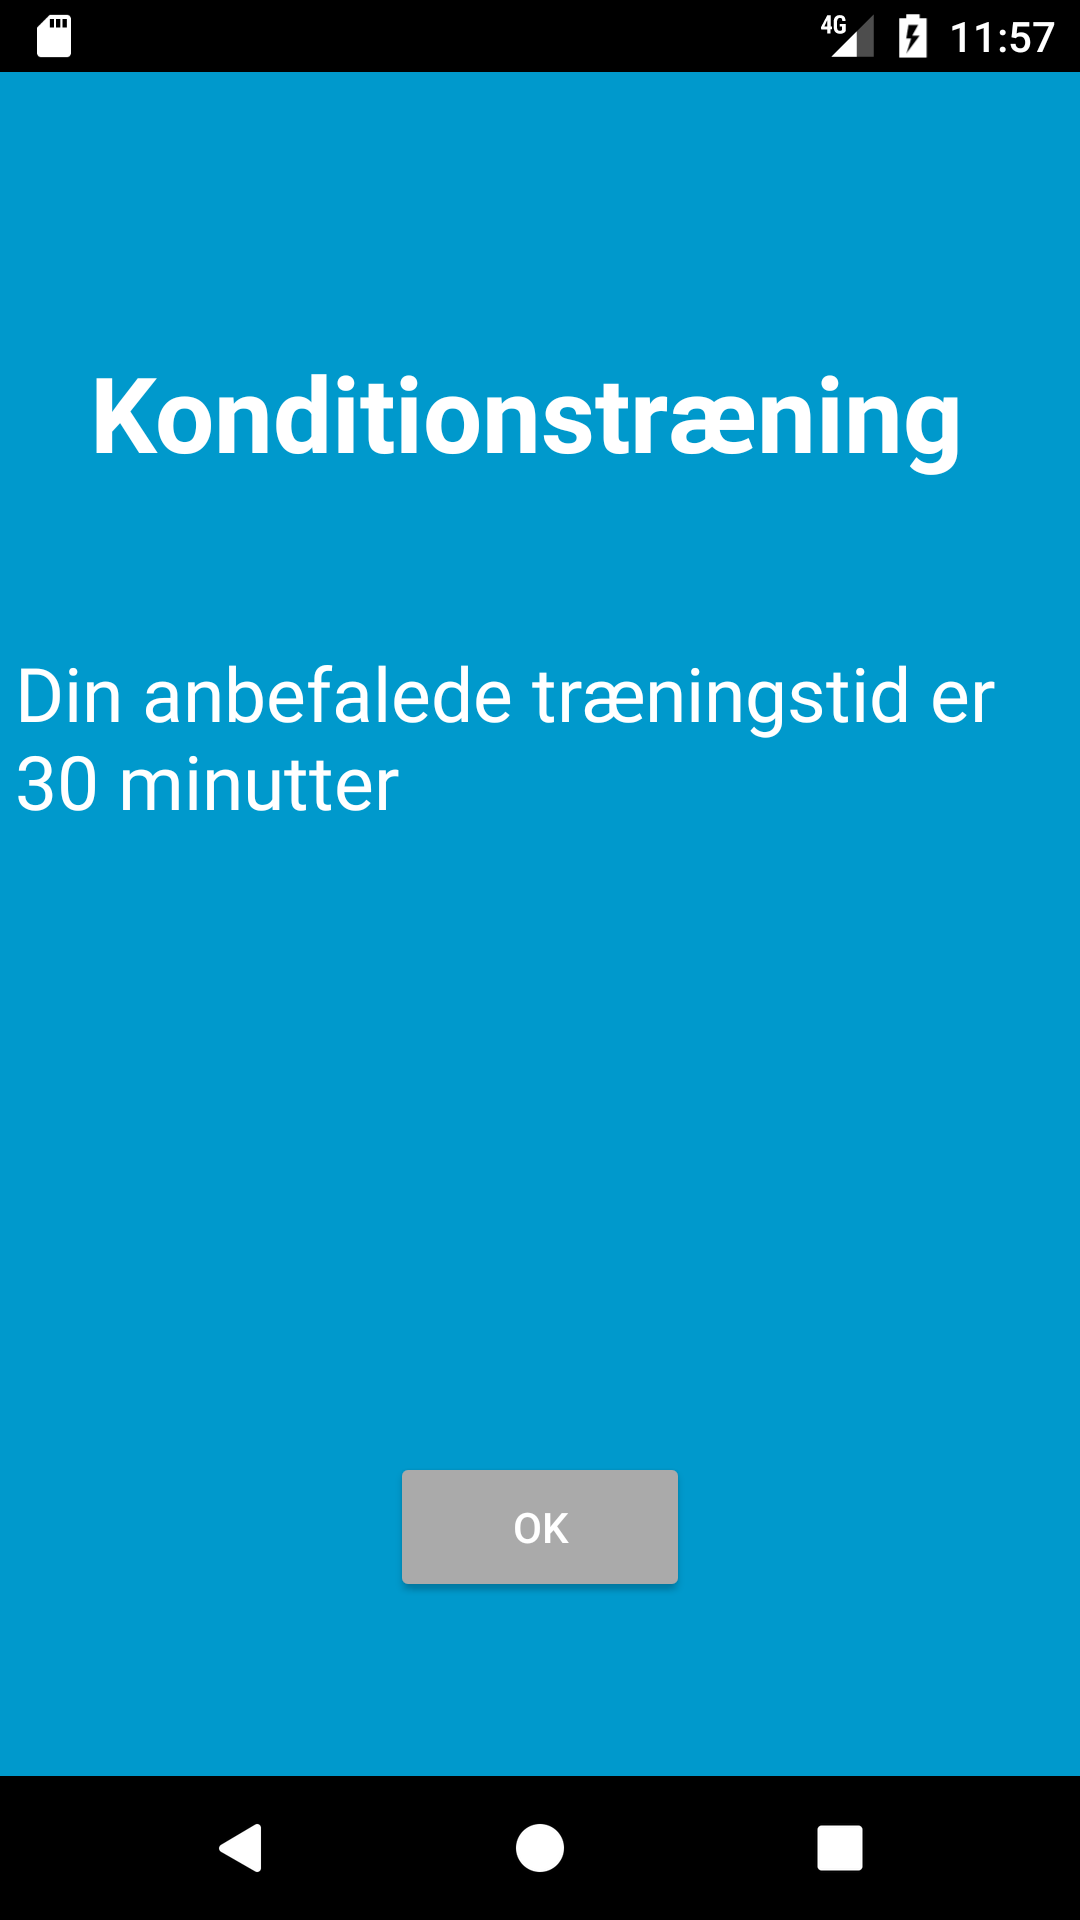
\includegraphics[width=0.24\textwidth, height=60mm]{figures/test/tilpasning3}} 
     \hspace{5mm}
    \raisebox{-\totalheight}{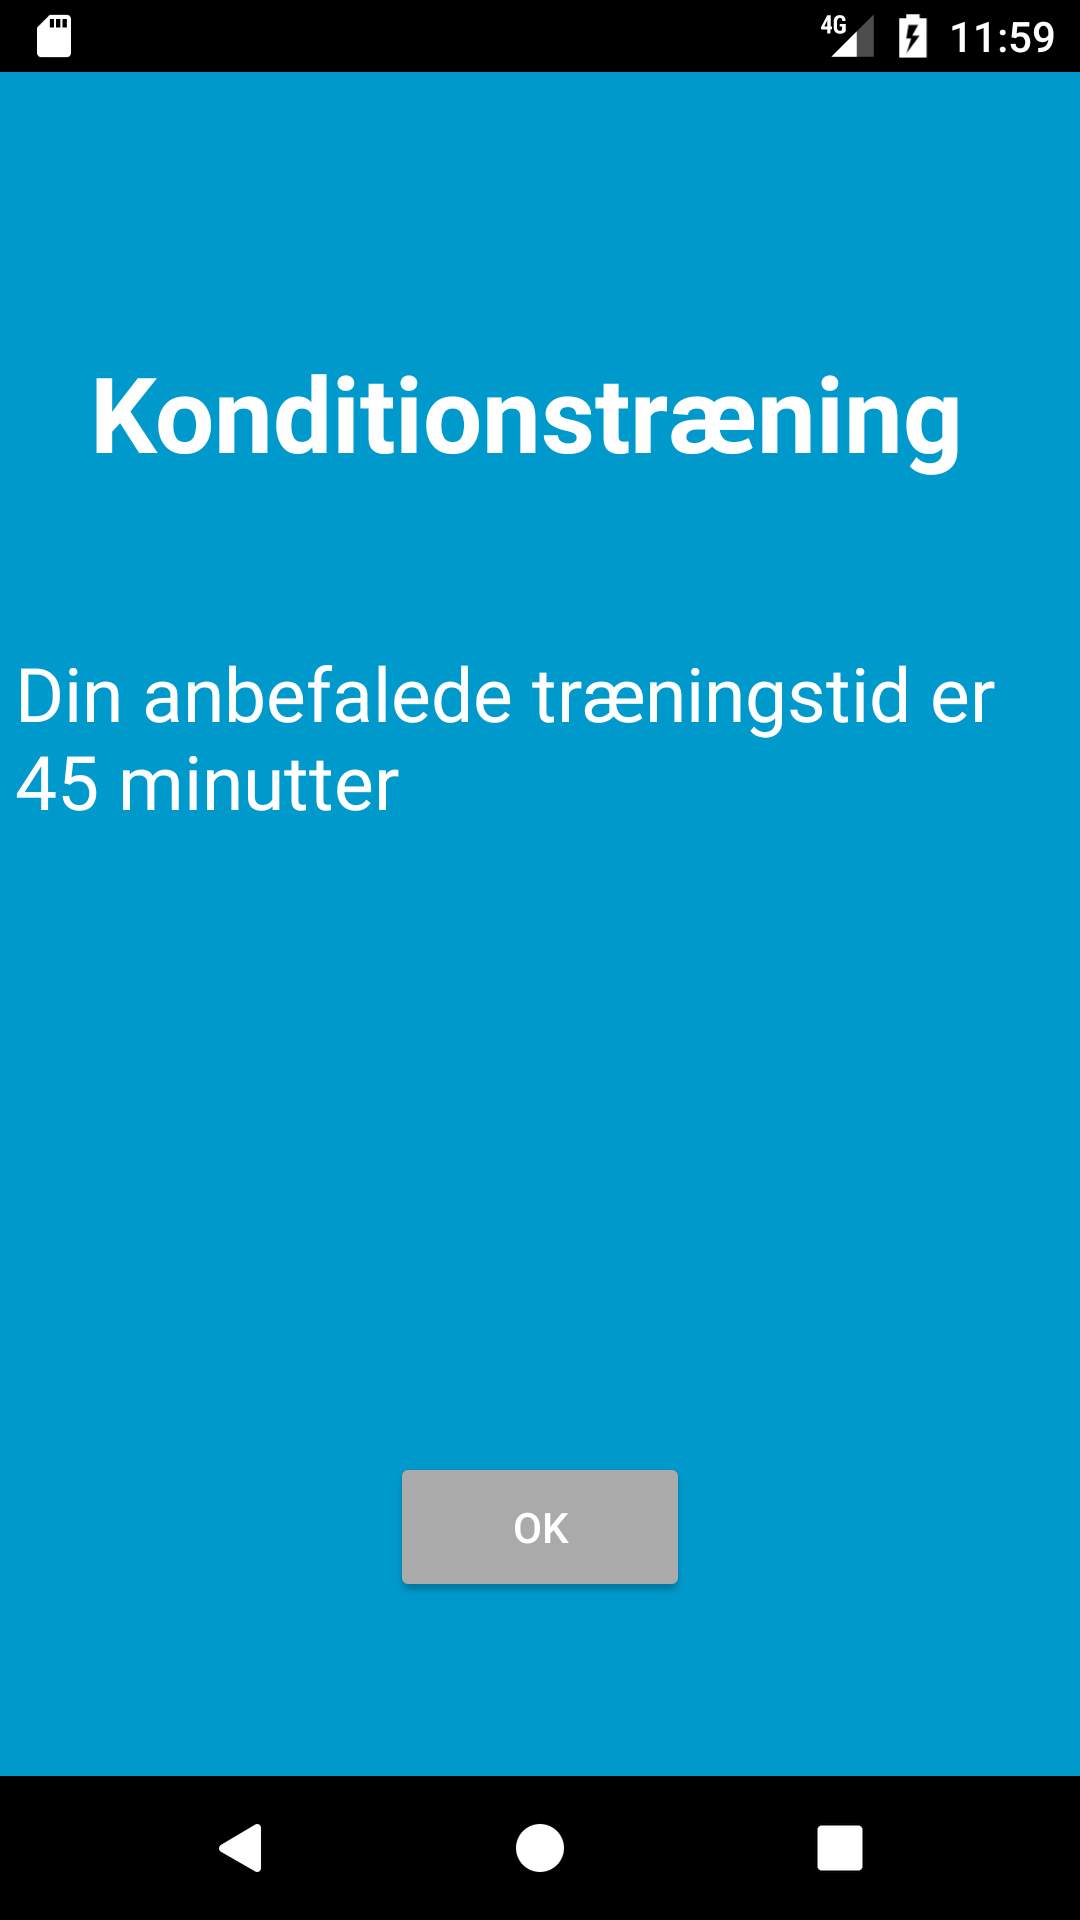
\includegraphics[width=0.24\textwidth, height=60mm]{figures/test/tilpasning5}} 
    \vspace{3mm}
        ~~~~~~~~~~~ \textbf{\textit{Figur 1}}~~~~~~~~~~~~~~~~~~~~~~~~\textbf{\textit{Figur 2}}~~~~~~~~~~~~~~~~~~~~~~~~\textbf{\textit{Figur 3}}
    \newline
 Resultater for test af tilpasning af træningsniveau med evaluering fremgår af ovenstående figurer. Fra venstre mod højre ses, at henholdsvis første til tredje main flow viser de forventede anbefalinger af træningstider. 
 \begin{itemize}[label={\checkmark}]
\item På baggrund af test af tilpasning af træningsniveau uden og med evaluering er kravet for tilpasning af træningsniveau opfyldt 
\end{itemize}
    \\ \hline
   \caption{Test af tilpasning af træningsniveau med evaluering.}
    \label{tab:testTilpasningmedevaluering}
\end{longtable}


\section{Træning}
Systemet skal muliggøre måling af tid og afstand under træning, derudover skal brugeren have mulighed for at evaluere træningen efterfølgende. For træning er følgende krav opstillet:

\begin{itemize}
\item Systemet skal kunne måle tid via timer og afstand via GPS
\\
\textit{Dette er nødvendigt for at monitorere træningen}
\item Brugere skal kunne evaluere hver træning
\\
\textit{Dette er nødvendigt for at tilpasse træningen yderligere efter den enkelte bruger}
\item Systemet skal kunne sende en daglig notifikation for således at påminde brugeren om træning
\\
\textit{Dette er nødvendigt for at kunne motivere brugere til at udføre træning}
\end{itemize}

\noindent
For at teste, hvorvidt de opstillede krav til træningen er opfyldt, udføres testen, som fremgår af \autoref{tab:testTraening}.

%\begin{table} [H]
%	\centering
  \begin{longtable}{ | p{2cm} | p{13cm} |} \hline
    \textbf{Test:} & Træning \\ \hline
  \textbf{Formål:} & Formålet er, at systemet skal kunne måle tid og afstand under træningen. Når brugeren har afsluttet træning, skal måleenhederne stoppe, og brugeren skal kunne angive evaluering. Dette gøres ved at måle tid og afstand samt evaluere træningen efterfølgende. Derudover skal en notifikation forekomme dagligt.
 \\ \hline
 	\textbf{Main flow:} & 1.~Tryk \textit{START TRÆNING} og lad træningen forløbe i minimum 2 minutter. Tryk herefter \textit{STOP TRÆNING}.
 	\begin{itemize}
 	\item Tiden er over 2 minutter (\textbf{\textit{Figur 2}})
 	\end{itemize}	
 	2.~Tryk \textit{START TRÆNING} åben Extended controls, som fremgår af \autoref{fig:emulatorExtend}. Sæt herefter longitude samt latitude til 0 og tryk send. Ændre begge til 0.01 og tryk send. Ændre derefter begge til 0.02 og tryk send. Tryk herefter \textit{STOP TRÆNING}. De forventede afstande er beregnet ved \autoref{equ:GPS}. 
 	\begin{itemize}
 	\item Afstand ved 0 er 0 km (\textbf{\textit{Figur 4}})
 	\item Afstand ved 0.01 er 1.57 km (\textbf{\textit{Figur 5}})
 	\item Afstand ved 0.02 er 3.14 km (\textbf{\textit{Figur 6}})
	\end{itemize}
  3.~Tryk \textit{START TRÆNING} og tryk herefter \textit{STOP TRÆNING} og 	bekræft. Angiv herefter \textit{:-)} og tryk videre.
  \begin{itemize}
  \item Evaluering er gemt i databasen (\textbf{\textit{Figur 9}})
  \end{itemize}
   4.~Vent til klokken 15 med at udføre en træning 
  \begin{itemize}
  \item Notifikation starter klokken 15 (\textbf{\textit{Figur 11 og 12}})
  \vspace{1mm}
  \end{itemize}
\\ \hline
\textbf{Resultat main flow 1:} &\hspace{1.5mm}
    \raisebox{-\totalheight}    {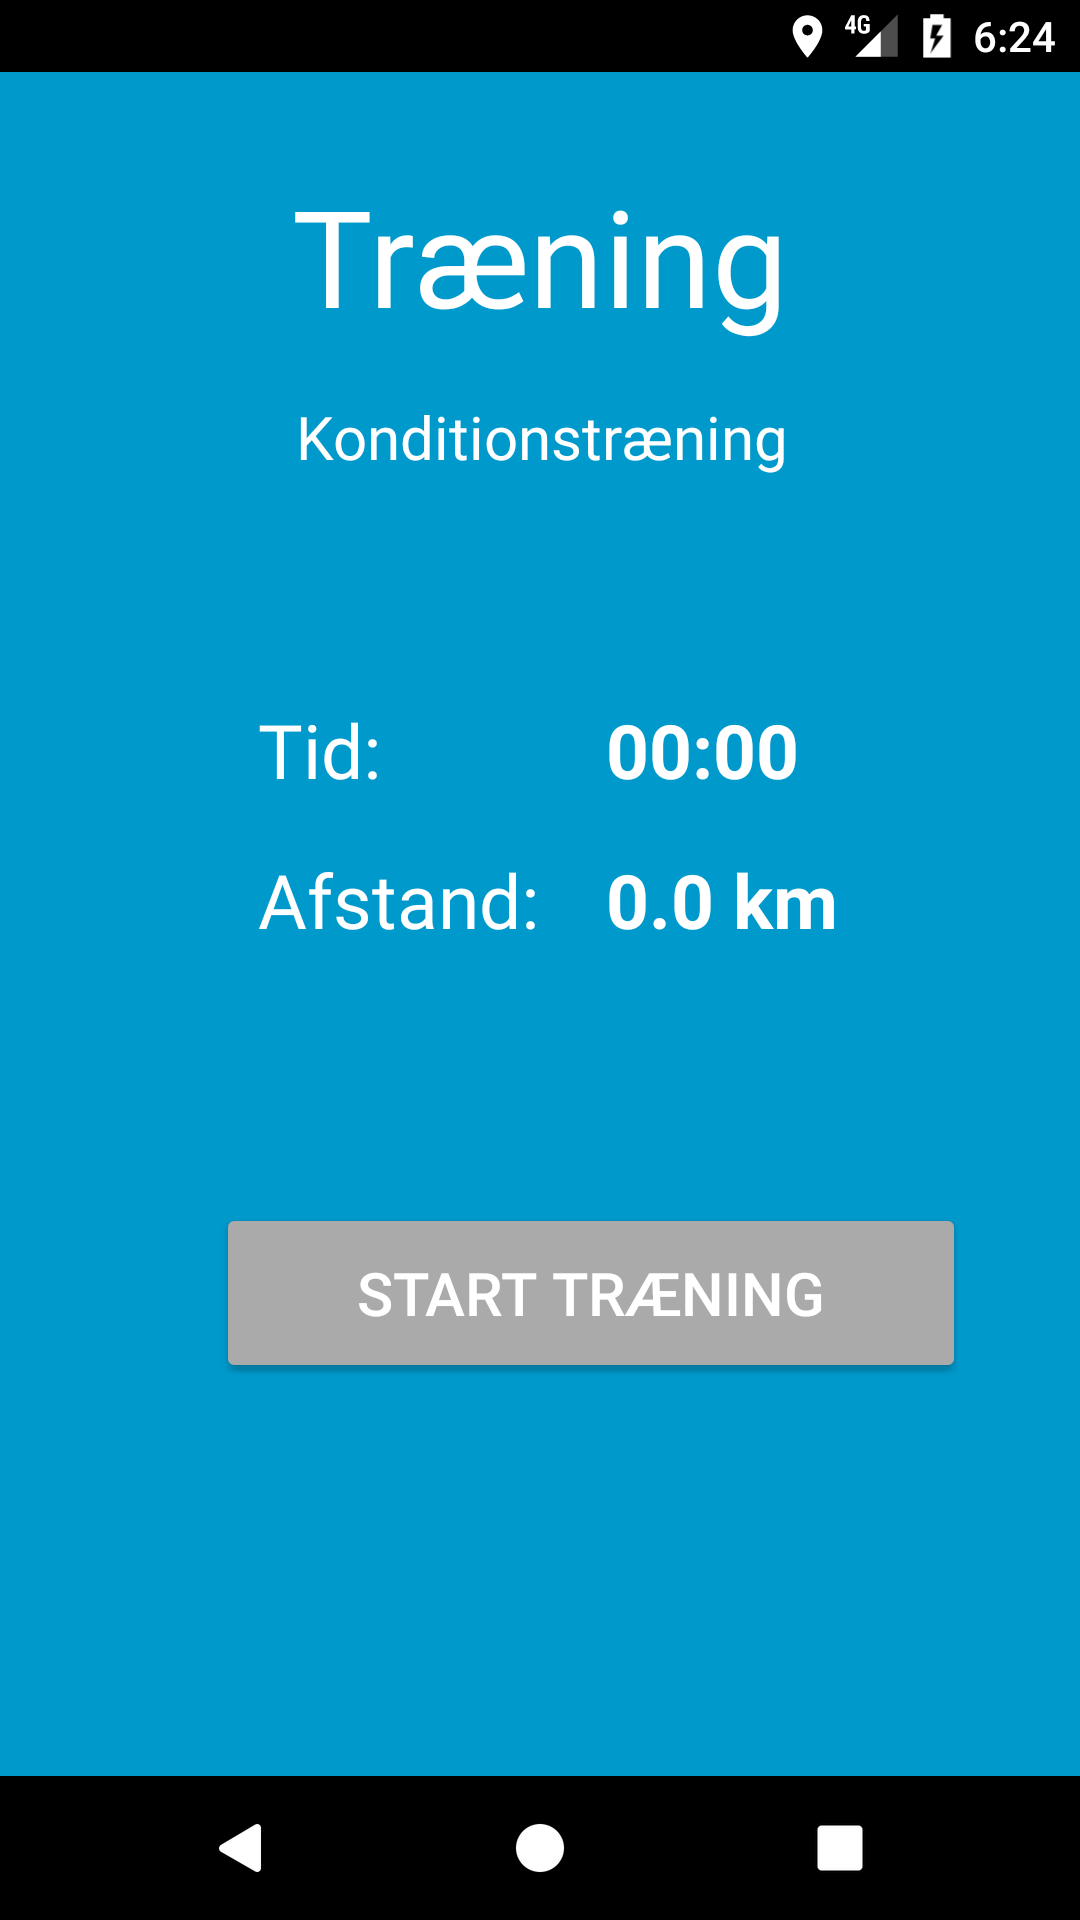
\includegraphics[width=0.24\textwidth, height=60mm]{figures/test/traening2}} 
      \hspace{5mm}
        \raisebox{-\totalheight}{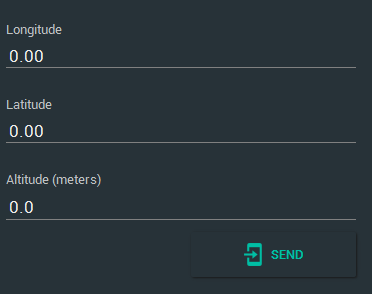
\includegraphics[width=0.24\textwidth, height=60mm]{figures/test/traening3}} 
      \hspace{5mm}
   \raisebox{-\totalheight}{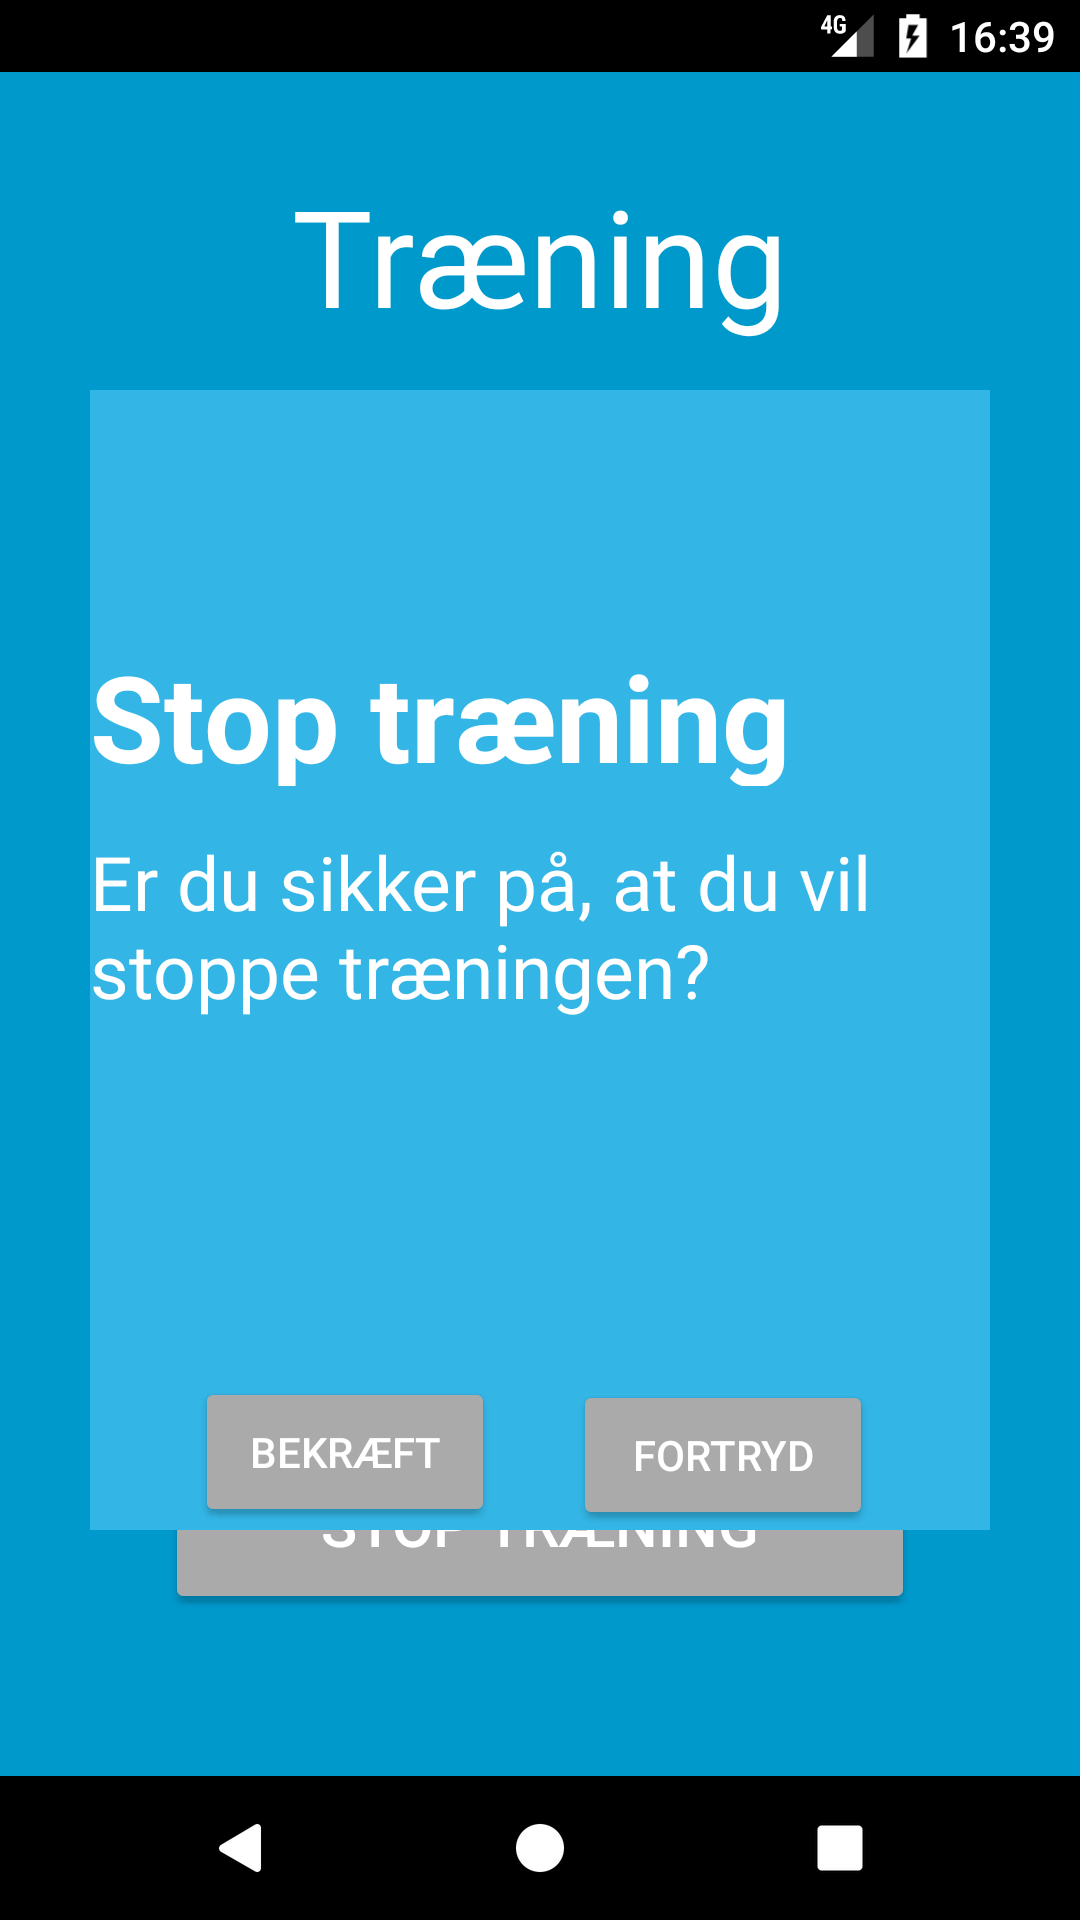
\includegraphics[width=0.24\textwidth, height=60mm]{figures/test/traening4}} 
     \vspace{3mm}
             ~~~~~~~~~~~ \textbf{\textit{Figur 1}}~~~~~~~~~~~~~~~~~~~~~~~~\textbf{\textit{Figur 2}}~~~~~~~~~~~~~~~~~~~~~~~~\textbf{\textit{Figur 3}}
    \newline
Resultater for det første main flow fremgår af ovenstående figurer. På venstre ses grænsefladen for træning før træningen er på begyndt. Når der trykkes på startknappen for træning, starter timer, som kan ses af den midterste figur. Til højre fremgår et popup-vindue, der indikerer, at træningen er stoppet.  \\ \hline
\textbf{Resultat main flow 2:} &  \hspace{1.5mm}
    \raisebox{-\totalheight}{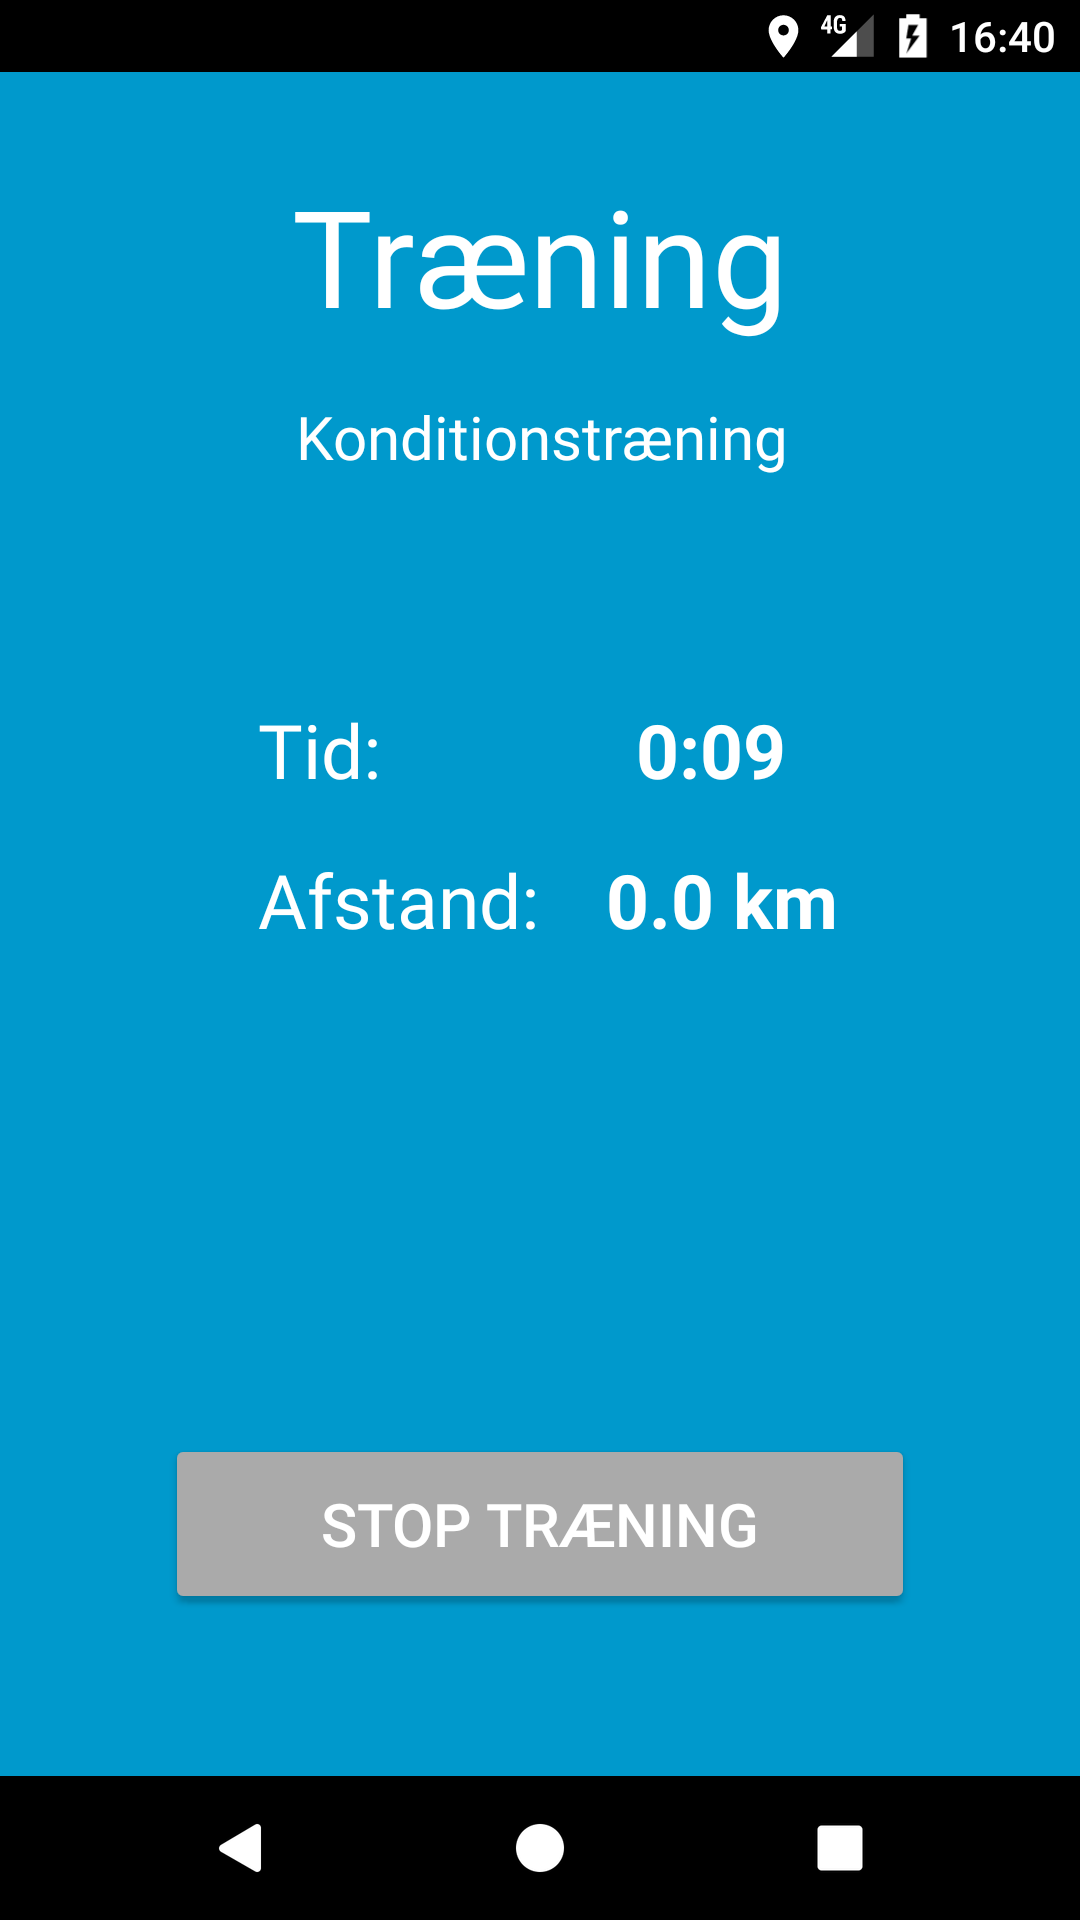
\includegraphics[width=0.24\textwidth, height=60mm]{figures/test/traening22}} 
      \hspace{5mm}
    \raisebox{-\totalheight}{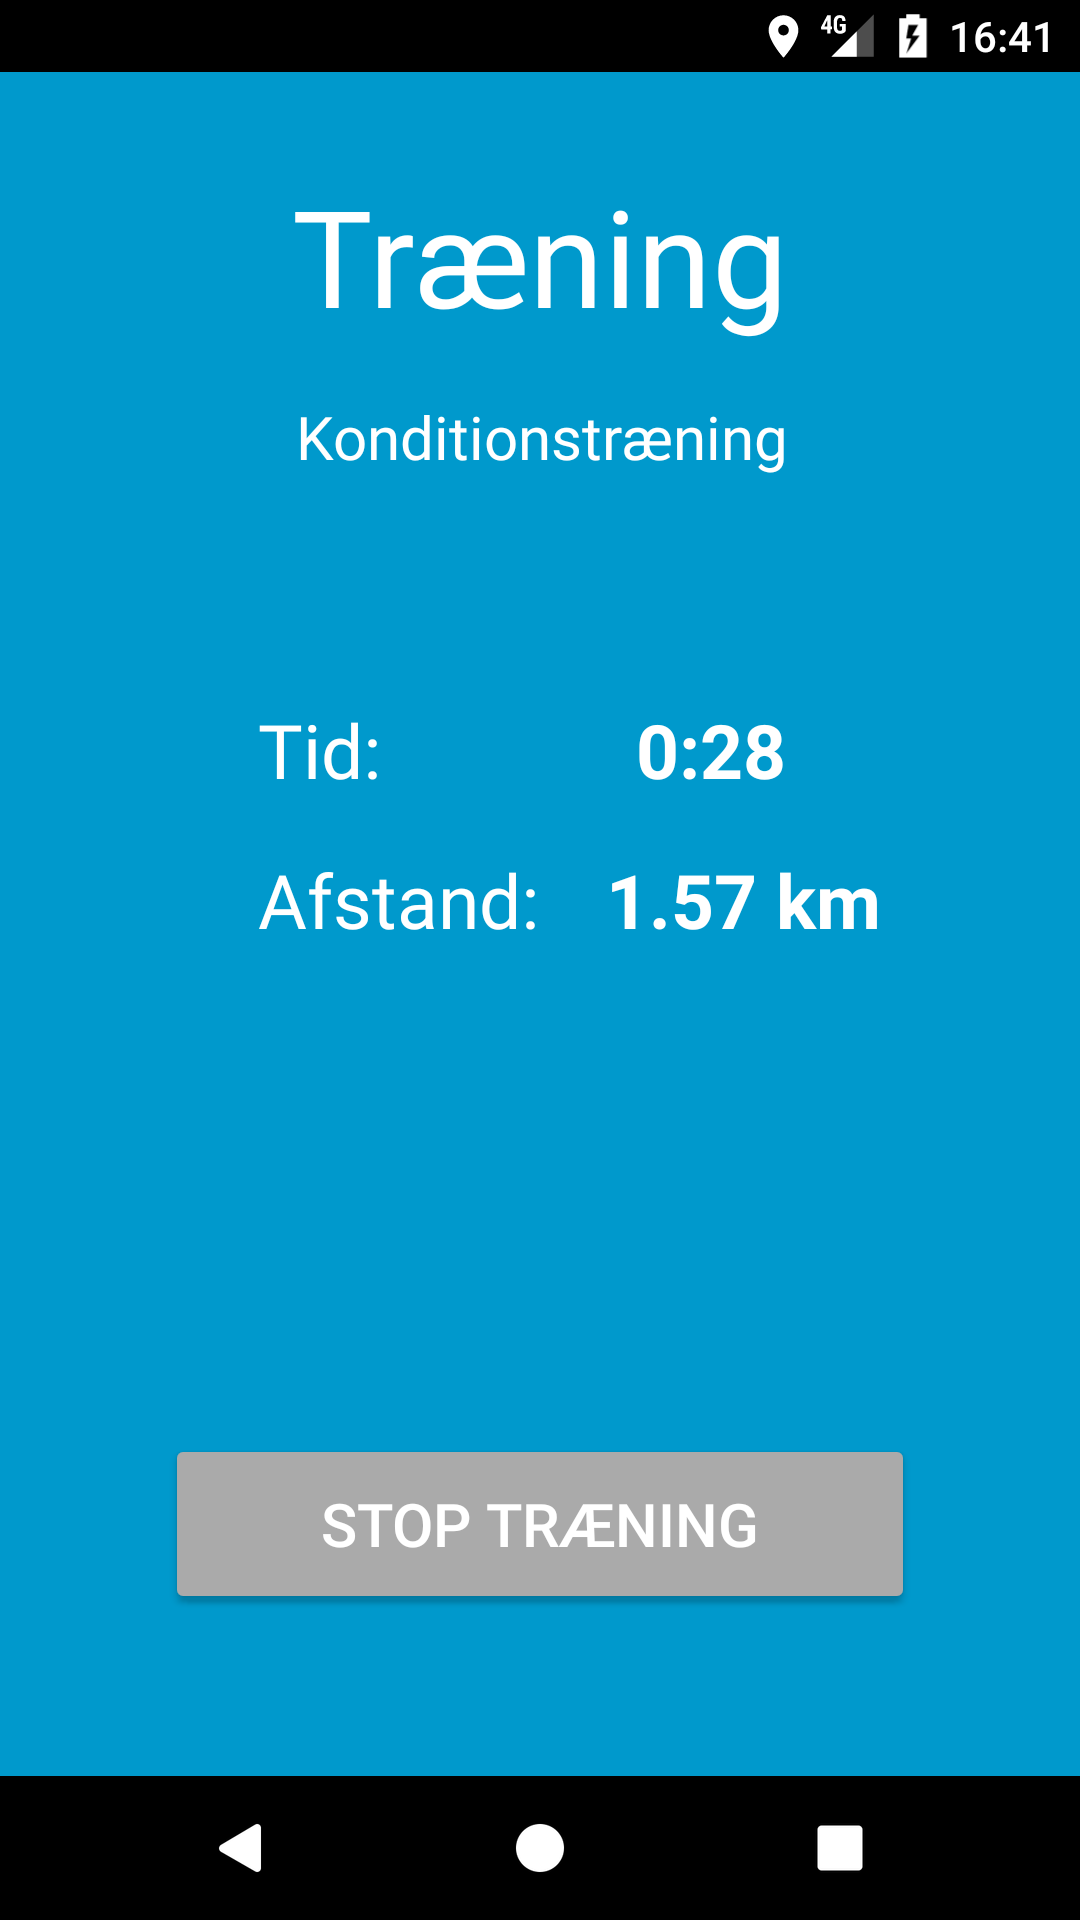
\includegraphics[width=0.24\textwidth, height=60mm]{figures/test/traening}} 
      \hspace{5mm}
   \raisebox{-\totalheight}{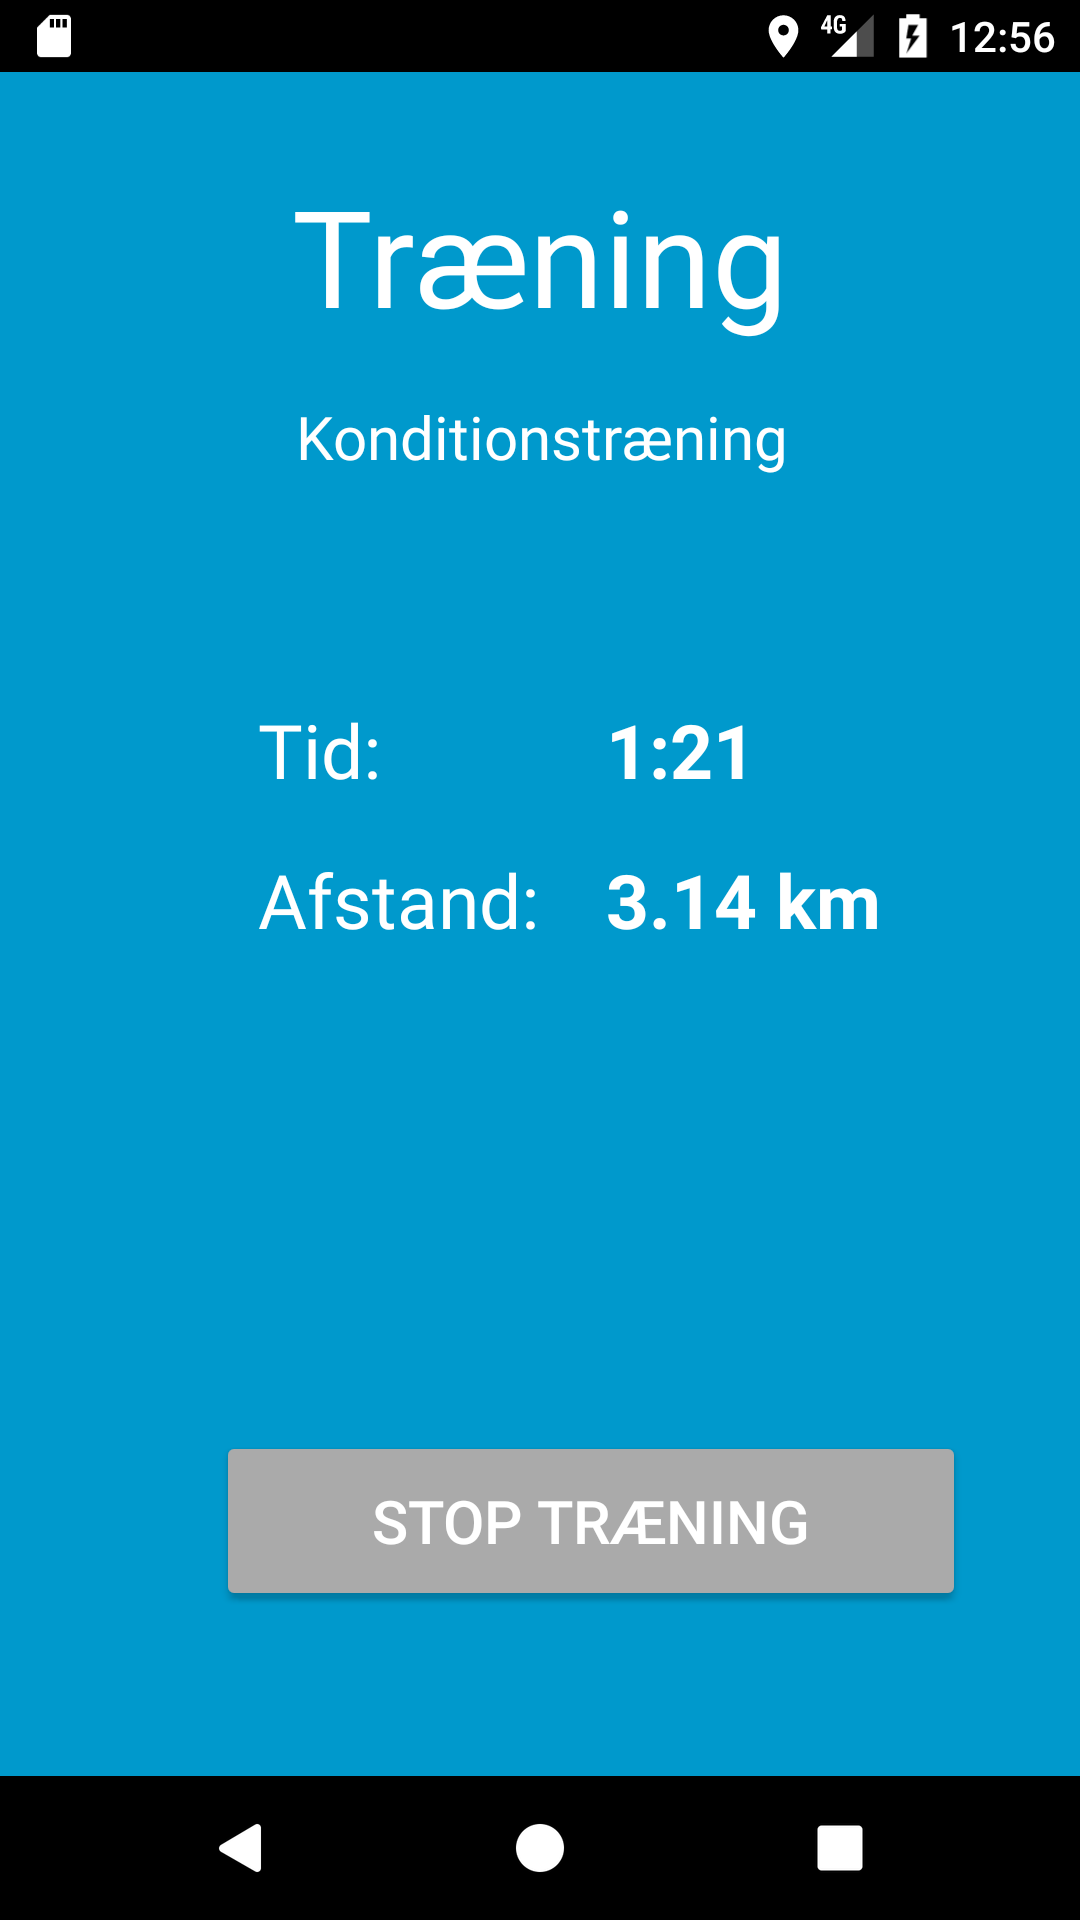
\includegraphics[width=0.24\textwidth, height=60mm]{figures/test/traening55}} 
   \vspace{3mm}
           ~~~~~~~~~~~ \textbf{\textit{Figur 4}}~~~~~~~~~~~~~~~~~~~~~~~~\textbf{\textit{Figur 5}}~~~~~~~~~~~~~~~~~~~~~~~~\textbf{\textit{Figur 6}}
    \newline
    Resultater for det andet main flow ses af ovenstående figurer. Til venstre ses grænsefladen for træningen, hvor det er simuleret, at brugeren har bevæget sig 0 km. I midten er det simuleret, at brugeren har bevæget sig 1.57 km. Til højre er det simuleret, at brugeren har bevæget sig 3.14 km. \\ \hline
\textbf{Resultat main flow 3:} &  \hspace{1.5mm}
    \raisebox{-\totalheight}{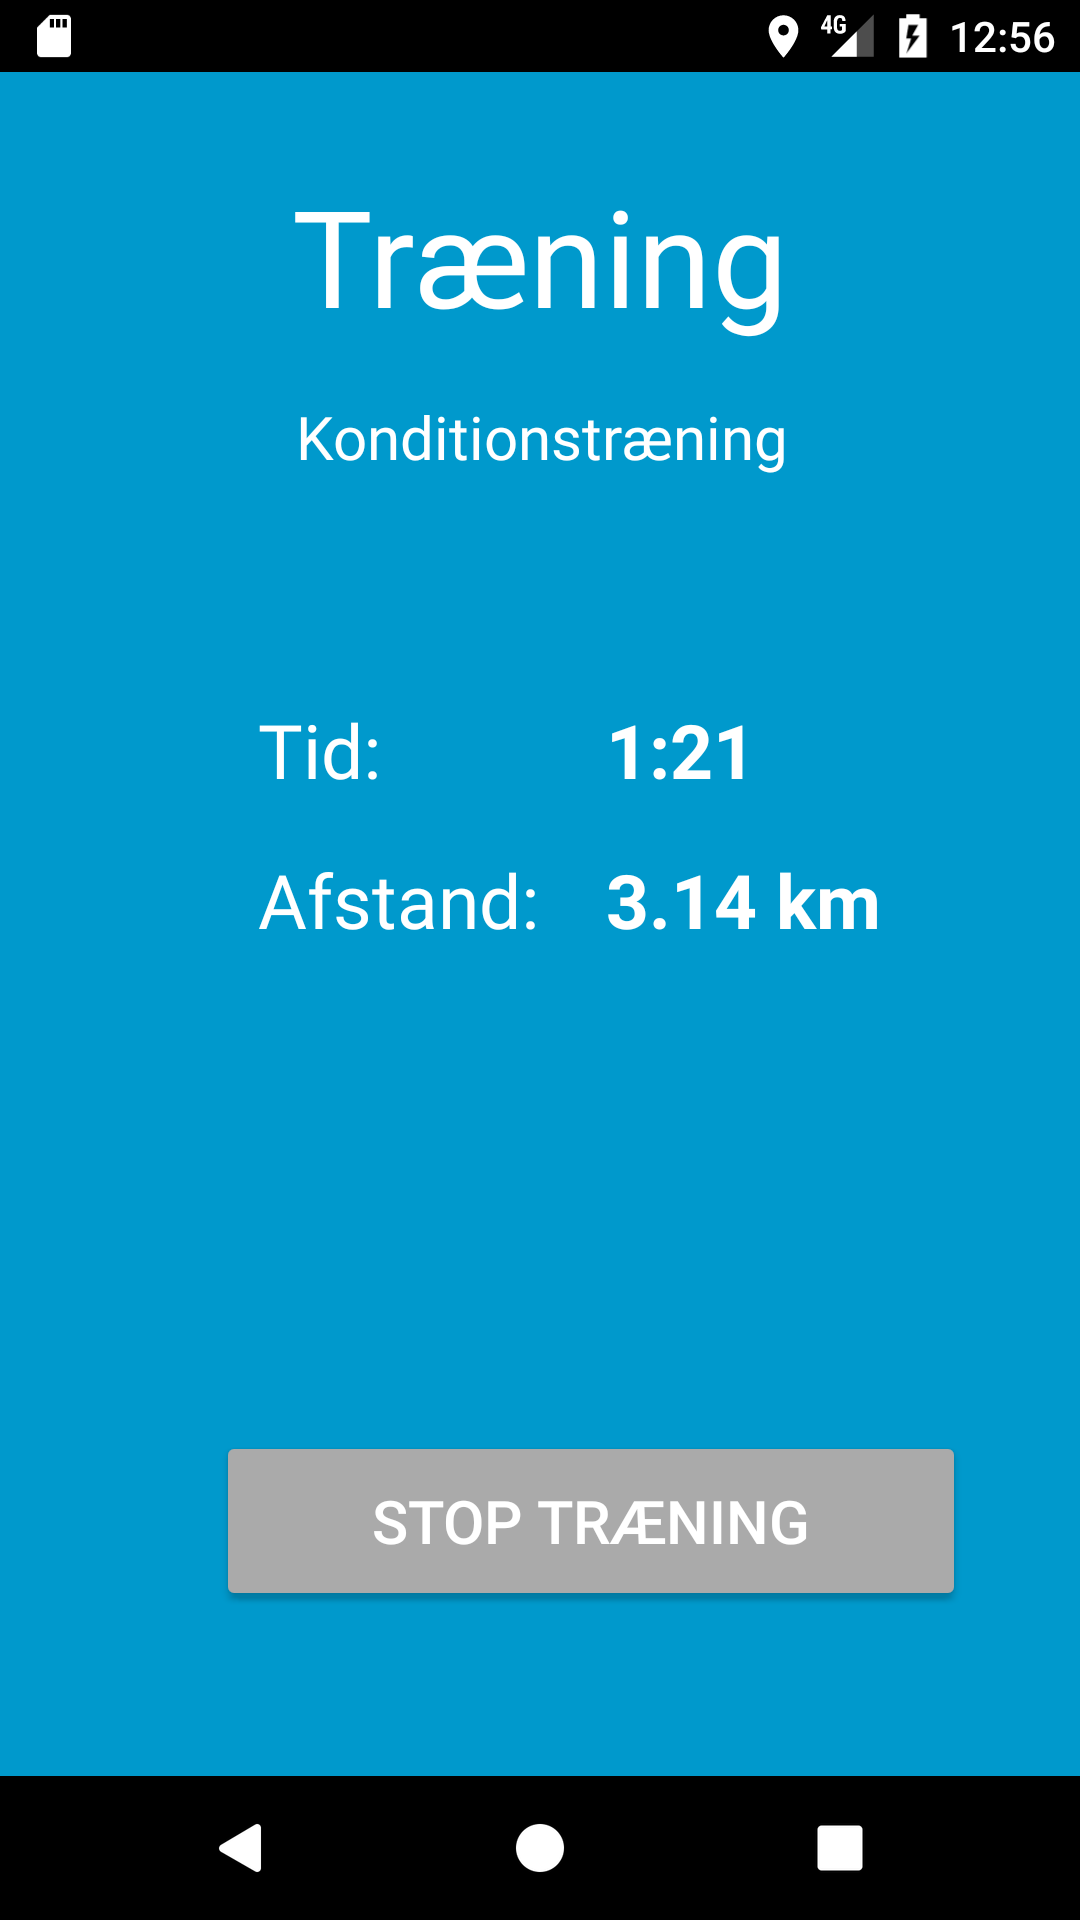
\includegraphics[width=0.24\textwidth, height=60mm]{figures/test/traening5}}
      \hspace{5mm}
             \raisebox{-\totalheight}{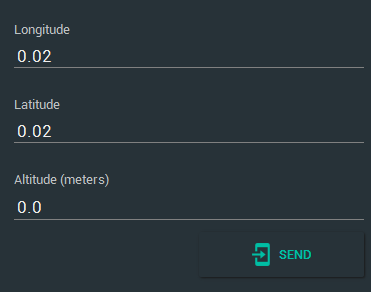
\includegraphics[width=0.24\textwidth, height=60mm]{figures/test/traening6}} 
      \hspace{5mm}
       \raisebox{-\totalheight}{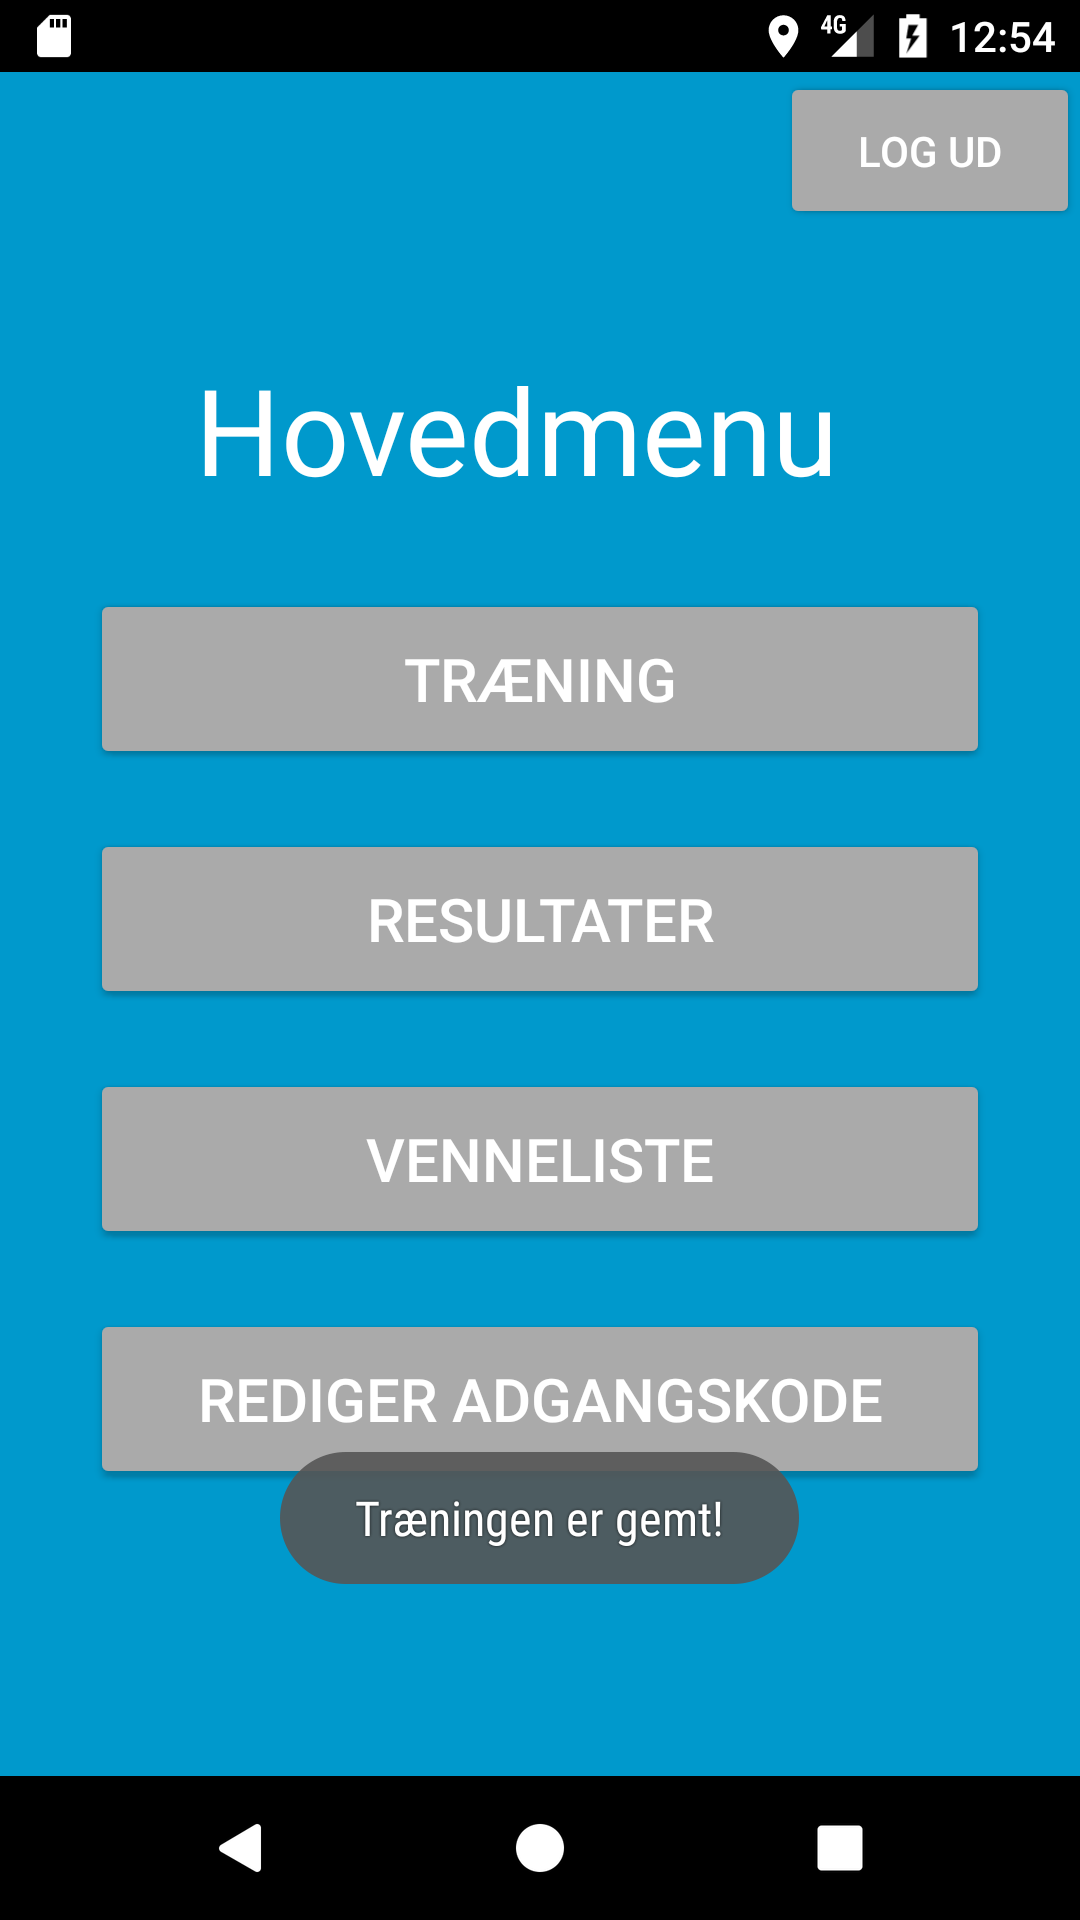
\includegraphics[width=0.24\textwidth, height=60mm]{figures/test/traening1}} 
   \vspace{3mm}
             ~~~~~~~~~~~ \textbf{\textit{Figur 7}}~~~~~~~~~~~~~~~~~~~~~~~~\textbf{\textit{Figur 8}}~~~~~~~~~~~~~~~~~~~~~~~~\textbf{\textit{Figur 9}}
    \newline
     Resultater for tredje main flow fremgår af ovenstående figurer. Til venstre og i midten ses evalueringen, der fremkommer efter udført træning. Figuren i midten viser, at brugeren har angivet evaluering, idet videreknappen er synlig. På figuren til højre fremgår det, at træningen er gemt, hvormed evalueringen for træningen ligeledes er gemt.  
     \\ \hline
 \textbf{Resultat main flow 4:} & \hspace{0.3mm}
  \raisebox{-\totalheight}{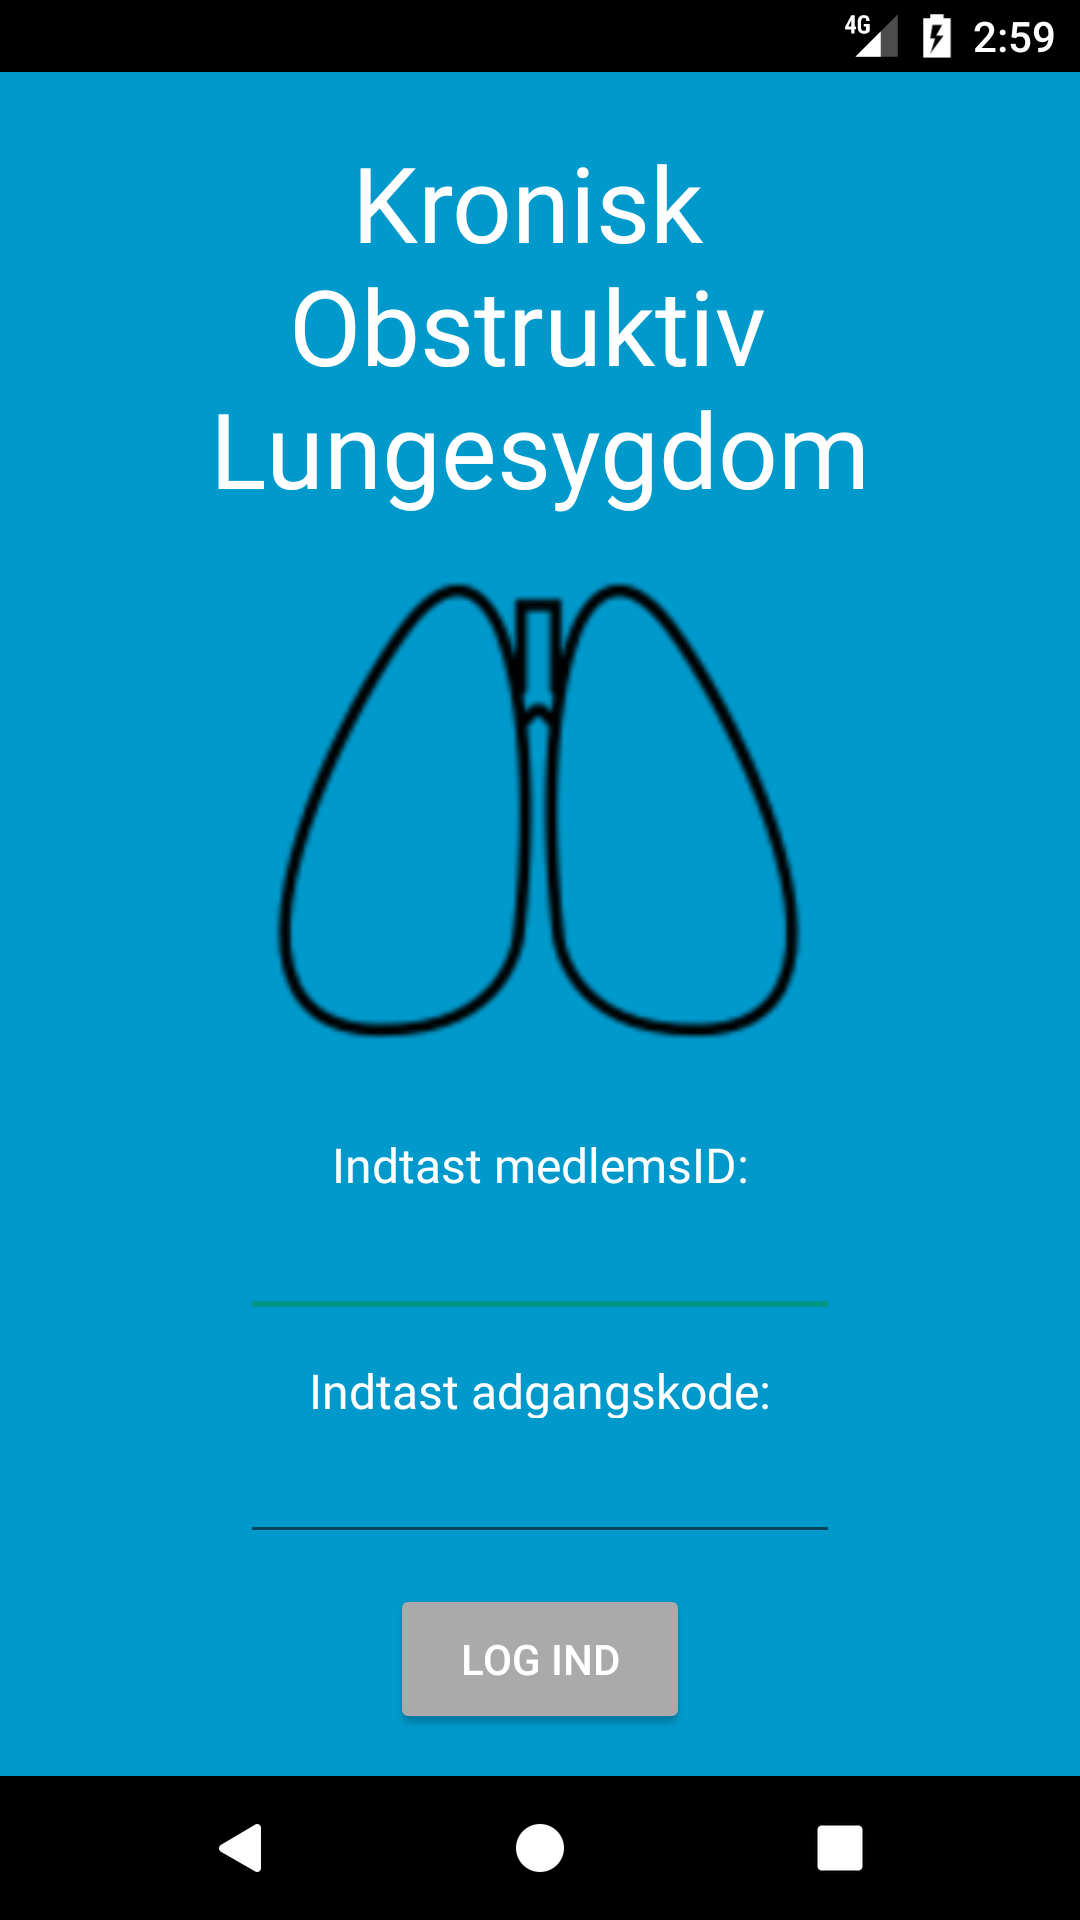
\includegraphics[width=0.20\textwidth, height=60mm]{figures/test/notification1}} 
   \raisebox{-\totalheight}{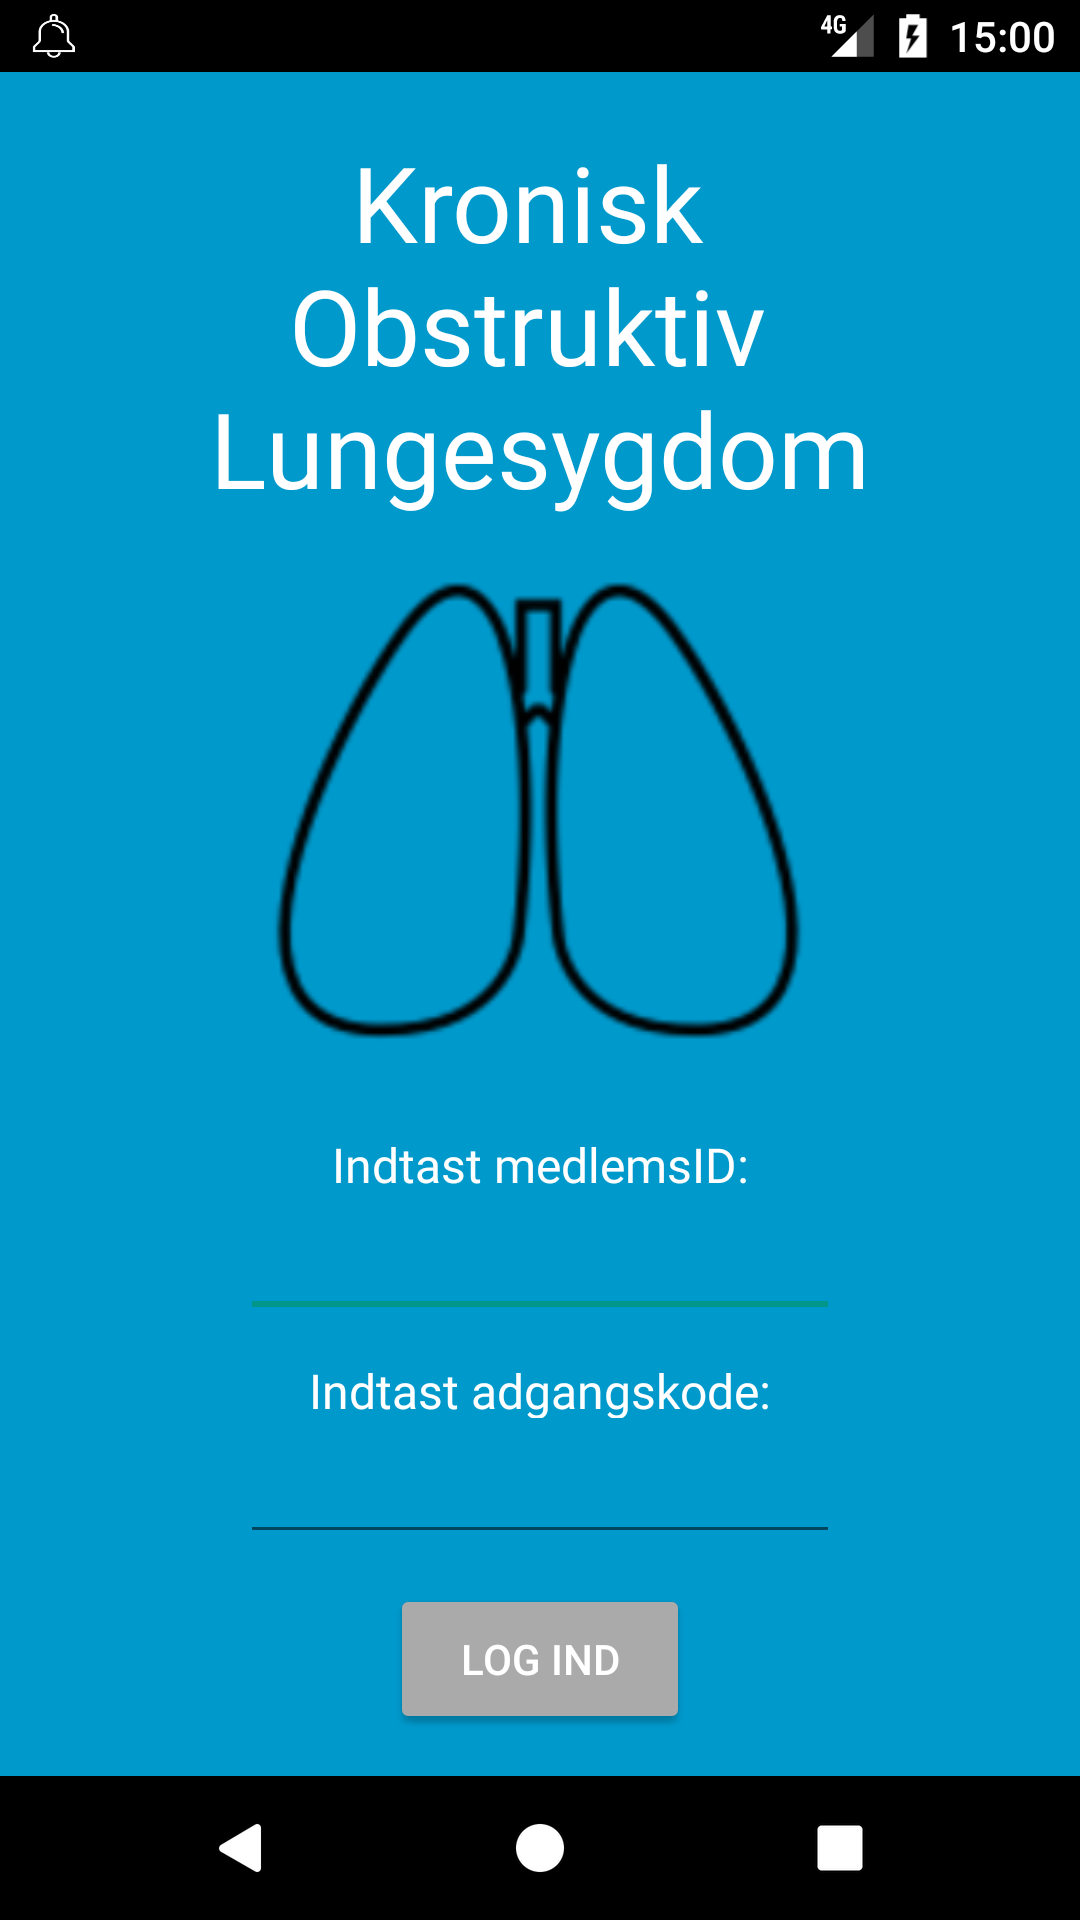
\includegraphics[width=0.20\textwidth, height=60mm]{figures/test/notification2}} 
    \raisebox{-\totalheight}{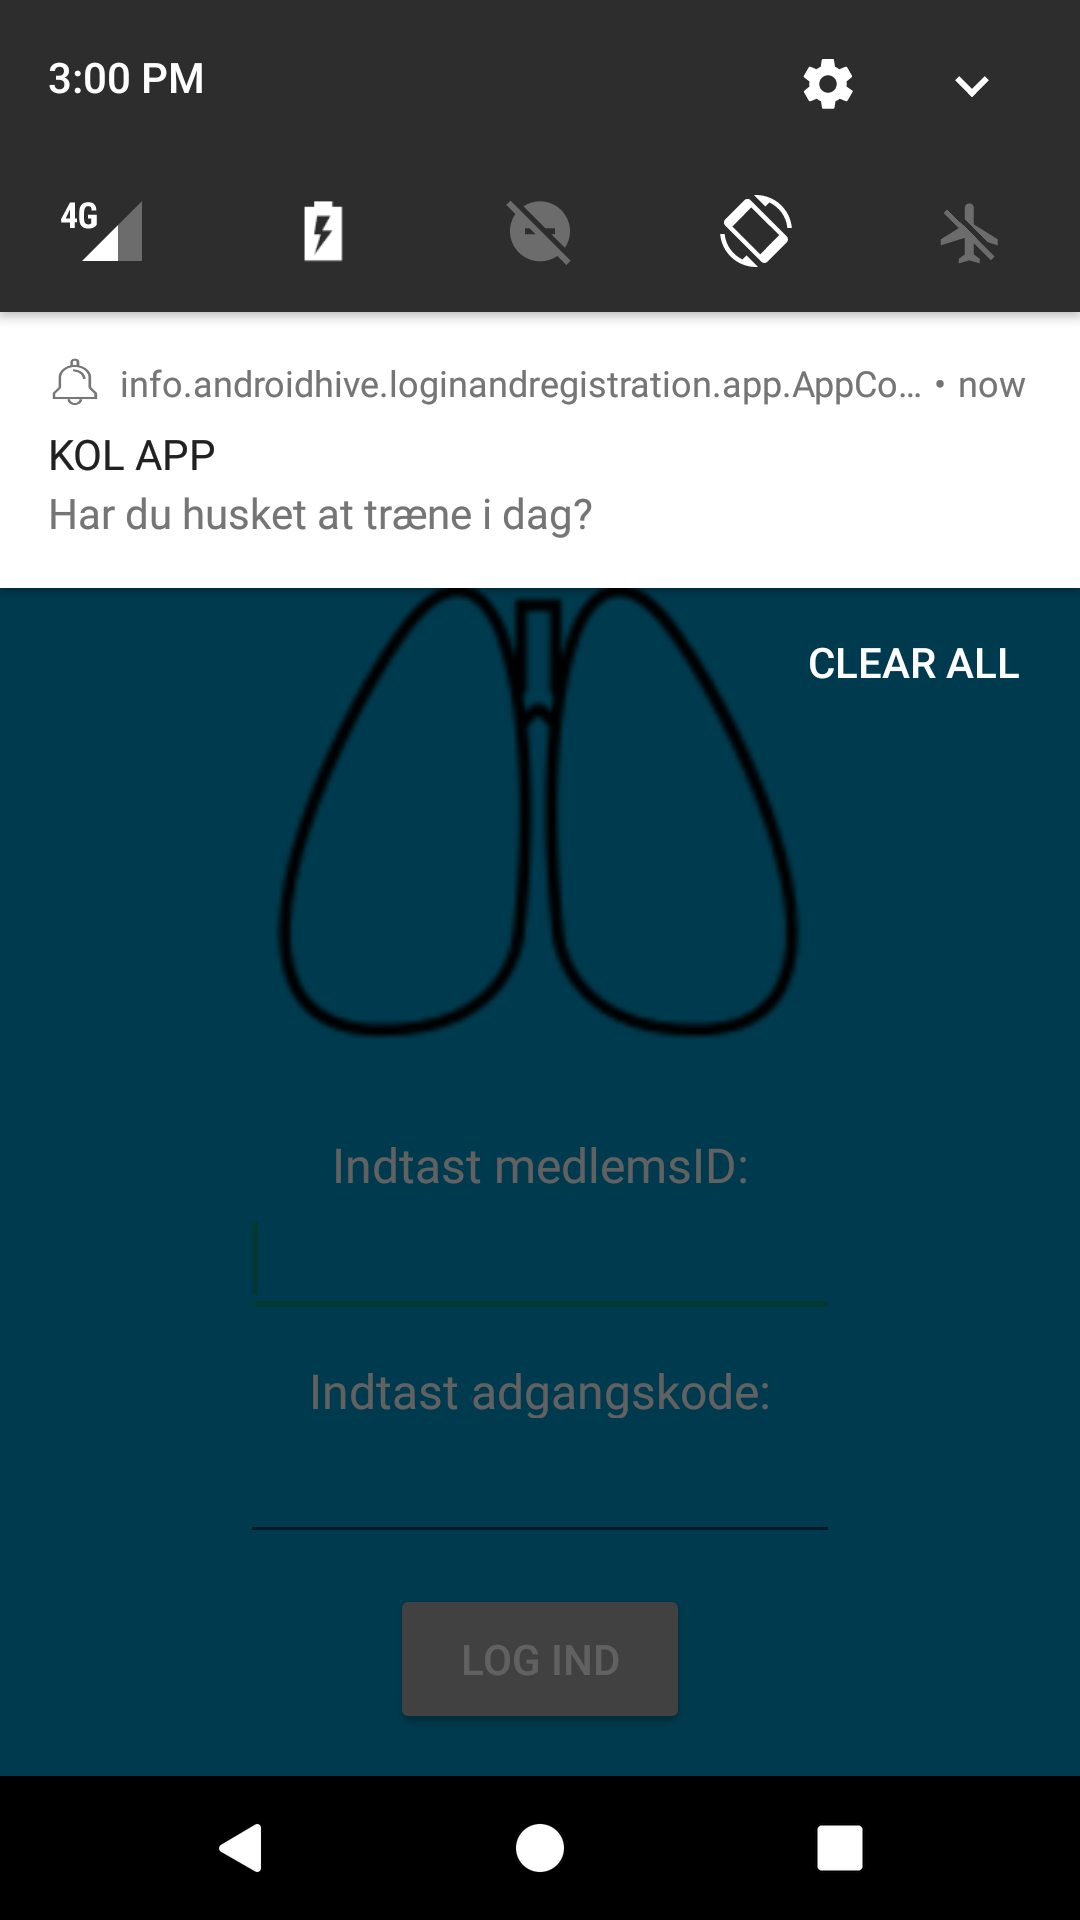
\includegraphics[width=0.20\textwidth, height=60mm]{figures/test/notification3}} 
 \raisebox{-\totalheight}{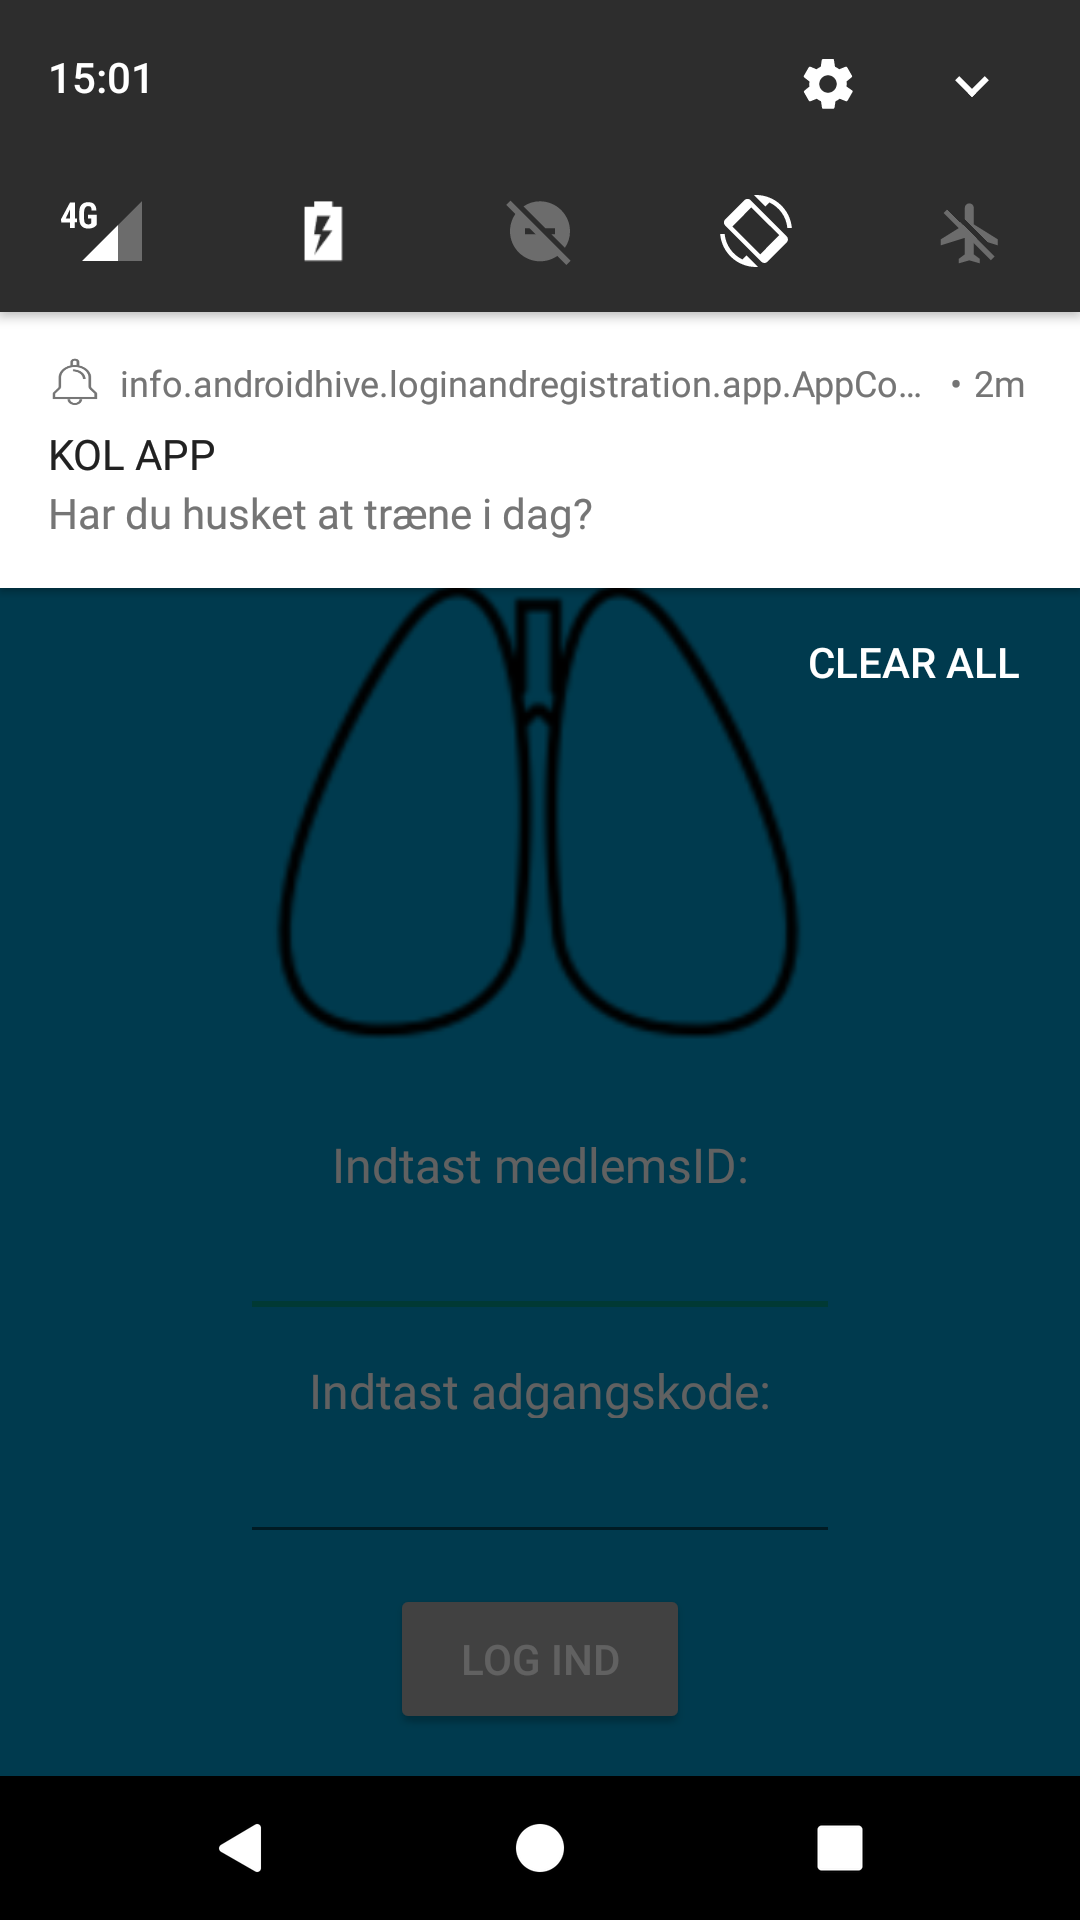
\includegraphics[width=0.20\textwidth, height=60mm]{figures/test/notification4}} 
    \vspace{3mm}
          ~~~~~~~~\textbf{\textit{Figur 10}}~~~~~~~~~~~~\textbf{\textit{Figur 11}}~~~~~~~~~~~~\textbf{\textit{Figur 12}}~~~~~~~~~~~~~\textbf{\textit{Figur 13}}
    \newline
     Resultater for fjerde main flow fremgår af ovenstående figurer. I de to midterste figurer ses det at notifikationen, i øverste venstre hjørne, er startet klokken 15. Udvides notifikationen, ved at slide topbaren ned, ses denne som vist af figuren til højre.
     \\ \hline
\textbf{Resultat:} &
    \begin{itemize}[label={\checkmark}]
\item På baggrund af resultater for main flow er kravene for træning opfyldt
\end{itemize} \\ \hline
  % \end{tabular}
   \caption{Test af træning.}
    \label{tab:testTraening}
\end{longtable}


\section{Resultater}
Resultater skal motivere brugeren til at udføre træningen. Følgende krav er opstillet for resultater:
\begin{itemize}
\item Systemet skal kunne vise brugerens ugentlige træningsudvikling
\\
\textit{Dette er nødvendigt for, at brugere kan følge sin ugentlige udvikling samt motivere brugeren}
\item Systemet skal kunne give virtuelle belønninger
\\
\textit{Dette er nødvendigt for at kunne motivere brugere til at udføre træning}
\end{itemize}

\noindent
For at teste om de opstillede krav til resultater er overholdt, udføres testen, der fremgår af \autoref{tab:testResultater}.
  \begin{longtable}{ | l | p{13cm} |} \hline
    \textbf{Test:} & Resultater \\ \hline
  \textbf{Formål:} & Formålet er, at systemet skal kunne vise den ugentlige træningsudvikling grafisk samt give virtuelle belønninger efter \autoref{tab:SamletBelon}. Dette gøres ved at træne imens, der måles tid og afstand. 
 \\ \hline
 	\textbf{Main flow:} & 1.~Tryk på \textit{TRÆNING} via hovedmenu. \textit{START TRÆNING} og vent 120 minutter. Imens åbnes Extended controls og sæt longitude samt latitude til 0 og tryk send. Ændre herefter til 0.16. Tryk \textit{STOP TRÆNING} og evaluer træningen til \textit{:-D}. Tryk herefter på \textit{RESULTATER} via hovedmenuen og vælg \textit{BELØNNINGER}. 
 	\begin{itemize} 
 	\item Grafen viser, at brugeren har trænet 120 minutter på en enkelt dag (\textbf{\textit{Figur 3}})
 	\item Brugeren har opnået én stjerne i kategorien antal træninger (\textbf{\textit{Figur 4}})
 	\item Brugeren har opnået tre stjerner i kategorien tid (\textbf{\textit{Figur 4}})
  	\item Brugeren har opnået to stjerner i kategorien afstand (\textbf{\textit{Figur 4}})
    \item Brugeren har opnået én stjerne i kategorien konditionstræning (\textbf{\textit{Figur 4}})
  \end{itemize}
\\ \hline
\textbf{} & \hspace{0.3mm}
  \raisebox{-\totalheight}{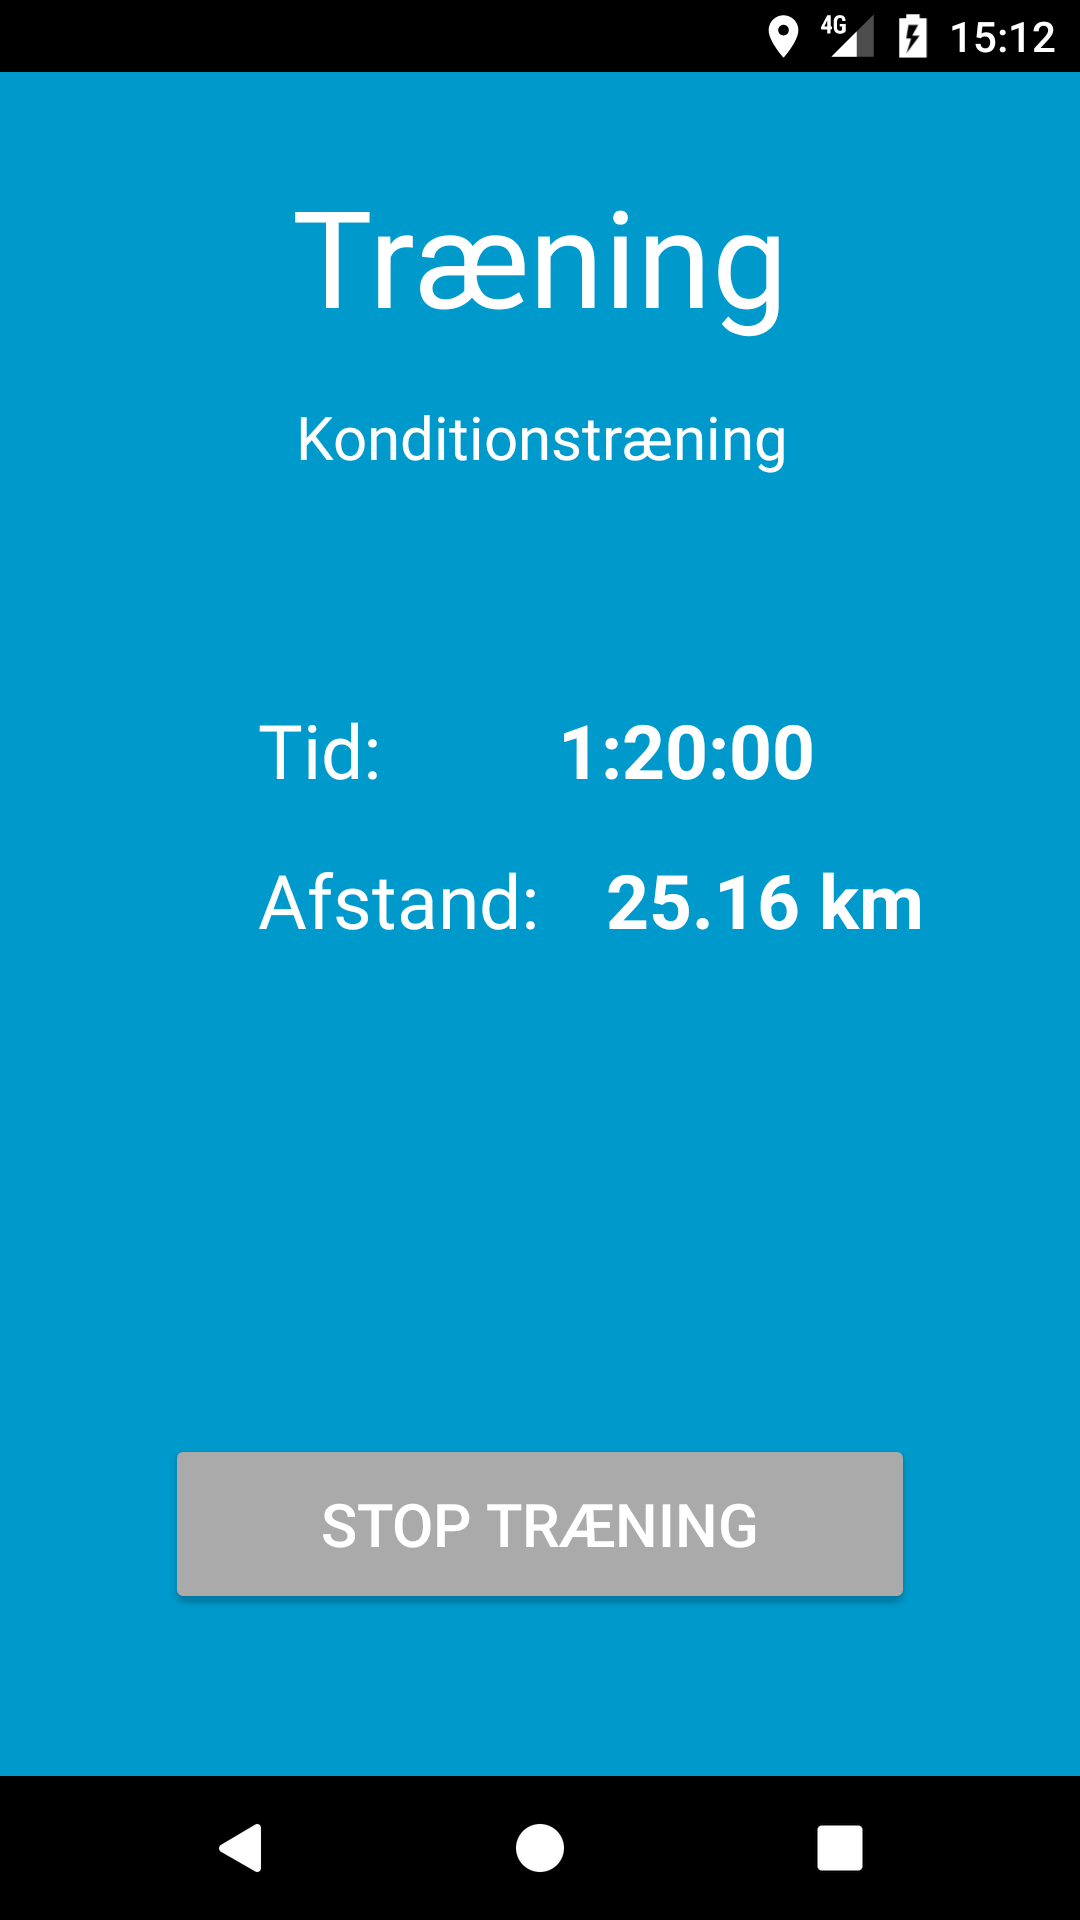
\includegraphics[width=0.20\textwidth, height=60mm]{figures/test/result}} 
   \raisebox{-\totalheight}{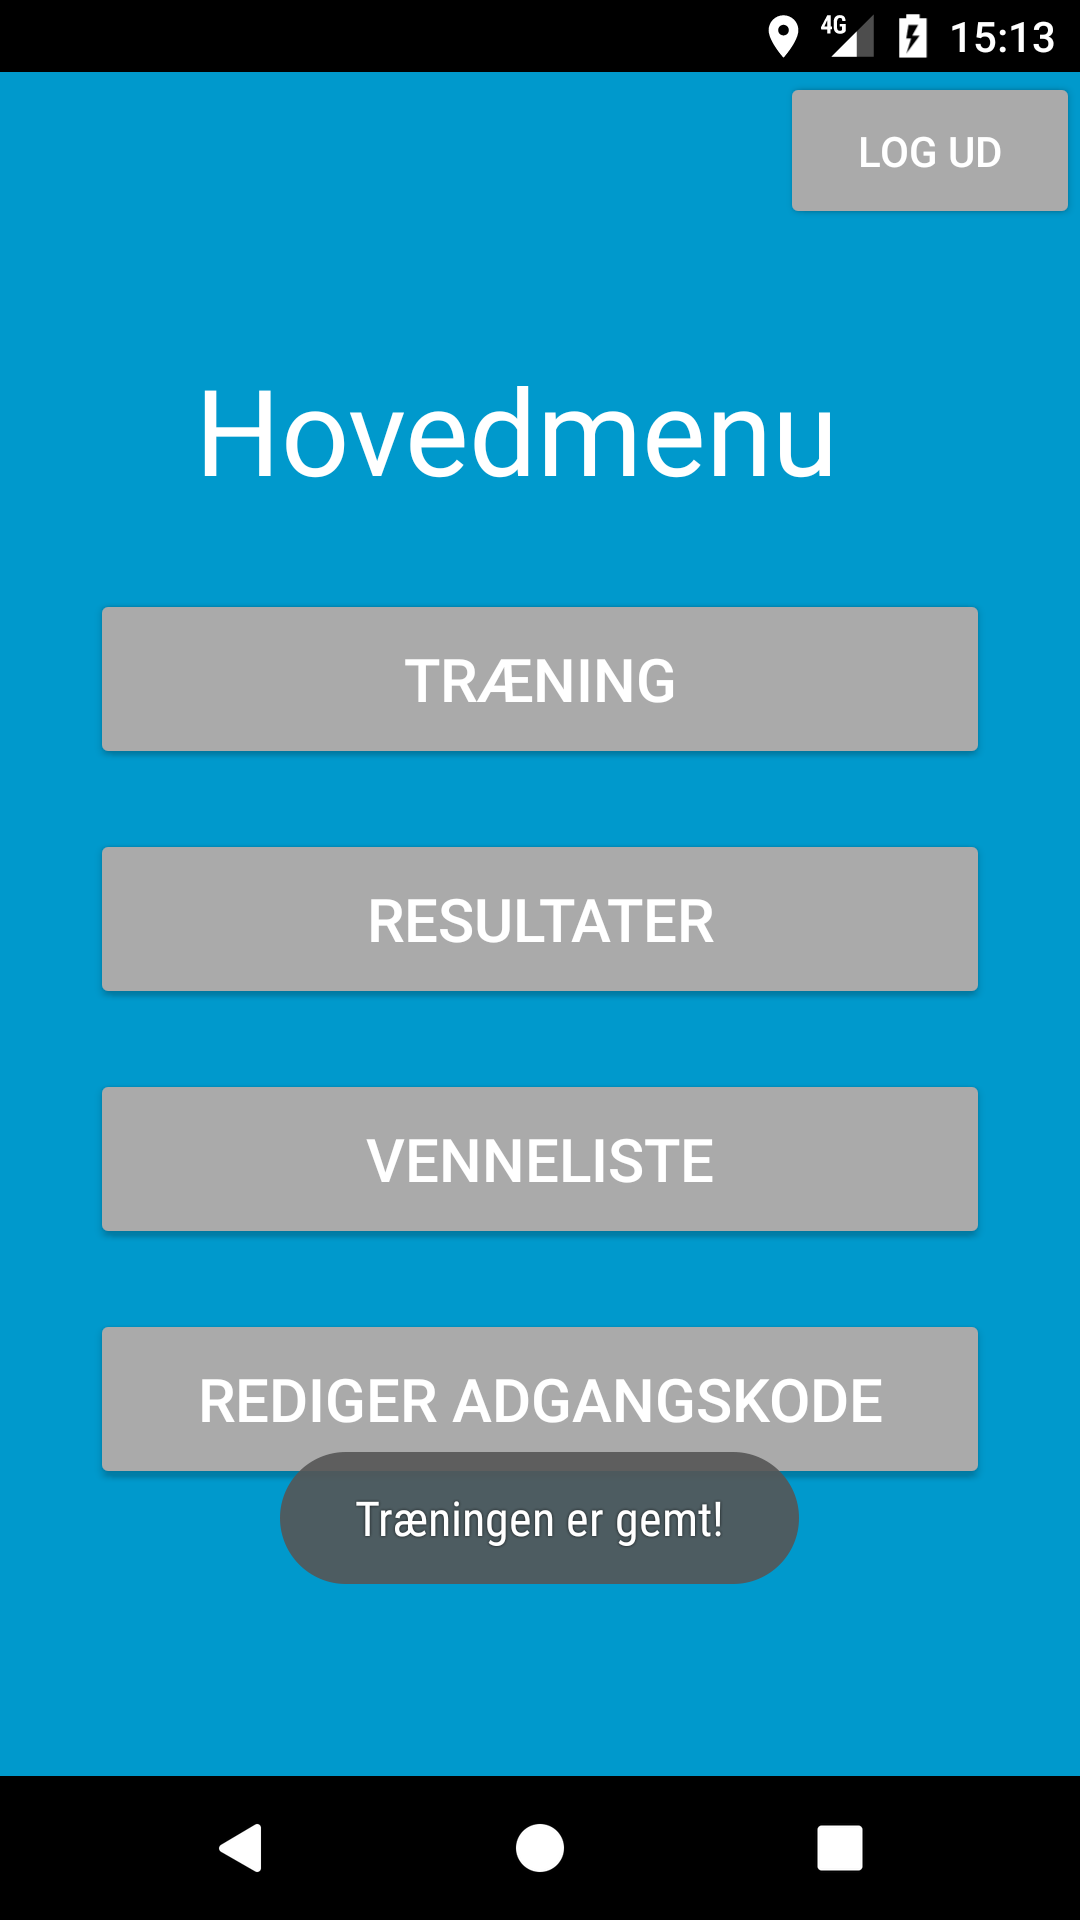
\includegraphics[width=0.20\textwidth, height=60mm]{figures/test/result1}} 
    \raisebox{-\totalheight}{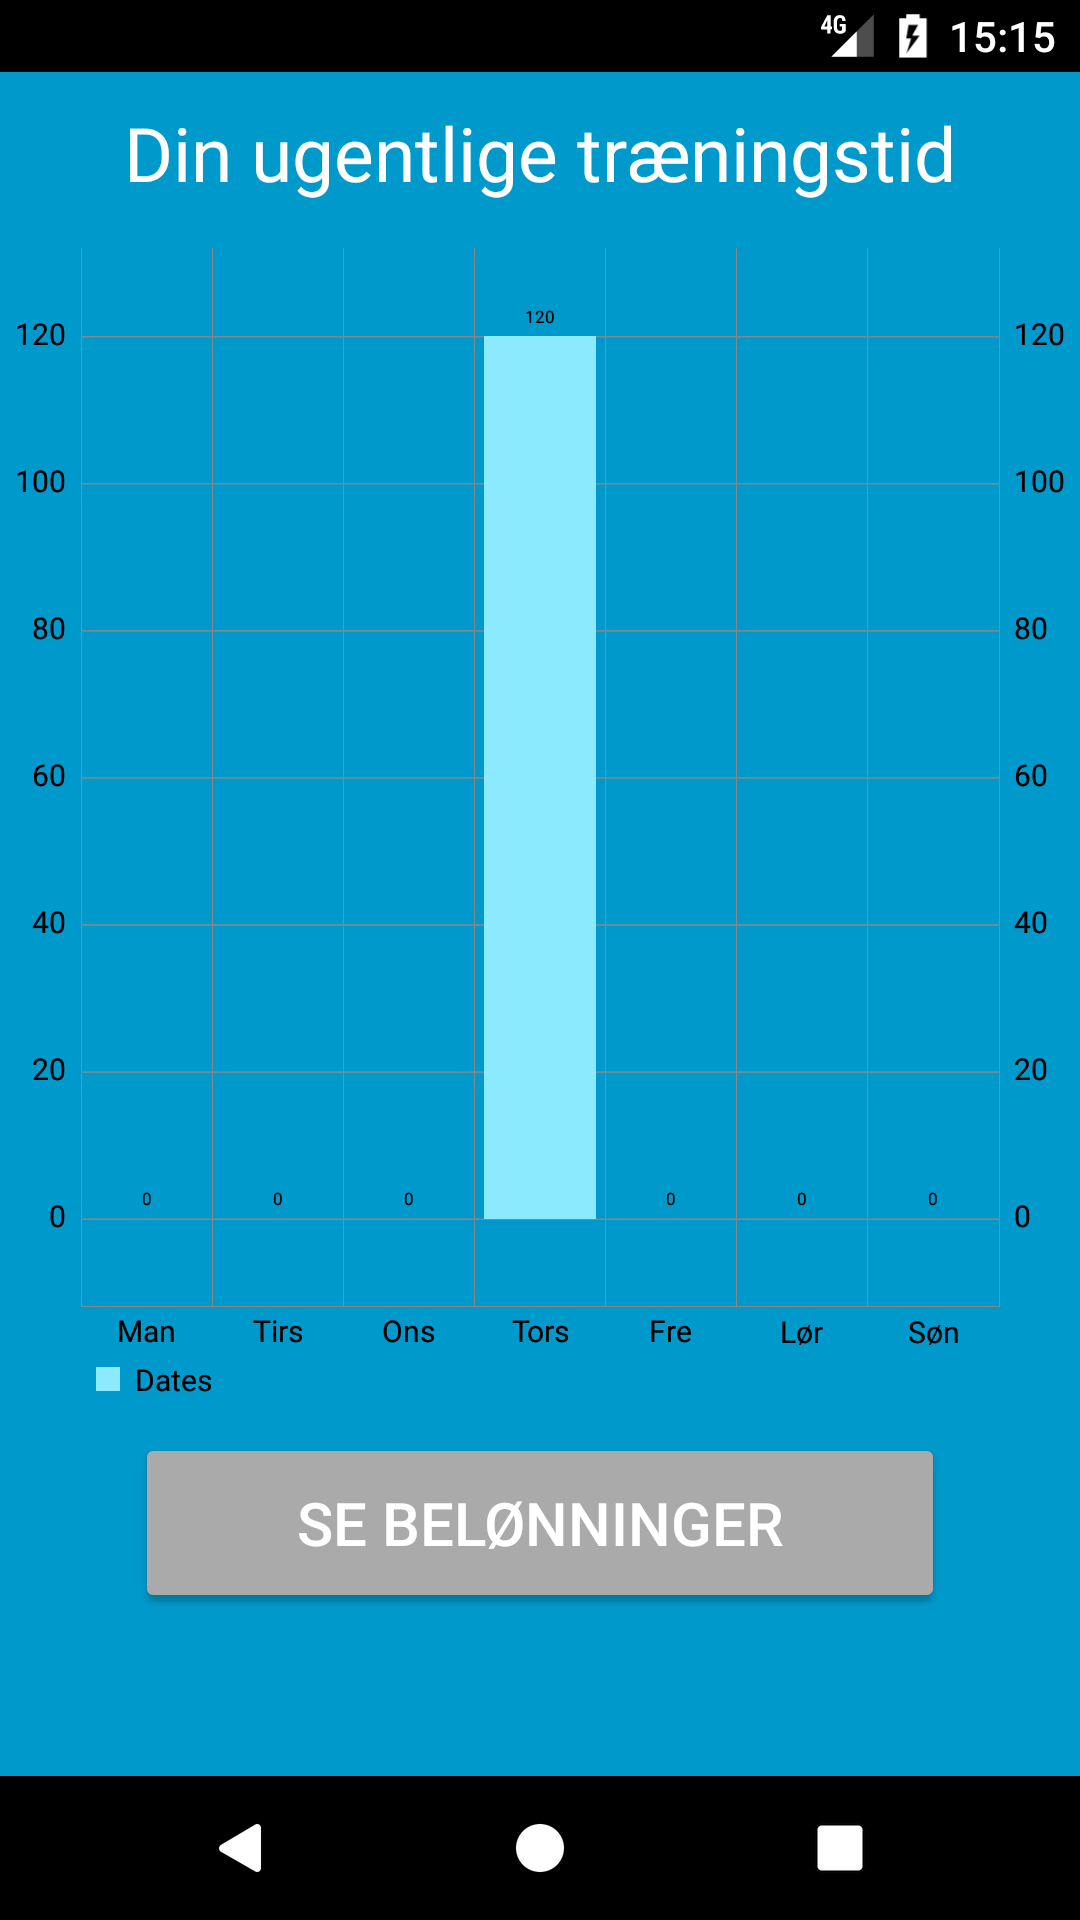
\includegraphics[width=0.20\textwidth, height=60mm]{figures/test/result2}} 
 \raisebox{-\totalheight}{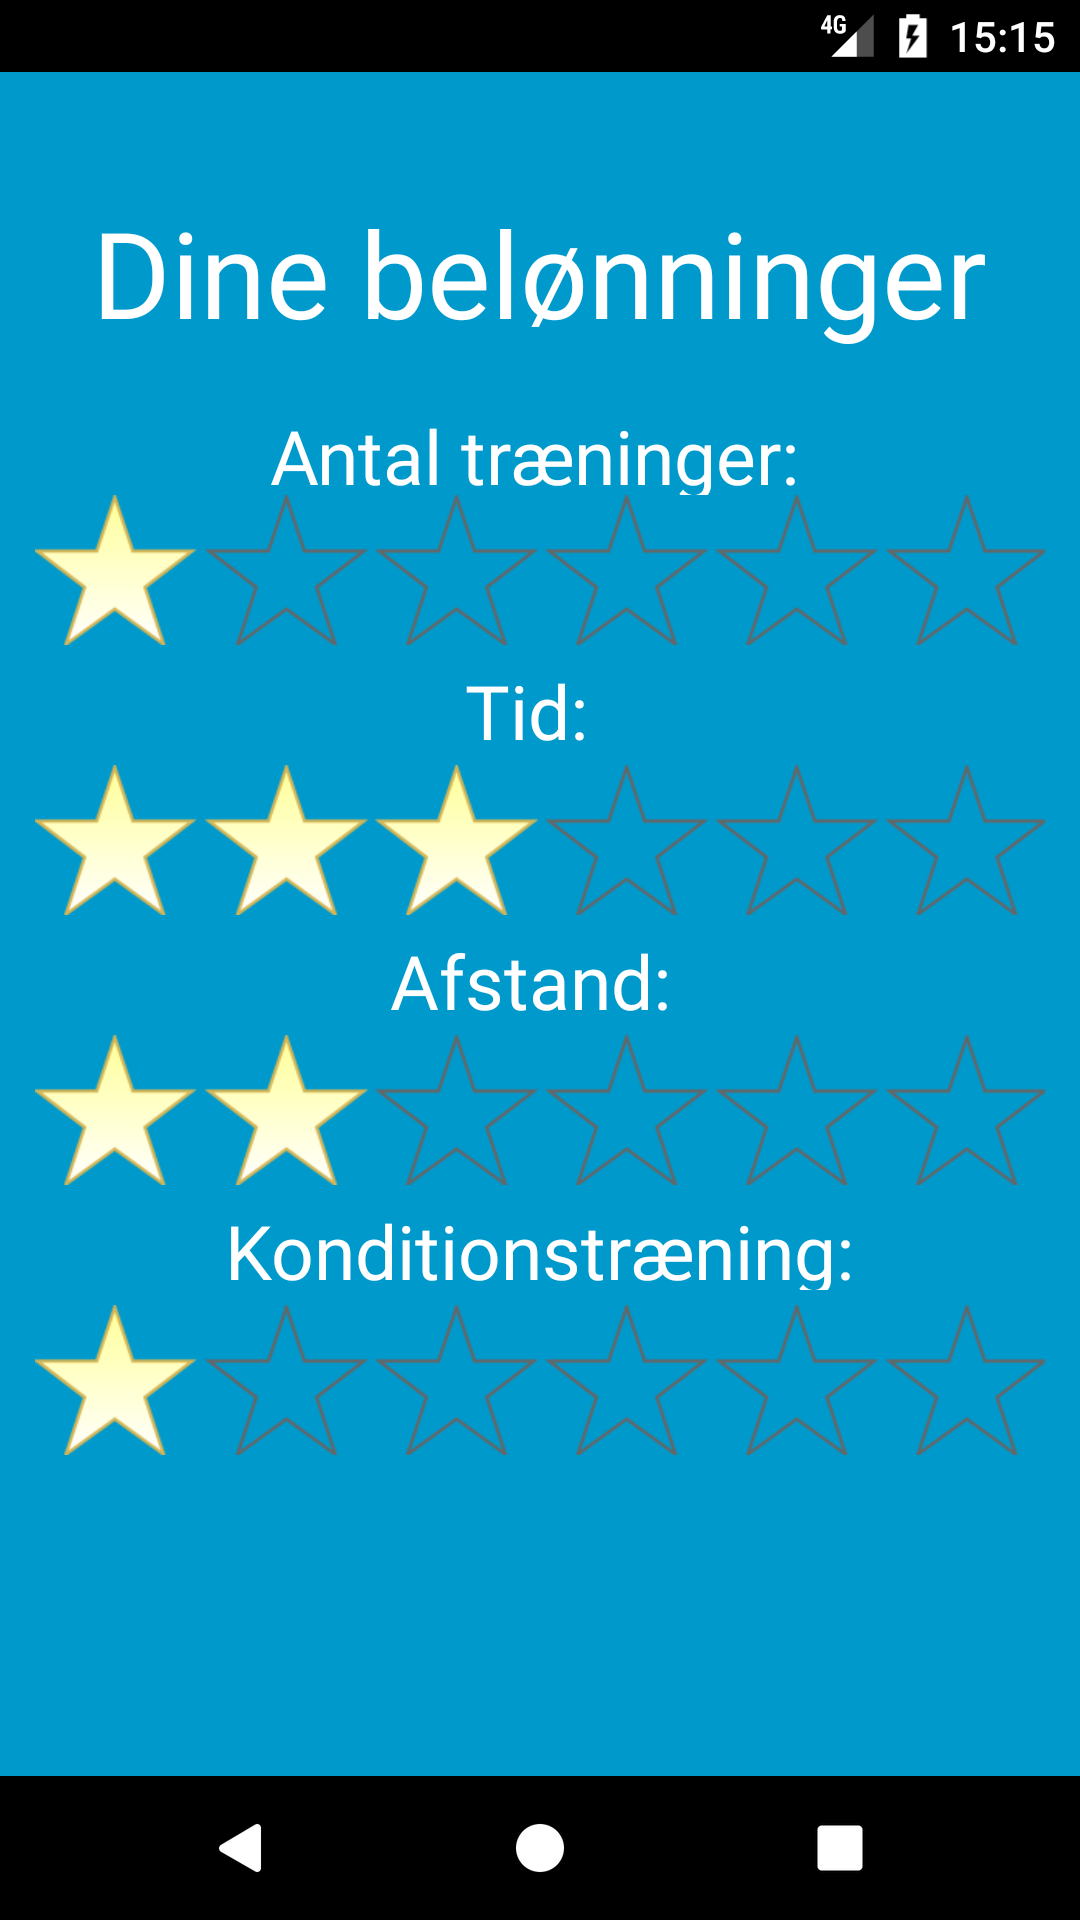
\includegraphics[width=0.20\textwidth, height=60mm]{figures/test/result3}} 
    \vspace{3mm}
          ~~~~~~~~\textbf{\textit{Figur 1}}~~~~~~~~~~~~~~\textbf{\textit{Figur 2}}~~~~~~~~~~~~~~~\textbf{\textit{Figur 3}}~~~~~~~~~~~~~~\textbf{\textit{Figur 4}}
    \newline
På figurerne ovenfor vises resultaterne for test af resultater. Til venstre fremgår den ønskede tid og afstand. Anden figur viser, at resultaterne fra træningen gemmes, hvoraf figuren til højre for denne viser grafisk udvikling af den ugentlige træningstid. Den fjerde figur viser belønninger, der er visualiseret som stjerner. De opnåede stjerner afspejler, at brugeren har udført det antal træninger svarende til de opnåede stjerner. 
  \begin{itemize}[label={\checkmark}]
\item På baggrund af denne test er kravet for resultater opfyldt
\end{itemize}
    \\ \hline
   \caption{Test af resultater.}
    \label{tab:testResultater}
\end{longtable}

\section{Venneliste}
Vennelisten skal give en fællesskabsfølelse for brugeren ved at kunne følge og kunne tilgå andre brugeres virtuelle belønninger. Derudover skal vennelisten motivere brugeren til at udføre træning. Følgende krav er opstillet til vennelisten: 

\begin{itemize}
\item Brugere skal kunne følge andre brugere
\\
\textit{Dette er nødvendigt for at skabe fællesskab samt gøre det muligt for brugere at tilgå hinandens virtuelle belønninger, hvilket skal øge brugeres motivation}
\end{itemize}

\noindent
Der testes, om ovenstående krav til vennelisten er opfyldt. Testen fremgår af \autoref{tab:testVenneliste}.

  \begin{longtable}{ | l | p{13cm} |} \hline
    \textbf{Test:} & Venneliste \\ \hline
  \textbf{Formål:} & Formålet er, at brugeren kan følge andre brugere og tilgå deres belønninger. Dette gøres ved at indtaste et medlemsID på en bruger, som findes i databasen og et, som ikke eksisterer, hvorefter denne bruger følges.
 \\ \hline
 	\textbf{Main flow:} & 1.~Tryk \textit{VENNELISTE} via hovedmenuen og indtast medlemsID \textit{12345678} og tryk søg.  
 	\begin{itemize}
 	\item Søgning mislykkedes. Fejlmeddelelse vises i grænsefladen for venneliste (\textbf{\textit{Figur 1}})
 	\end{itemize}	
 	2.~Tryk \textit{VENNELISTE} via hovedmenuen og indtast medlemsID \textit{11170304} og tryk søg.
 	\begin{itemize}
 	\item Søgning lykkedes. Grænsefladen for søgte vens belønninger vises (\textbf{\textit{Figur 2}})
	\end{itemize}
  3.~Tryk \textit{VENNELISTE} via hovedmenuen og indtast medlemsID \textit{11170304} og tryk søg. Herefter trykkes følg.
  \begin{itemize}
  \item  Følg knap forsvinder i grænsefladen for vennelisten, og fjern knap synliggøres (\textbf{\textit{Figur 3}})
  \end{itemize}
  4.~Tryk \textit{VENNELISTE} via hovedmenuen
  \begin{itemize}
  \item Bruger med medlemsID \textit{11170304} vises i grænsefladen for vennelisten (\textbf{\textit{Figur 4}})
  \end{itemize} \hspace{0.2mm}\\ \hline
\textbf{Resultat} & \hspace{0.3mm} \raisebox{-\totalheight}    {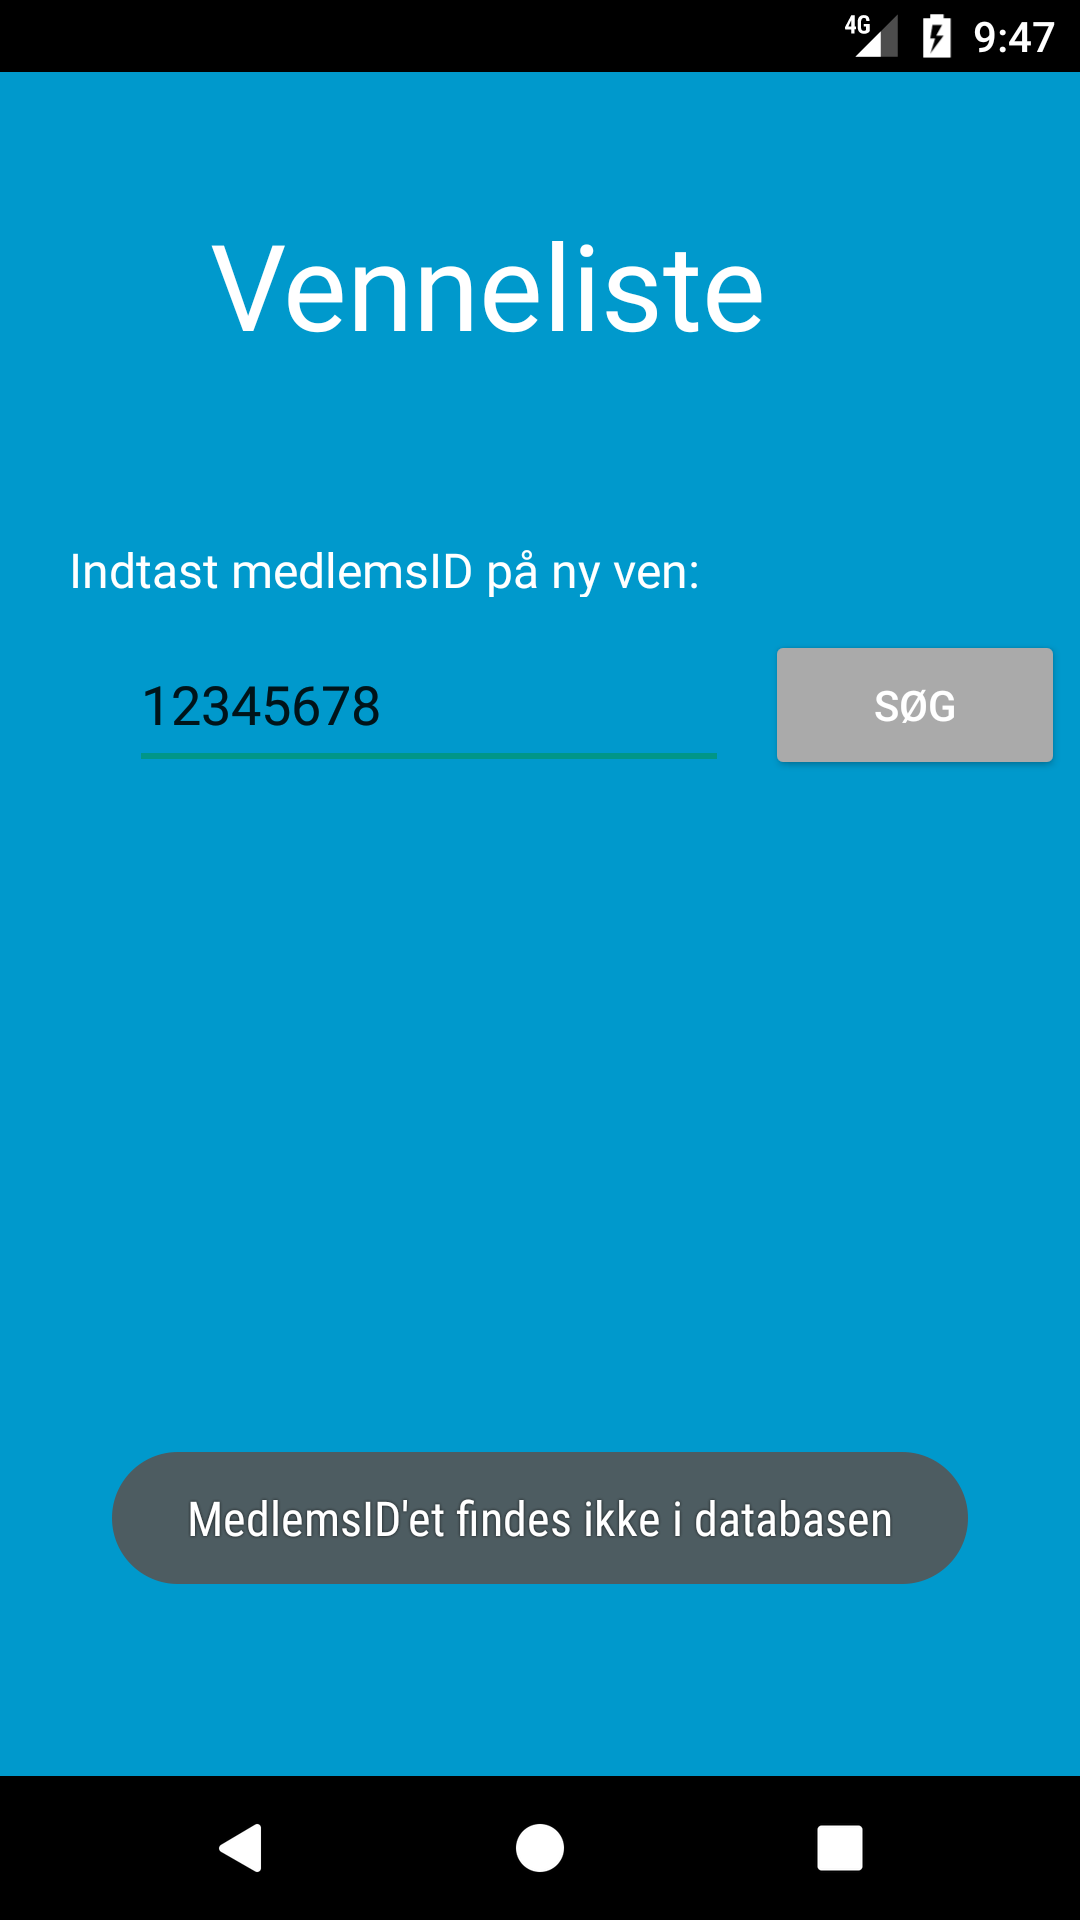
\includegraphics[width=0.20\textwidth, height=60mm]{figures/test/vennelisteny}} 
        \raisebox{-\totalheight}{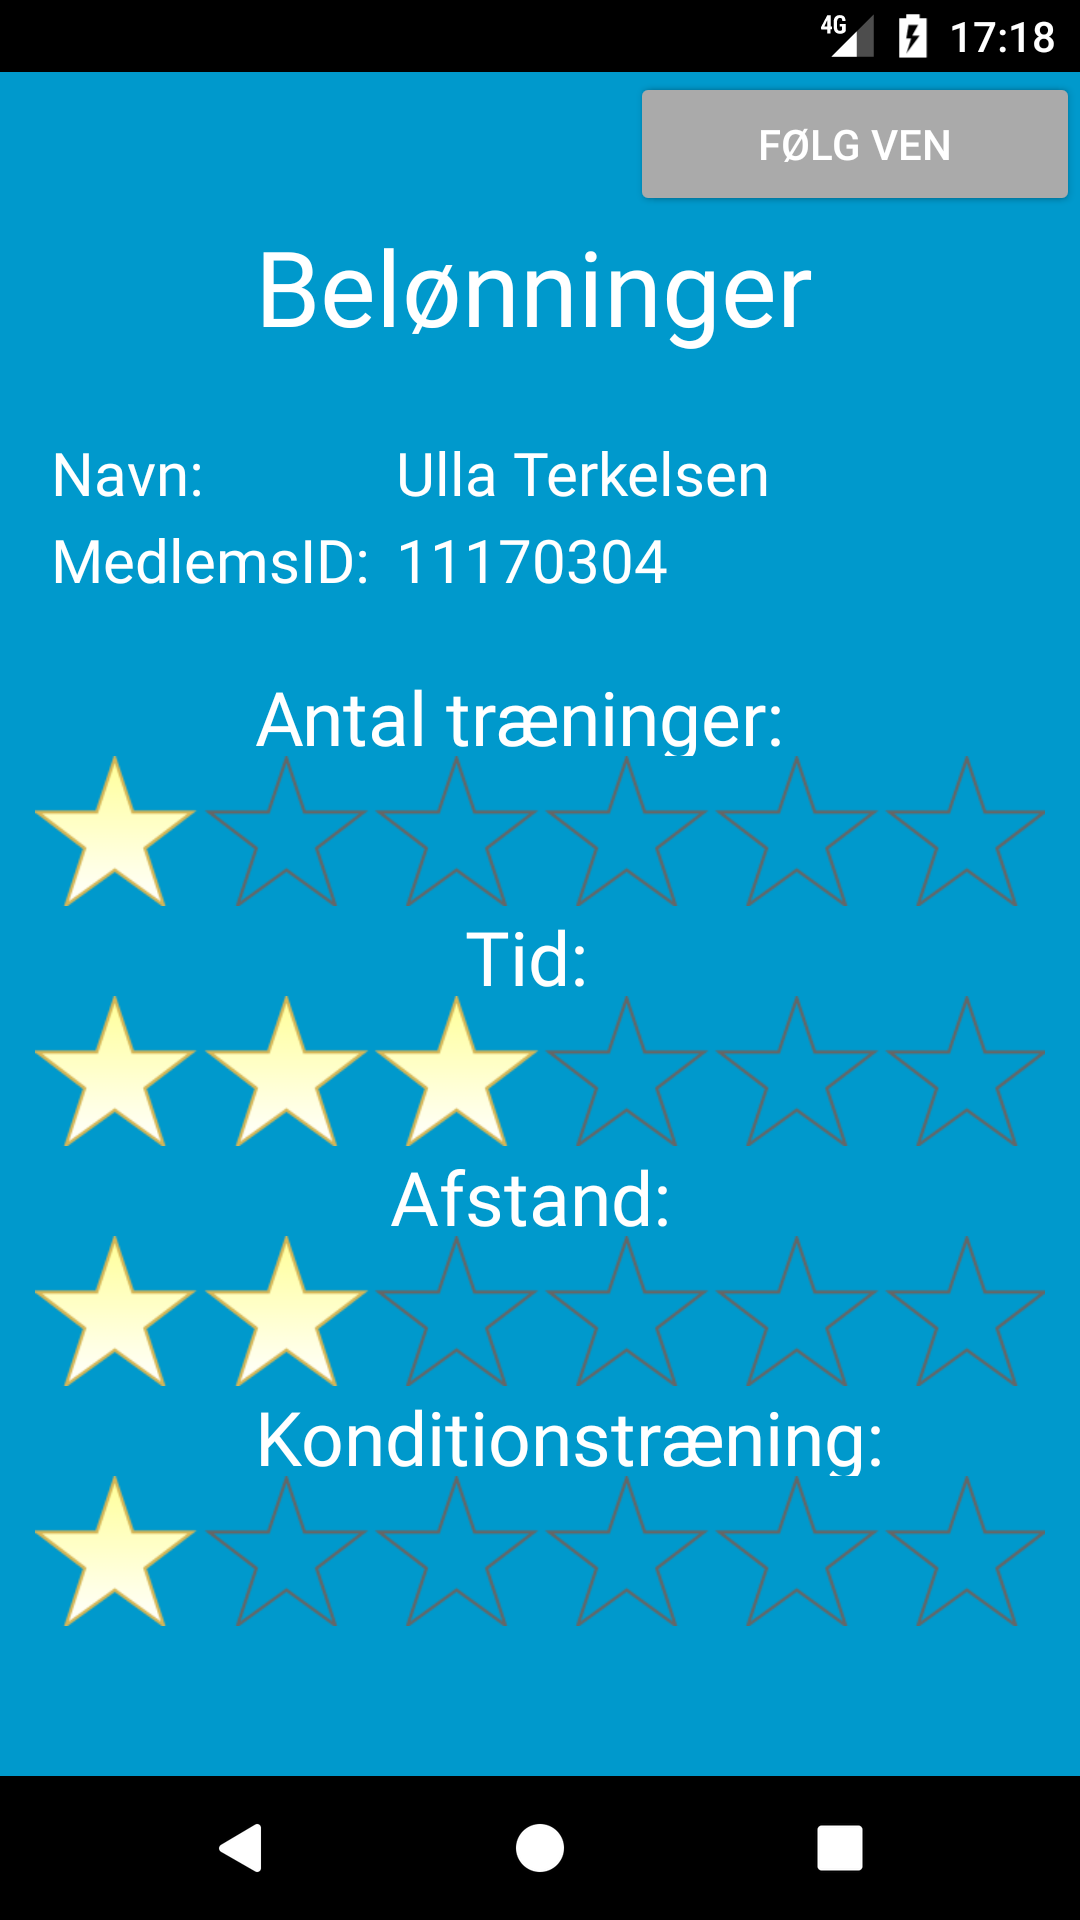
\includegraphics[width=0.20\textwidth, height=60mm]{figures/test/Vennelisteny1}} 
       \raisebox{-\totalheight}{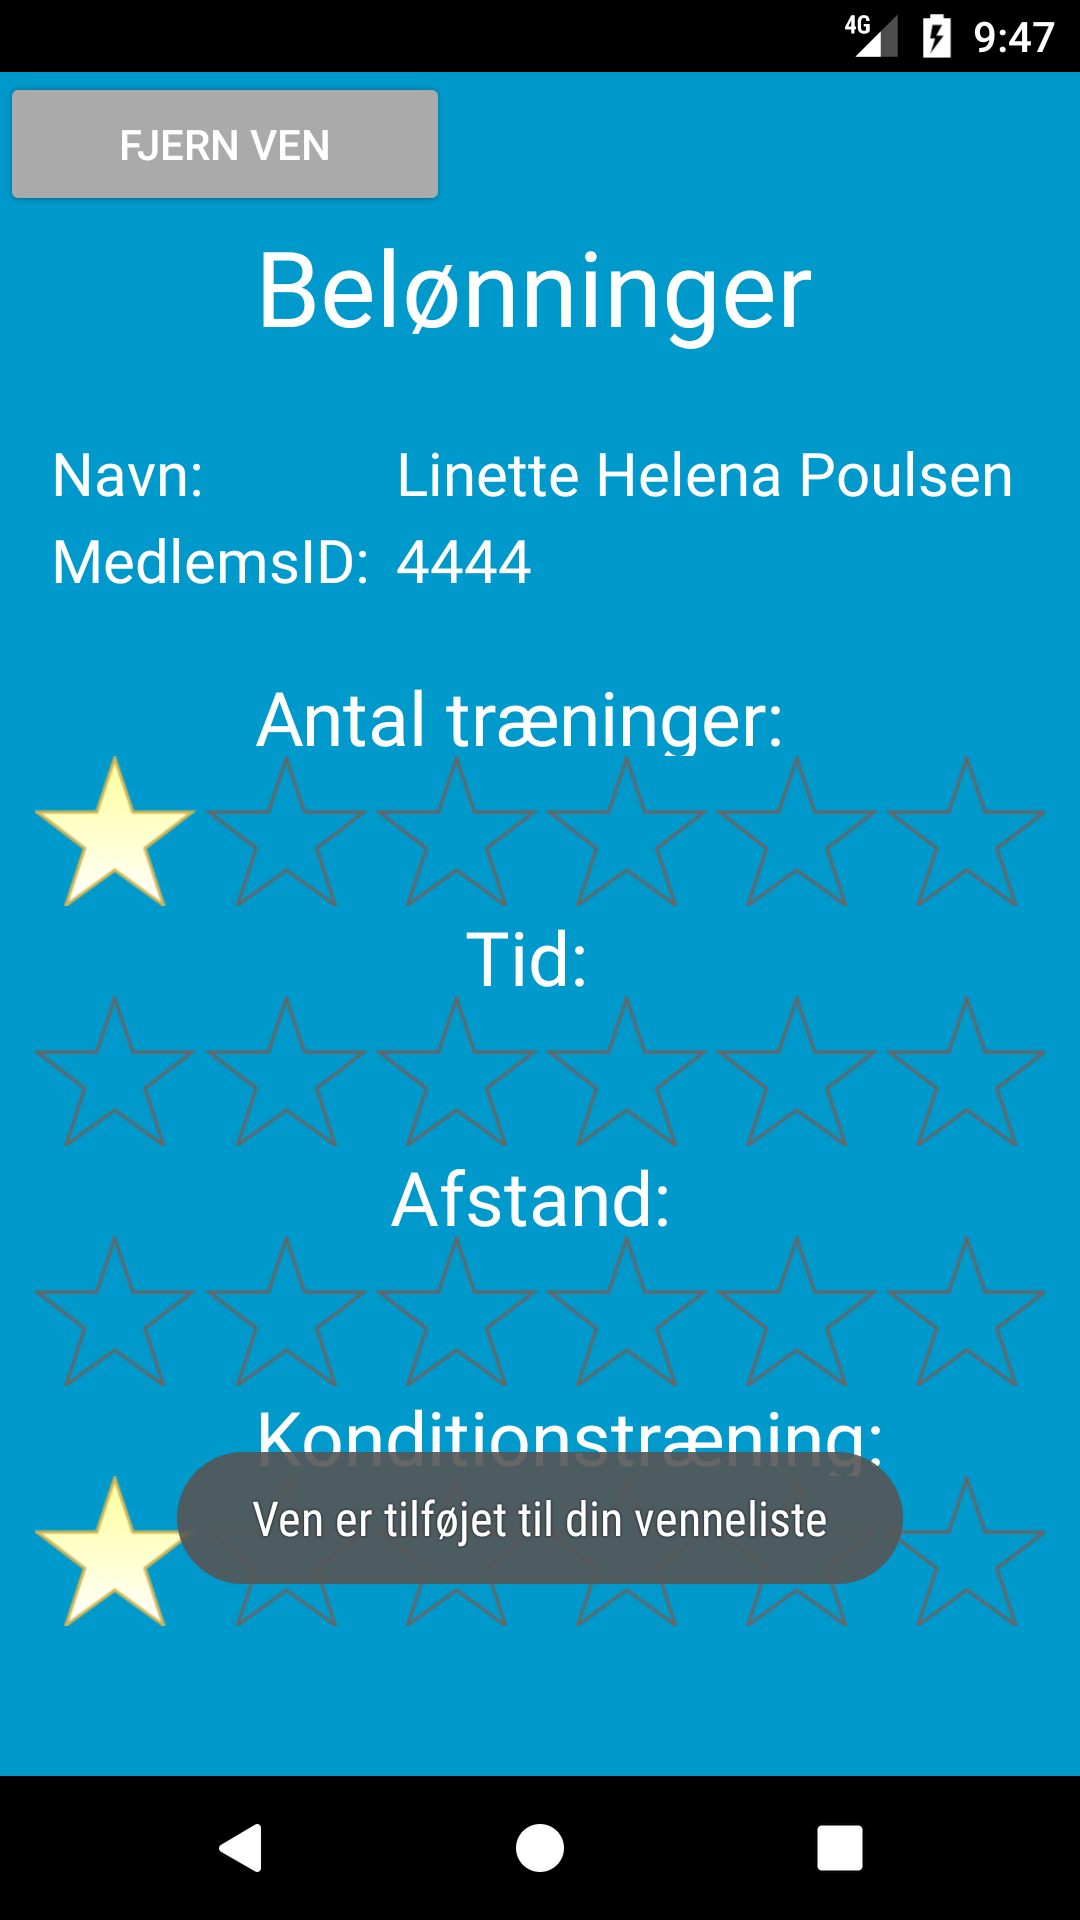
\includegraphics[width=0.20\textwidth, height=60mm]{figures/test/Vennelisteny2}} 
   \raisebox{-\totalheight}{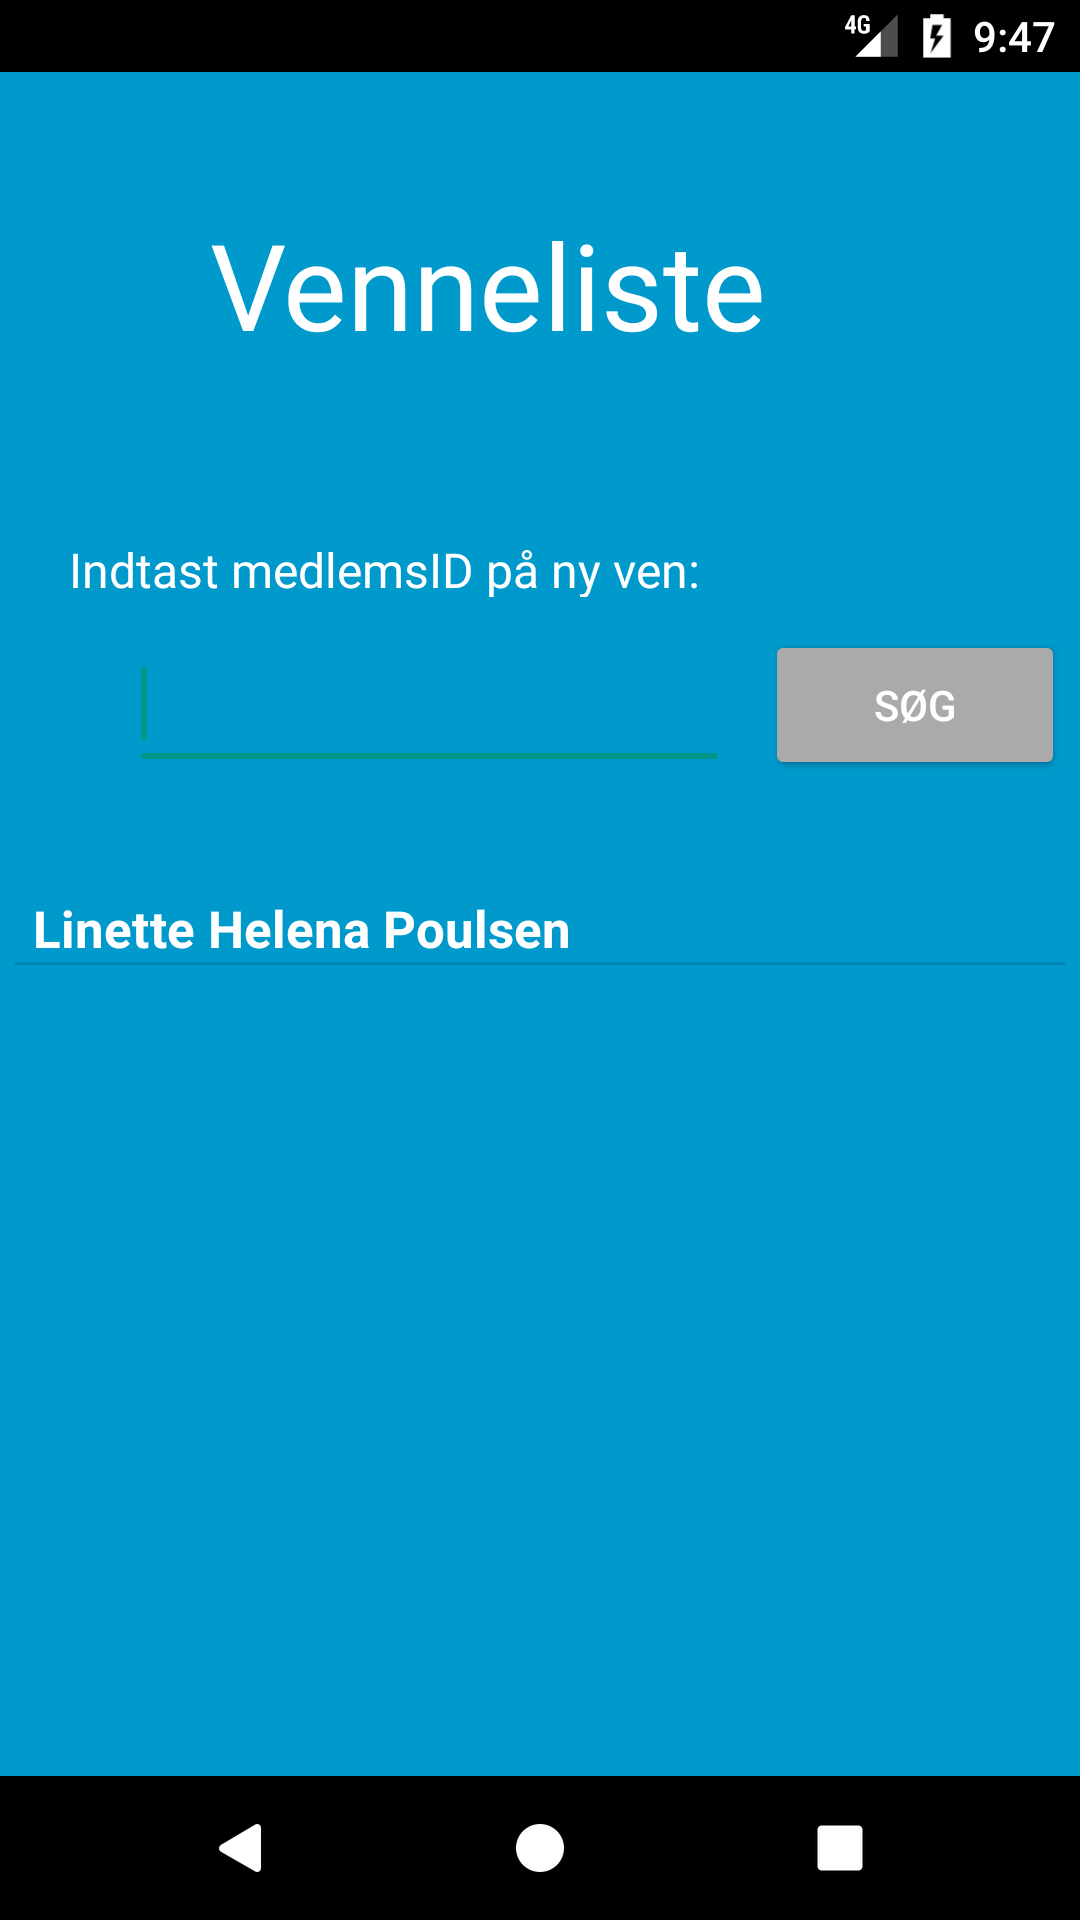
\includegraphics[width=0.20\textwidth, height=60mm]{figures/test/Vennelisteny3}}  
   \vspace{3mm}
             ~~~~~~~~\textbf{\textit{Figur 1}}~~~~~~~~~~~~~~\textbf{\textit{Figur 2}}~~~~~~~~~~~~~~~\textbf{\textit{Figur 3}}~~~~~~~~~~~~~~\textbf{\textit{Figur 4}}
    \newline
   Ovenstående figurer viser resultater for test af venneliste. Til venstre ses figur for første main flow, hvor det indtastede medlemsID ikke eksisterer i databasen. Figuren ved siden af viser andet main flow, hvor medlemsID'et eksisterer i databasen, og belønninger for denne bruger fremgår. Brugeren har mulighed for at tilføje ven til vennelisten, hvilket fremgår af de to figurer til højre, som opfylder tredje og fjerde main flow.
  \begin{itemize}[label={\checkmark}]
\item På baggrund af dette er kravet for venneliste opfyldt
\end{itemize}
    \\ \hline
   \caption{Test af venneliste.}
    \label{tab:testVenneliste}
\end{longtable}


\section{Redigering af adgangskode}
Redigering skal give brugeren mulighed for at redigere adgangskoden til en personlig adgangskode, da brugeren får udleveret en randomiseret adgangskode ved registreringen. Der er opstillet følgende krav for redigering:

\begin{itemize}
\item Brugere skal kunne redigere deres adgangskode
\\
\textit{Dette er nødvendigt for, at brugere skal kunne gøre deres adgangskode personlig}
\end{itemize}

\noindent
For at teste, hvorvidt kravene til redigering er overholdt, udføres testen, som fremgår af \autoref{tab:testRedigering}.

  \begin{longtable}{ | l | p{13cm} |} \hline
    \textbf{Test:} & Redigering \\ \hline
  \textbf{Formål:} & Formålet er, at brugeren skal have mulighed for at redigere sin adgangskode. Dette gøres ved at indtaste to forskellige adgangskoder og to ens adgangskoder. Efterfølgende logges der ind med den ændrede adgangskode.
 \\ \hline
 	\textbf{Main flow:} & 1.~Tryk \textit{REDIGER ADGANGSKODE} via hovedmenuen. Indtast \textit{nyadgangskode} i ny adgangskode og indtast \textit{adgangskode} i gentag adgangskode. Tryk \textit{GEM ÆNDRINGER}.   
 	\begin{itemize}
 	\item Ændring mislykkedes. Fejlmeddelelse vises i grænsefladen for redigering (\textbf{\textit{Figur 1}})
 	\end{itemize}	
 	2.~Tryk \textit{REDIGER ADGANGSKODE} via hovedmenuen. Indtast \textit{nyadgangskode} i ny adgangskode og gentag adgangskode. Tryk \textit{GEM ÆNDRINGER}. 
 	\begin{itemize}
 	\item Ændring lykkedes. Meddelelse viser, at adgangskoden er gemt (\textbf{\textit{Figur 2}})
 	\end{itemize}
 	3.~Log ud og log ind med medlemsID \textit{11170301} og den nye adgangskode \textit{nyadgangskode}.
 	\begin{itemize}
 	\item Log ind lykkes og hovedmenu vises  (\textbf{\textit{Figur 3 og 4}})
	\end{itemize} \\ \hline
\textbf{Resultat} &
    \raisebox{-\totalheight}    {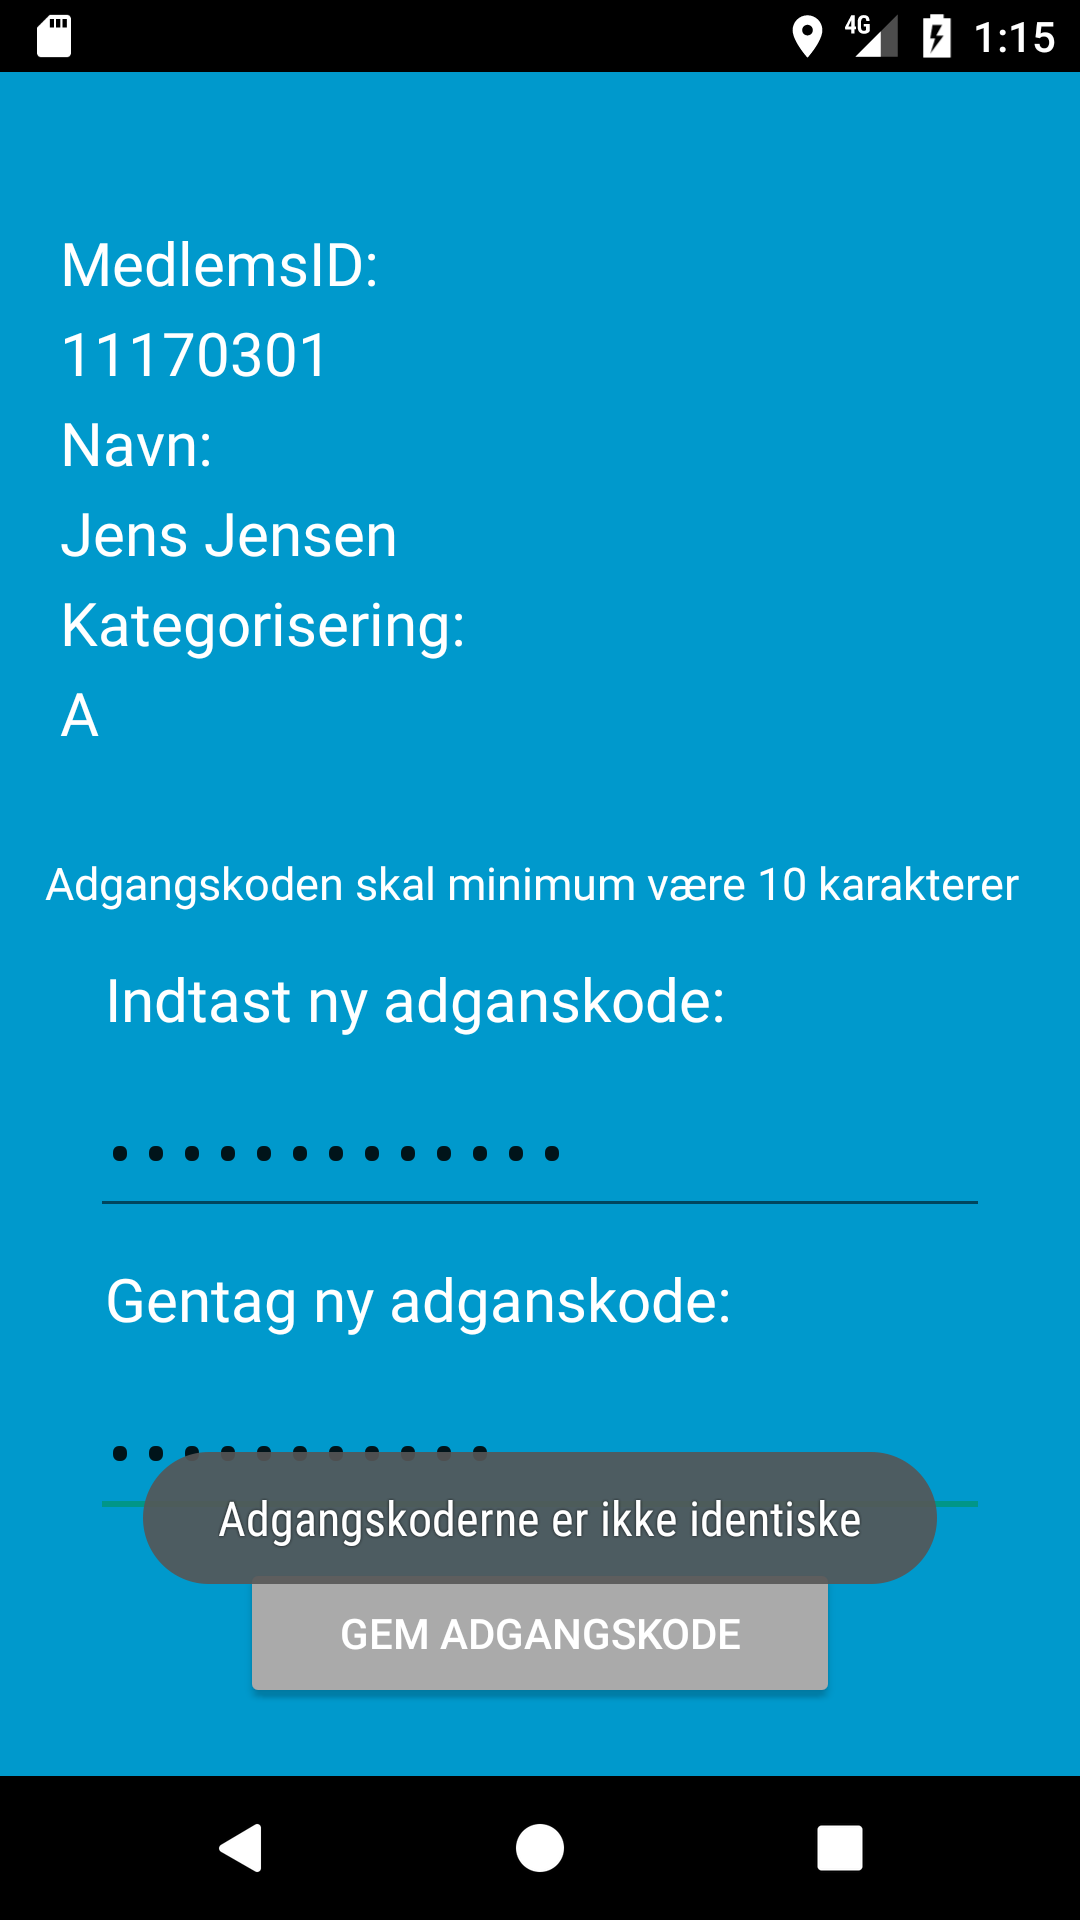
\includegraphics[width=0.20\textwidth, height=60mm]{figures/test/redigering2}} 
        \raisebox{-\totalheight}{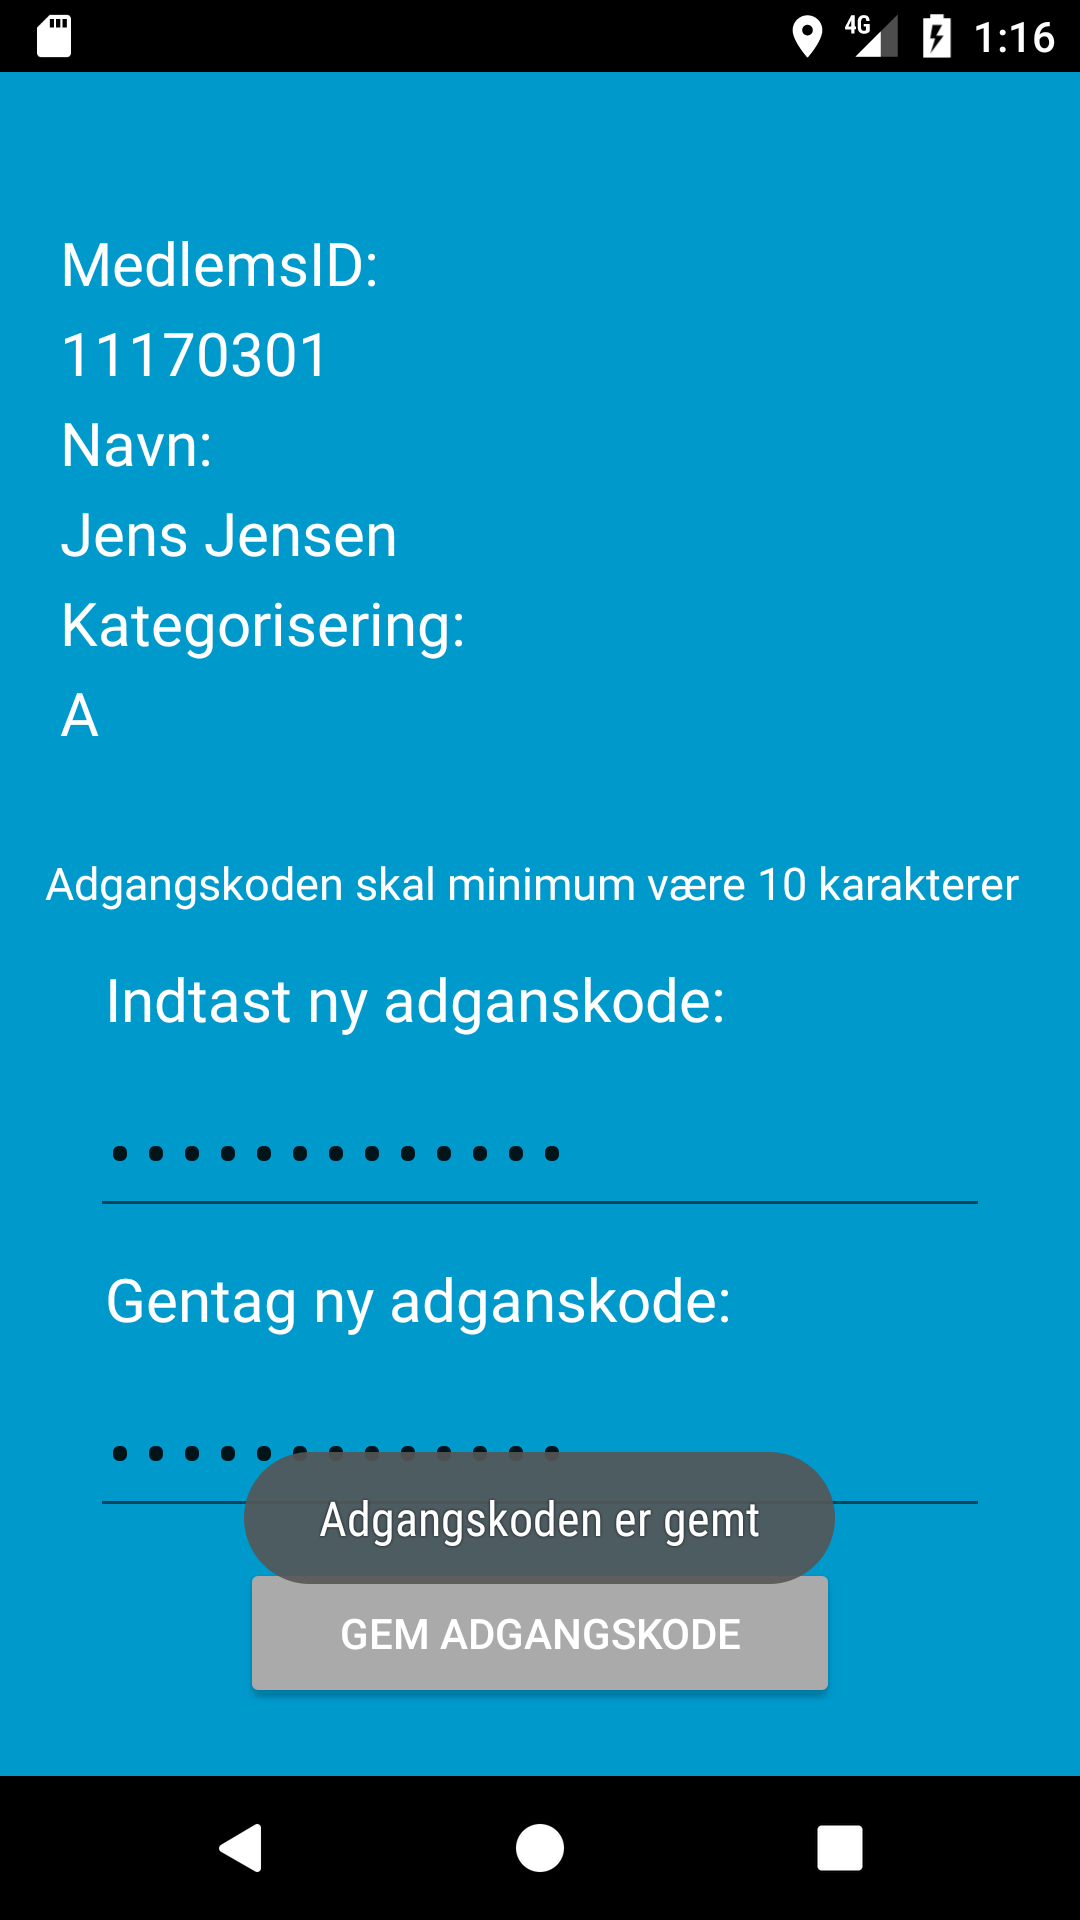
\includegraphics[width=0.20\textwidth, height=60mm]{figures/test/redigering3}} 
       \raisebox{-\totalheight}{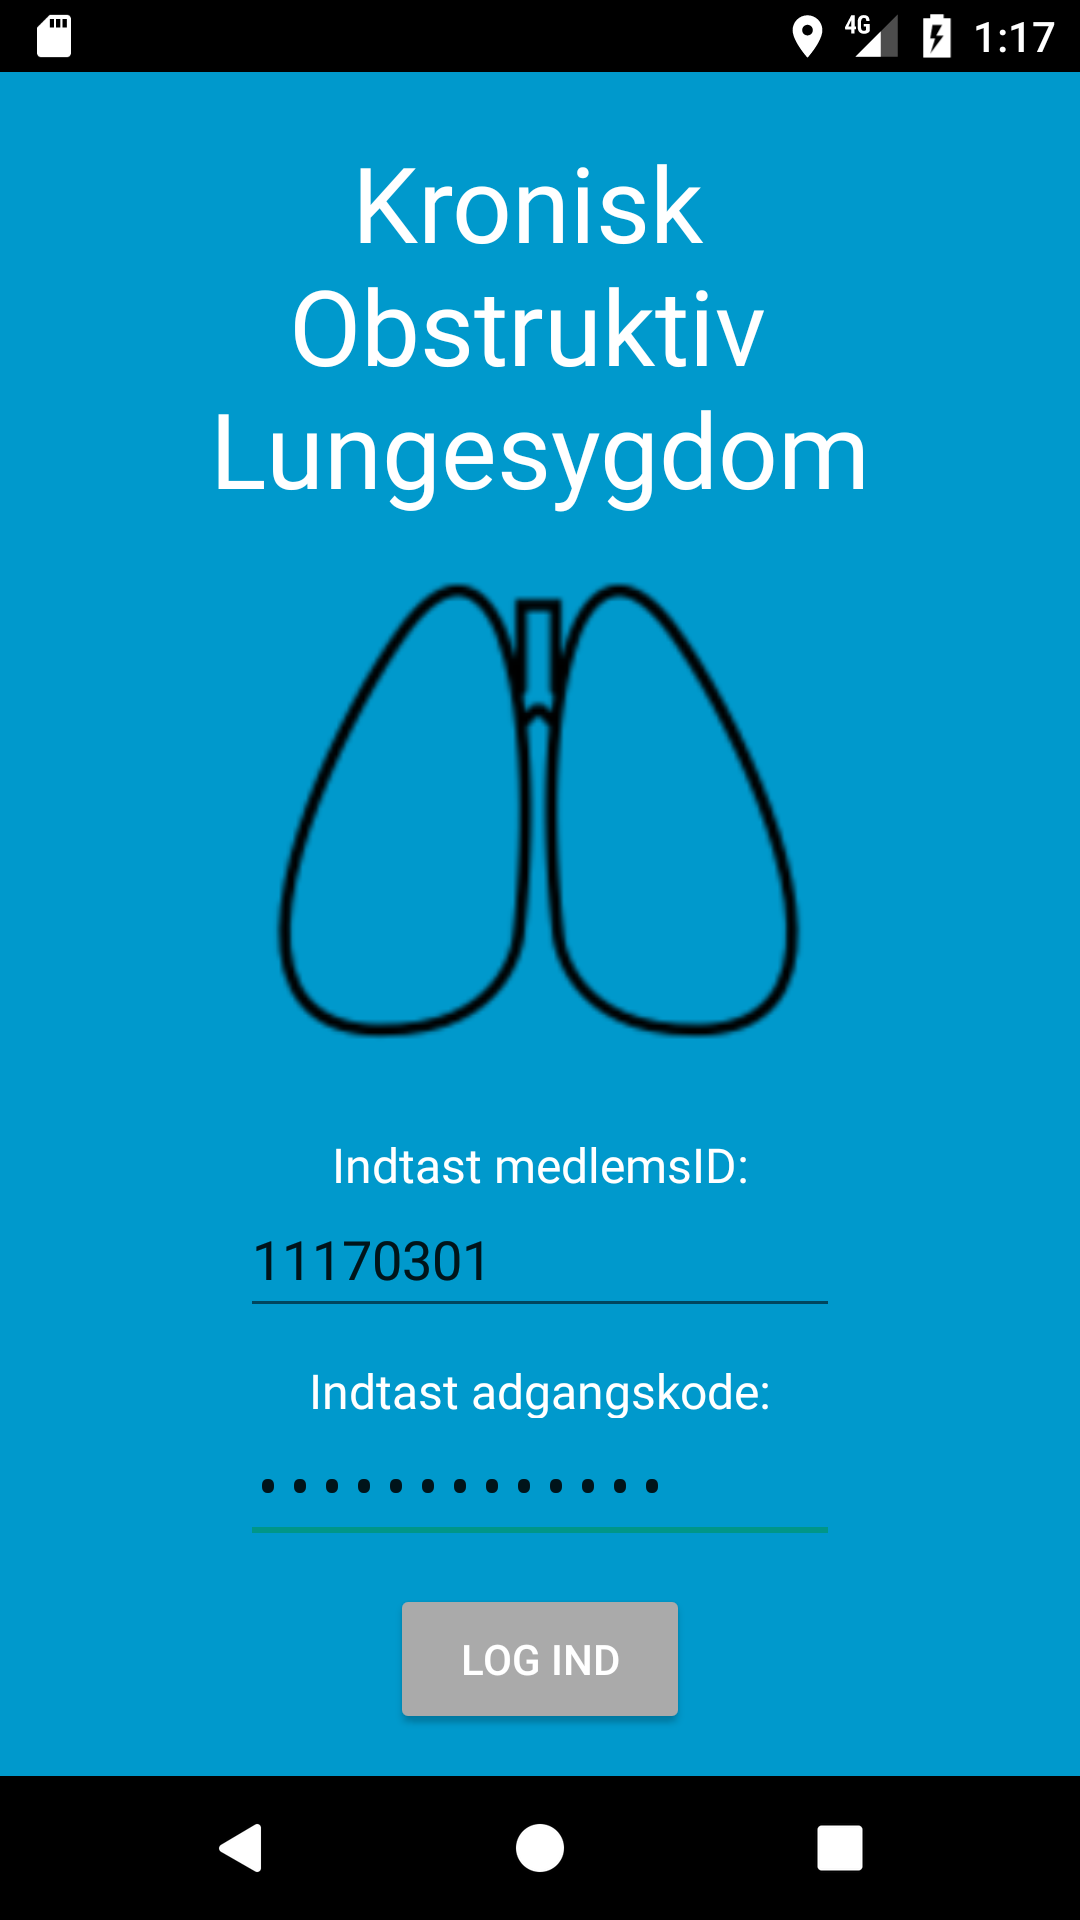
\includegraphics[width=0.20\textwidth, height=60mm]{figures/test/redigering}} 
   \raisebox{-\totalheight}{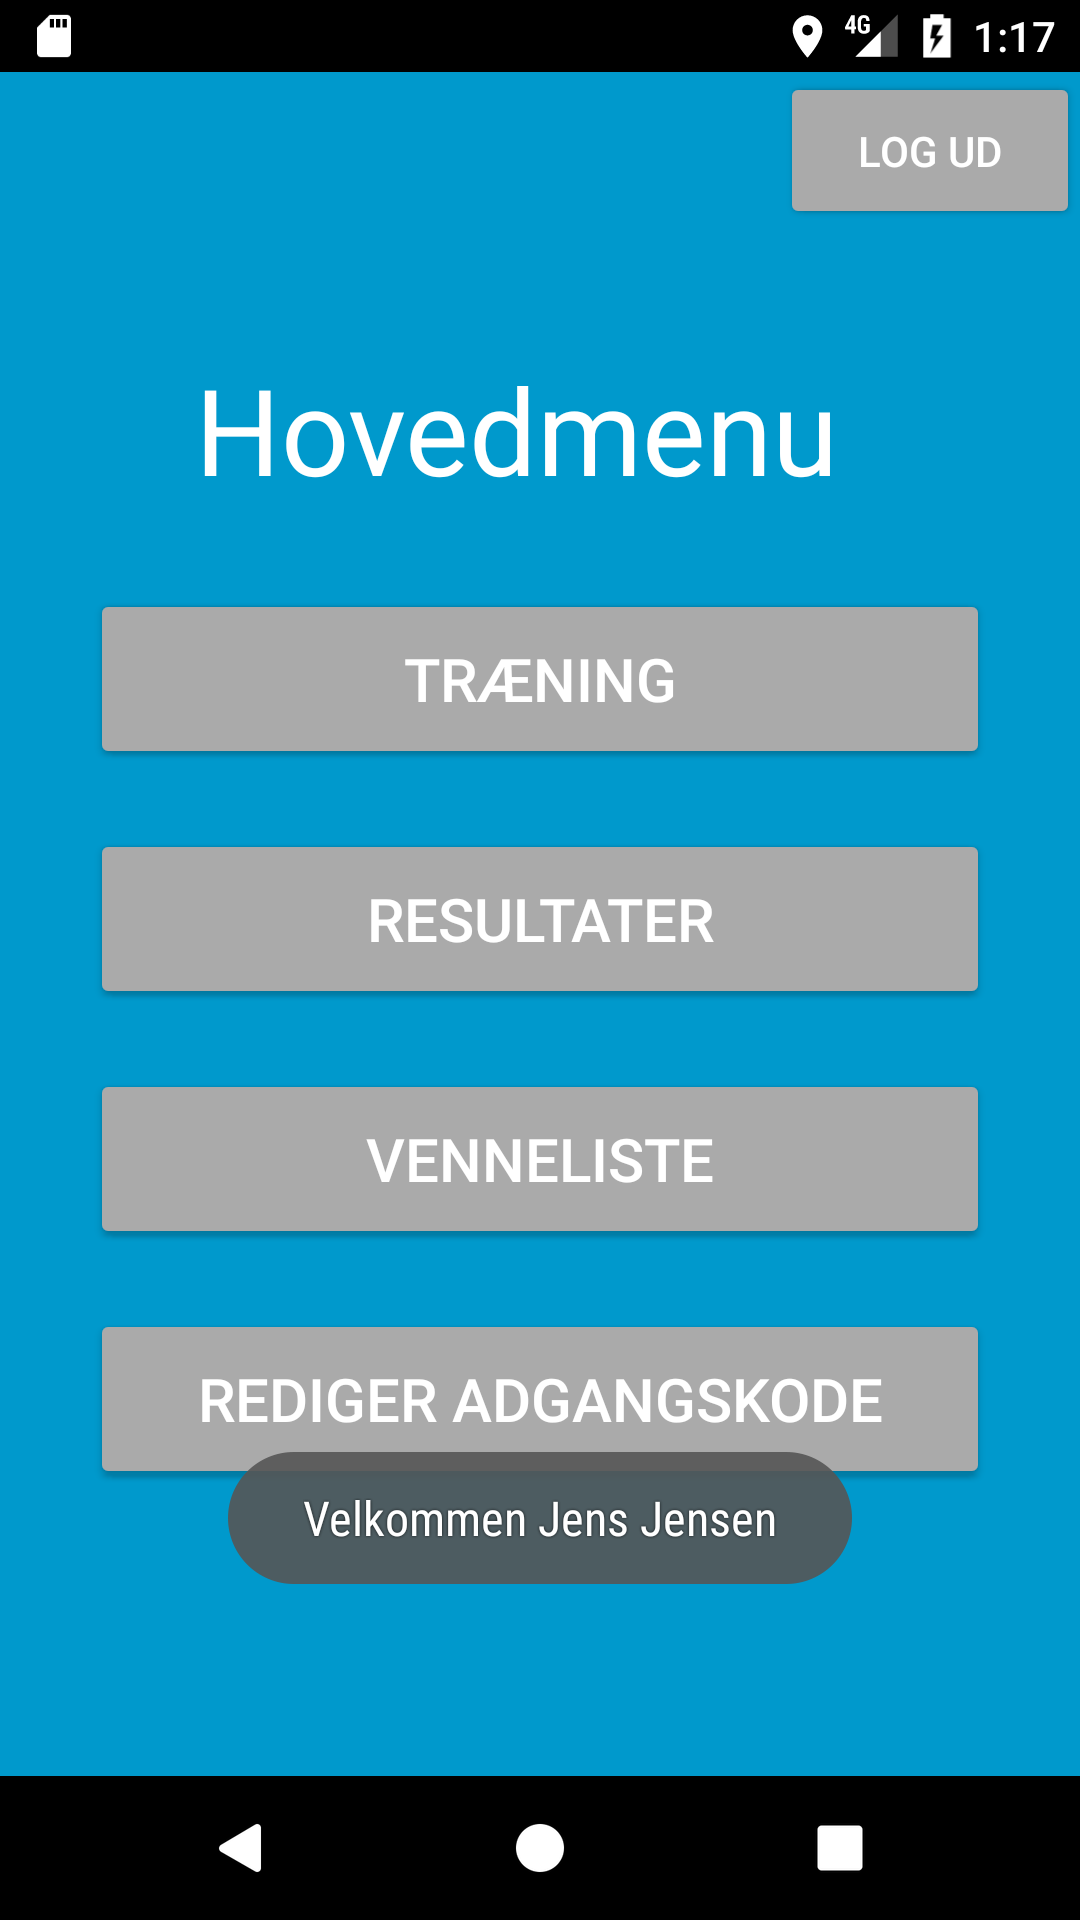
\includegraphics[width=0.20\textwidth, height=60mm]{figures/test/redigering1}}  \vspace{3mm}
               ~~~~~~~~\textbf{\textit{Figur 1}}~~~~~~~~~~~~~~\textbf{\textit{Figur 2}}~~~~~~~~~~~~~~~\textbf{\textit{Figur 3}}~~~~~~~~~~~~~~\textbf{\textit{Figur 4}}
    \newline
Ovenstående figurer viser resultater for test af redigering. Til venstre ses resultat for det første main flow, hvor det fremgår, at de indtastede adgangskoder ikke er identiske. Til venstre for midten er adgangskoderne identiske, hvorved disse gemmes i databasen. Test for det tredje main flow fremgår af de to figurer til højre, hvor der logges ind med den nye adgangskode og hovedmenuen vises.
 \begin{itemize}[label={\checkmark}]
\item På baggrund af dette er kravet for redigering 
\end{itemize}
    \\ \hline
   \caption{Test af redigering.}
    \label{tab:testRedigering}
\end{longtable}


\section{Log ud}
Log ud-funktionen skal sikre brugerens individuelle data. De opstillede krav til log ud er følgende:
\begin{itemize}
\item Brugere skal kunne logge ud af app’en
\\
\textit{Dette er nødvendigt for at sikre brugeres individuelle data og give brugeren mulighed for at logge ud}
\end{itemize}

\noindent
For at teste om ovenstående krav er opfyldt udføres testen, der fremgår af \autoref{tab:testLogud}.

  \begin{longtable}{ | l | p{13cm} |} \hline
    \textbf{Test:} & Log ud \\ \hline
  \textbf{Formål:} & Formålet er, at brugeren skal have mulighed for at logge ud af app’en.
 \\ \hline
 	\textbf{Main flow:} & 1.~Tryk \textit{LOG UD} via hovedmenuen og tryk bekræft.
 	\begin{itemize}
 	\item Grænseflade for log ind vises  (\textbf{\textit{Figur 3}})
 	\end{itemize}	
\\ \hline
\textbf{Resultat} &  \hspace{1.5mm}  \raisebox{-\totalheight}    {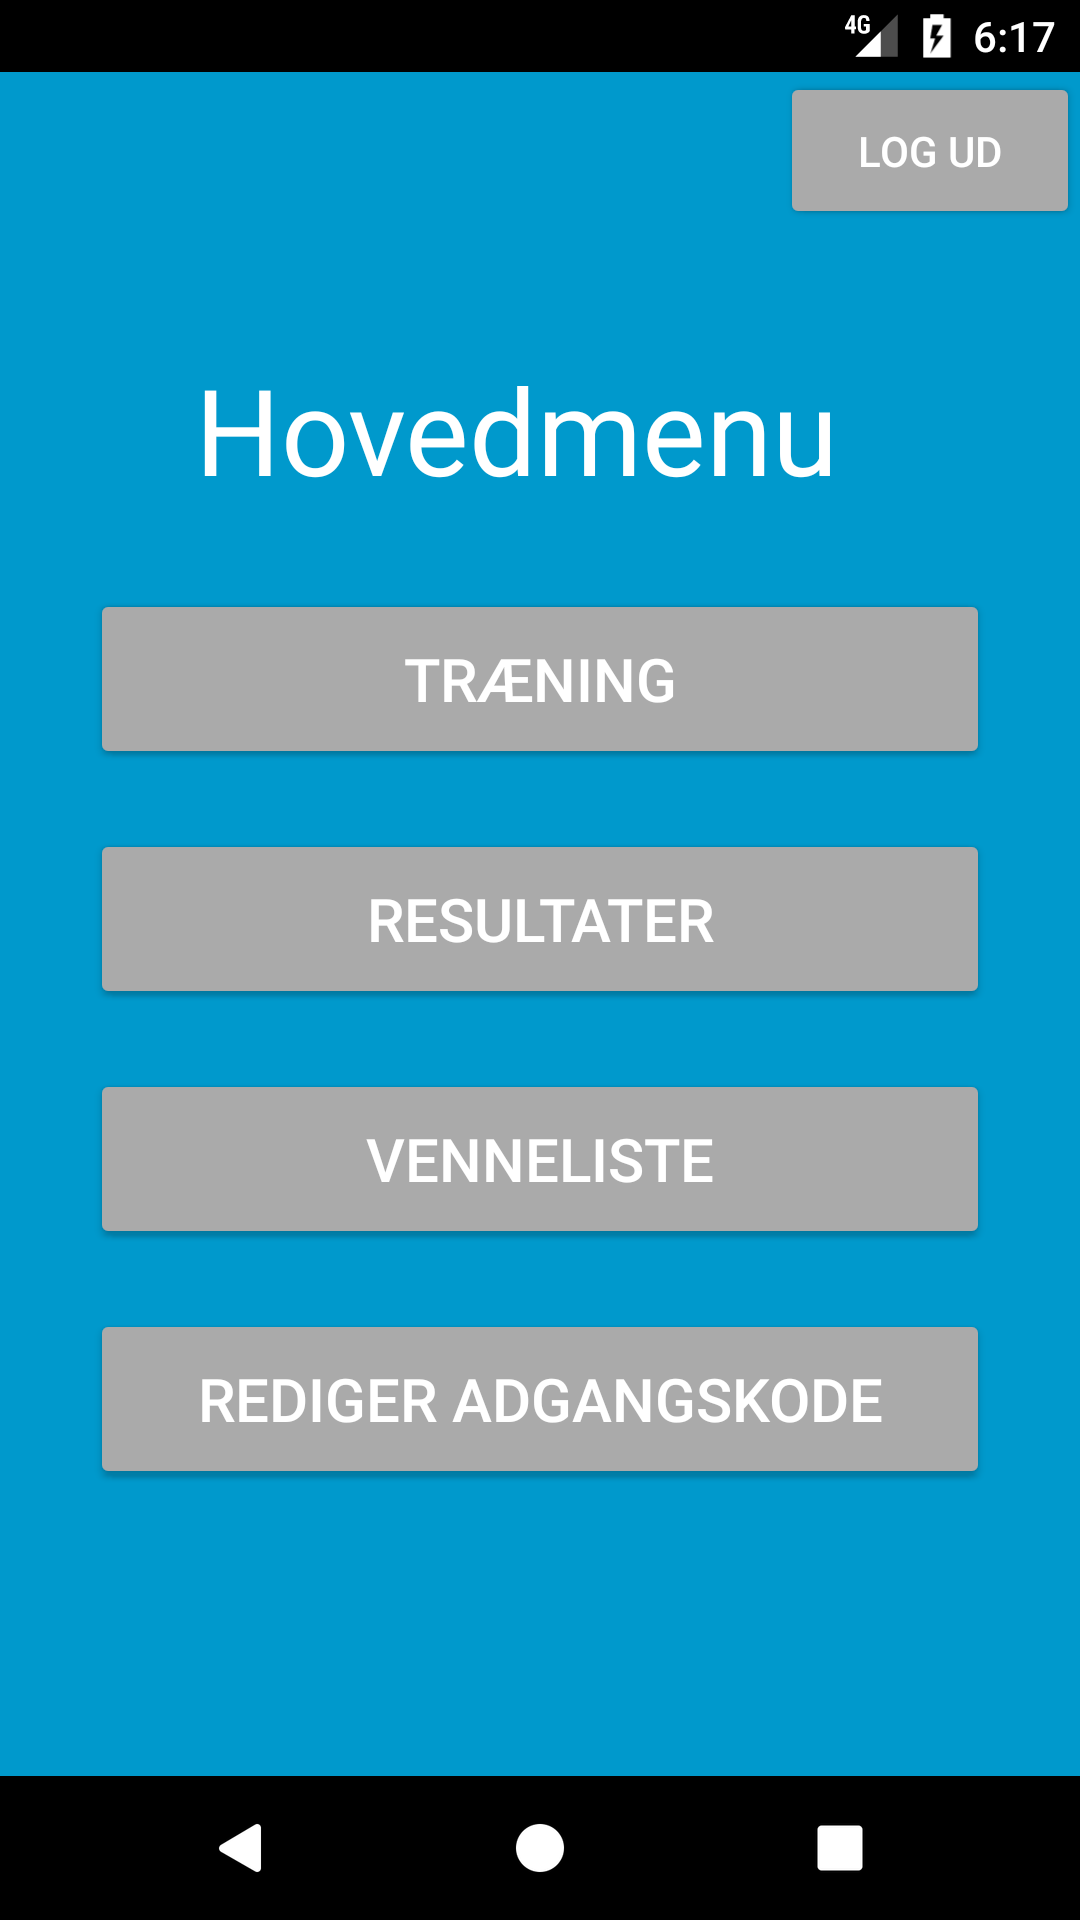
\includegraphics[width=0.24\textwidth, height=60mm]{figures/test/logud2}} 
\hspace{5mm}
        \raisebox{-\totalheight}
    {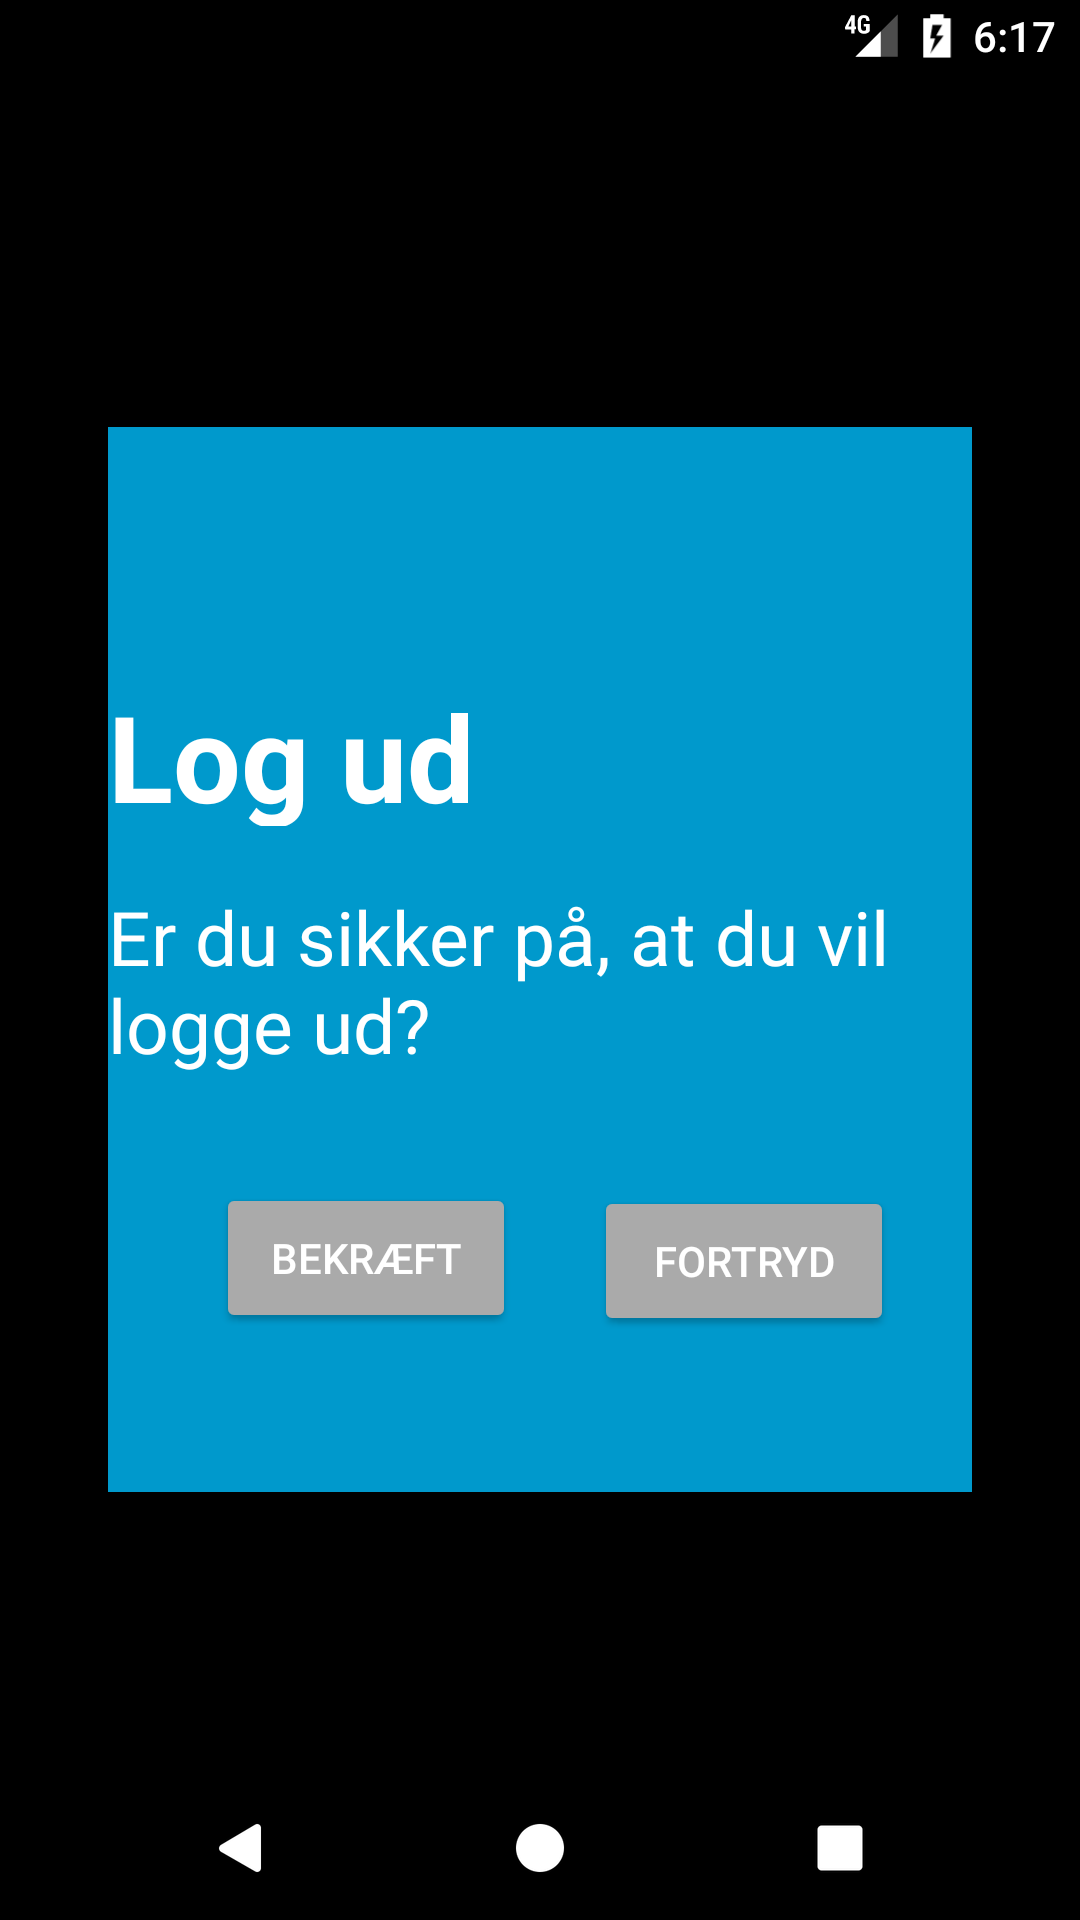
\includegraphics[width=0.24\textwidth, height=60mm]{figures/test/logud3}} 
    \hspace{5mm}
        \raisebox{-\totalheight}
    {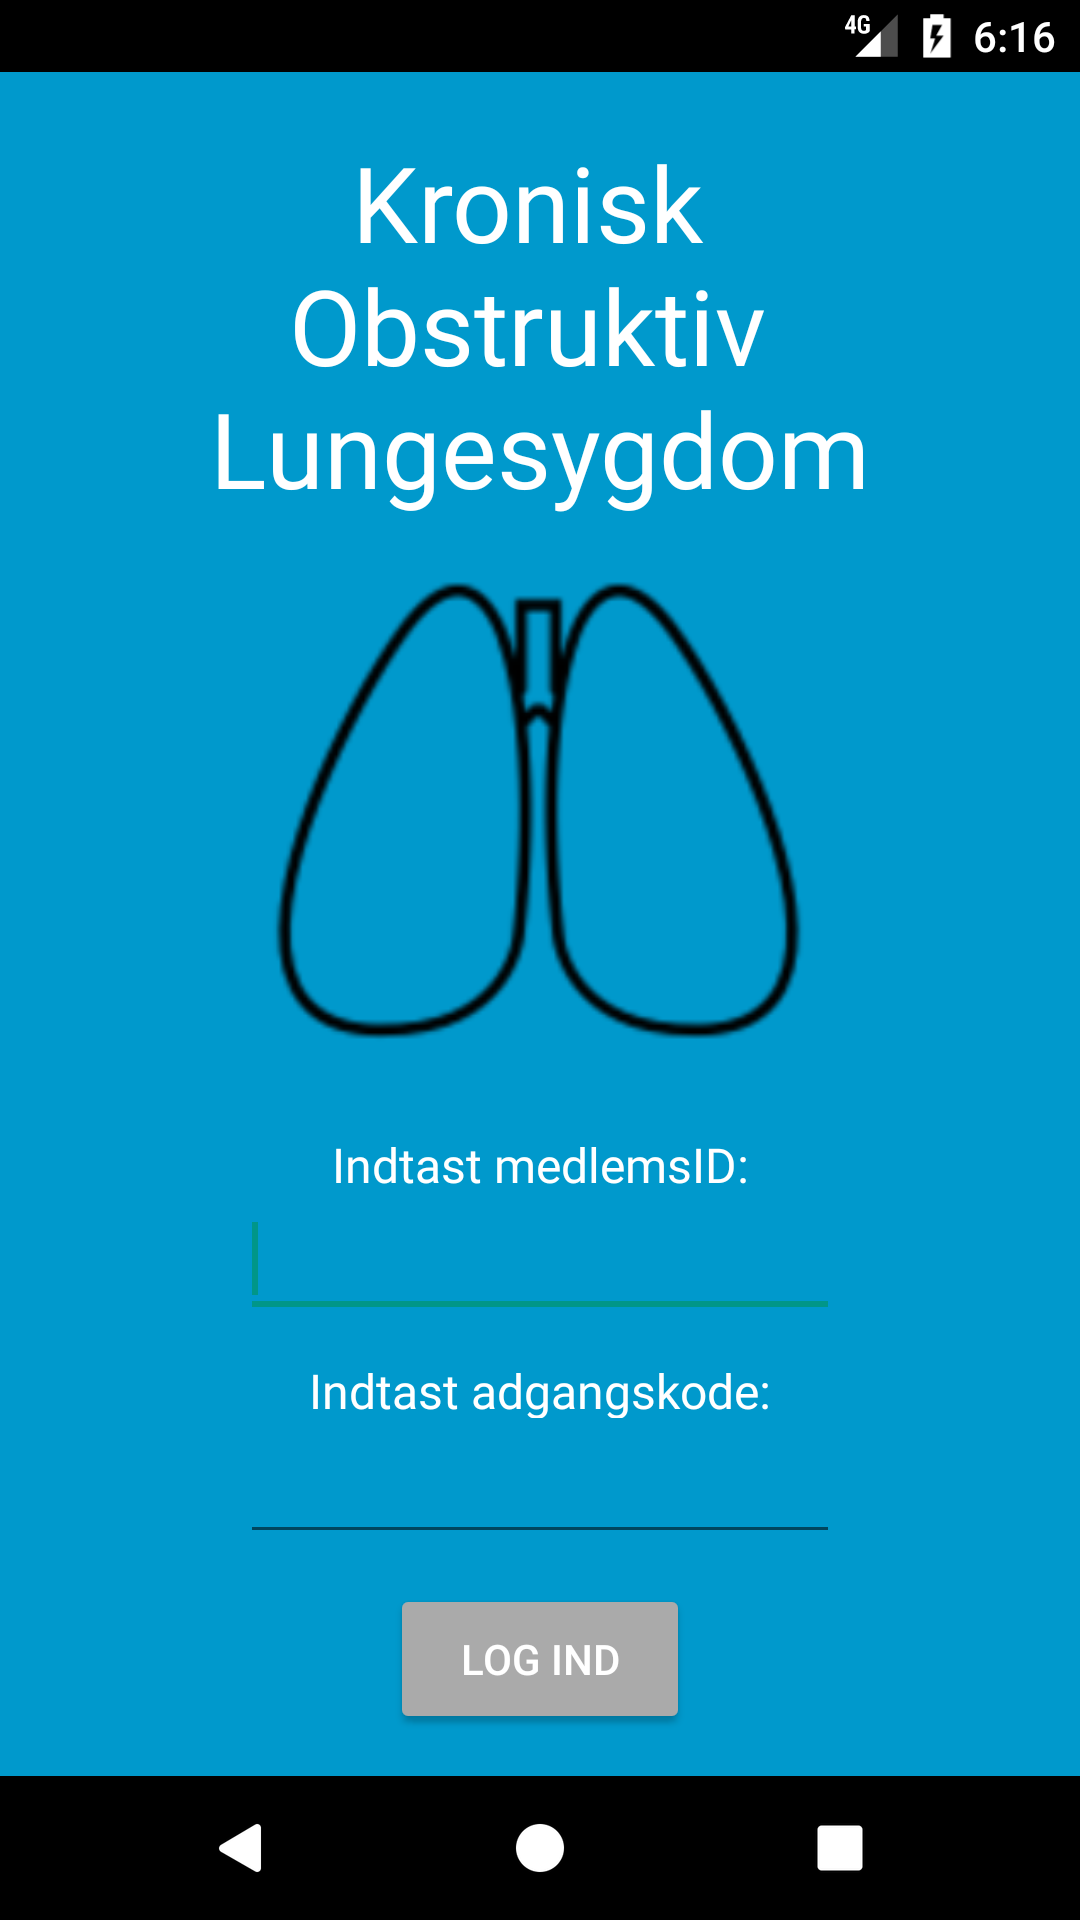
\includegraphics[width=0.24\textwidth, height=60mm]{figures/test/logud1}} \vspace{3mm}
                ~~~~~~~~~~~ \textbf{\textit{Figur 1}}~~~~~~~~~~~~~~~~~~~~~~~~\textbf{\textit{Figur 2}}~~~~~~~~~~~~~~~~~~~~~~~~\textbf{\textit{Figur 3}}
       \newline
Figurerne ovenfor viser resultater for test af log ud. Til venstre ses hovedmenuen, hvor brugeren har mulighed for at logge ud. I midten skal brugeren bekræfte log ud, hvis dette gøres vises grænsefladen for log ind, som ses af figuren til højre.
 \begin{itemize}[label={\checkmark}]
\item Ud fra denne test er kravet for log ud opfyldt
\end{itemize}
    \\ \hline
   \caption{Test af log ud.}
    \label{tab:testLogud}
\end{longtable}





